\usepackage{wx672tut}

\newcommand{\unix}{{\fontspec{Purisa}{UNIX}}}
\newcommand{\emacs}{
\includegraphics[width=1.2em]{emacs}}
\newcommand{\google}{\raisebox{-.2em}{\includegraphics[width=3em]{google}}}
\newcommand{\GG}{\textcolor{SkyBlue}{\nerd }}
\newcommand{\world}{\textcolor{SkyBlue}{\nerd }}
\newcommand{\pdf}{\textcolor{red}{\nerd }}%
\newcommand{\folder}{{\nerd }}%e5fe,e61e,e7a3,f07c
\newcommand{\git}{{\nerd }}%f1d2,f1d3
\newcommand{\github}{\nerd }
\newcommand{\moodle}{
\includegraphics[width=1em]{moodle}}
\newcommand{\obook}{{\nerd }}%f212,f401,f405
\newcommand{\shell}{{\nerd }}%e795
\newcommand{\CMD}[1]{\texttt{\textcolor{Green}{\$} #1}}
\newcommand{\cmd}[1]{\texttt{#1}}
\newcommand{\vim}{{\nerd }}
\newcommand{\stackoverflow}{{\nerd }}%f16c, e710
\newcommand{\correct}{{\Large\textcolor{Green}{\nerd ✔}}}
\newcommand{\wrong}{\textcolor{red}{\nerd ✘}}
\newcommand{\Bad}{{\Large \textcolor{red}{\bad}}}
\newcommand{\Good}{{\Large \textcolor{Green}{\good}}}
\newcommand{\phone}{\nerd fi} % 260e☎ fb01fi
\newcommand{\mail}{\nerd } %f42f f6ef f6ed faee﫮 faef﫯 f430 
\newcommand{\hw}{\nerd } %f8ec f8ea f420 f26d f14b f0e7 e30e e315 e305

% f421,f46e,f536 f1e6 

\addbibresource{ref.bib}

\newcommand{\textbooks}{\nocite{cs241, matthew2008beginning, cooper10bash, raymond2003art,
    stevens2013advanced, Love:2007:LSP:1205435, Kerrisk:2010:LPI:1869911,
    Bryant2010computersystems}}%

%\AtBeginPart{\frame{\partpage}}
\mode<beamer>{
  \AtBeginSection{\frame{\sectionpage}}
  \AtBeginSubsection{\frame{\subsectionpage}}
}

% \includeonlylecture{intro}
% \includeonlylecture{ipc}

\title{GNU/Linux\\Application Programming}
\author{WANG Xiaolin\\%
  {\footnotesize\texttt{wx672ster+linux@gmail.com}}}

\begin{document}

\mode<article>{  
  \subtitle{Lecture Handouts}
  \maketitle
  \tableofcontents
  \textbooks \printbibliography[title={References}]}

\mode<beamer>{\frame{\titlepage}}

\begin{frame}<beamer>{Reference Books}
  \begin{refsection}
    \textbooks \printbibliography[heading=none]
  \end{refsection}
\end{frame}

\begin{frame}{Course Web Links}
  \begin{itemize}
  \item[\moodle] \url{https://cs6.swfu.edu.cn/moodle}
  \item[\pdf] \url{https://cs2.swfu.edu.cn/~wx672/lecture_notes/linux-app/slides/}
  \item[\folder] \url{https://cs2.swfu.edu.cn/~wx672/lecture_notes/linux-app/src/}
  \item[\obook] \url{https://cs3.swfu.edu.cn/tech}
  \end{itemize}
  \begin{block}{\texttt{/etc/hosts}}
    \ttfamily
    \begin{tabular}{ll}
      202.203.132.241&cs6.swfu.edu.cn\\      
      202.203.132.242&cs2.swfu.edu.cn\\
      202.203.132.245&cs3.swfu.edu.cn\\      
    \end{tabular}
  \end{block}\footnotesize
  \begin{description}
  \item[System Programming] \url{https://github.com/angrave/SystemProgramming/wiki}
  \item[Beej's Guides] \url{http://beej.us/guide/}
  \item[BLP4e] \url{http://www.wrox.com/WileyCDA/WroxTitle/productCd-0470147628,descCd-DOWNLOAD.html}
  \item[TLPI] \url{http://www.man7.org/tlpi/}
  \end{description}
\end{frame}

\begin{frame}{{\hw\enspace}Homework}
  \begin{block}{Weekly tech question}
    \begin{enumerate}
    \item What was I trying to do?
    \item How did I do it? (steps)
    \item The expected output? The real output?
    \item How did I try to solve it? (steps, books, web links)
    \item How many hours did I struggle?
    \end{enumerate}
  \end{block}
  \begin{itemize}
  \item[\Large\dejavu ✉] \alert{\ttfamily wx672ster+linux@gmail.com}
  \item[$\mathbb{E}$] Preferably in English
  \item[\stackoverflow] in
    \href{https://stackoverflow.com/questions/39199299/what-is-the-essential-difference-between-compound-command-and-normal-command-inlink}{stackoverflow}
    style
  \item[OR] simply show me the tech questions you asked on any website
  \end{itemize}  
\end{frame}

\begin{frame}
  \mode<beamer>{%
    \begin{tikzpicture}[remember picture, overlay]
      \node at (current page.center) [scale=20,opacity=.1] {\danger};%
      \node at (current page.center) [scale=2.8,rotate=30,align=center,font=\humor]%
      {Oversimplifed programs\\ahead!};
    \end{tikzpicture}}
  \begin{center}
    \mode<article>{
      \begin{itemize}
      \item[\danger] Oversimplifed programs ahead!
      \end{itemize}}
  \end{center}
\end{frame}

\lecture{start}{start}% \lecture[short name]{name}{label}
\section{Getting Started}
\label{sec:start}

\begin{frame}{Linux Commands}
  \begin{description}
  \item[Where to find them?] {\ttfamily /bin, /usr/bin, /usr/local/bin,\\\symbol{`~}/bin,
      \ldots}
    \begin{itemize}
    \item[\$] \texttt{echo \$PATH}
    \end{itemize}
  \item[How to find them?] \texttt{which, whereis, type}
  \end{description}
  \begin{block}{Command not found?}
    \begin{description}
    \item[First] double check your spelling
    \item[Then] try:{\ttfamily
      \begin{itemize}
      \item[\debian] aptitude search xxx
      \item[\debian] apt-cache search xxx
      \item[\debian] apt-file search xxx
      \item[\debian] sudo apt install packagename
      \item[\GG] \google~"linux command xxx"
      \end{itemize}}
    \end{description}
  \end{block}
\end{frame}

\begin{frame}{Text Editors}
  \begin{block}
    {\mode<beamer>{{{\Huge\vim}\,\quad{}vs.\quad{}{\LARGE\emacs}}}
    \mode<article>{{\vim\,\quad{}vs.\quad{}\emacs}}}
    \begin{center}
      \mode<beamer>{ 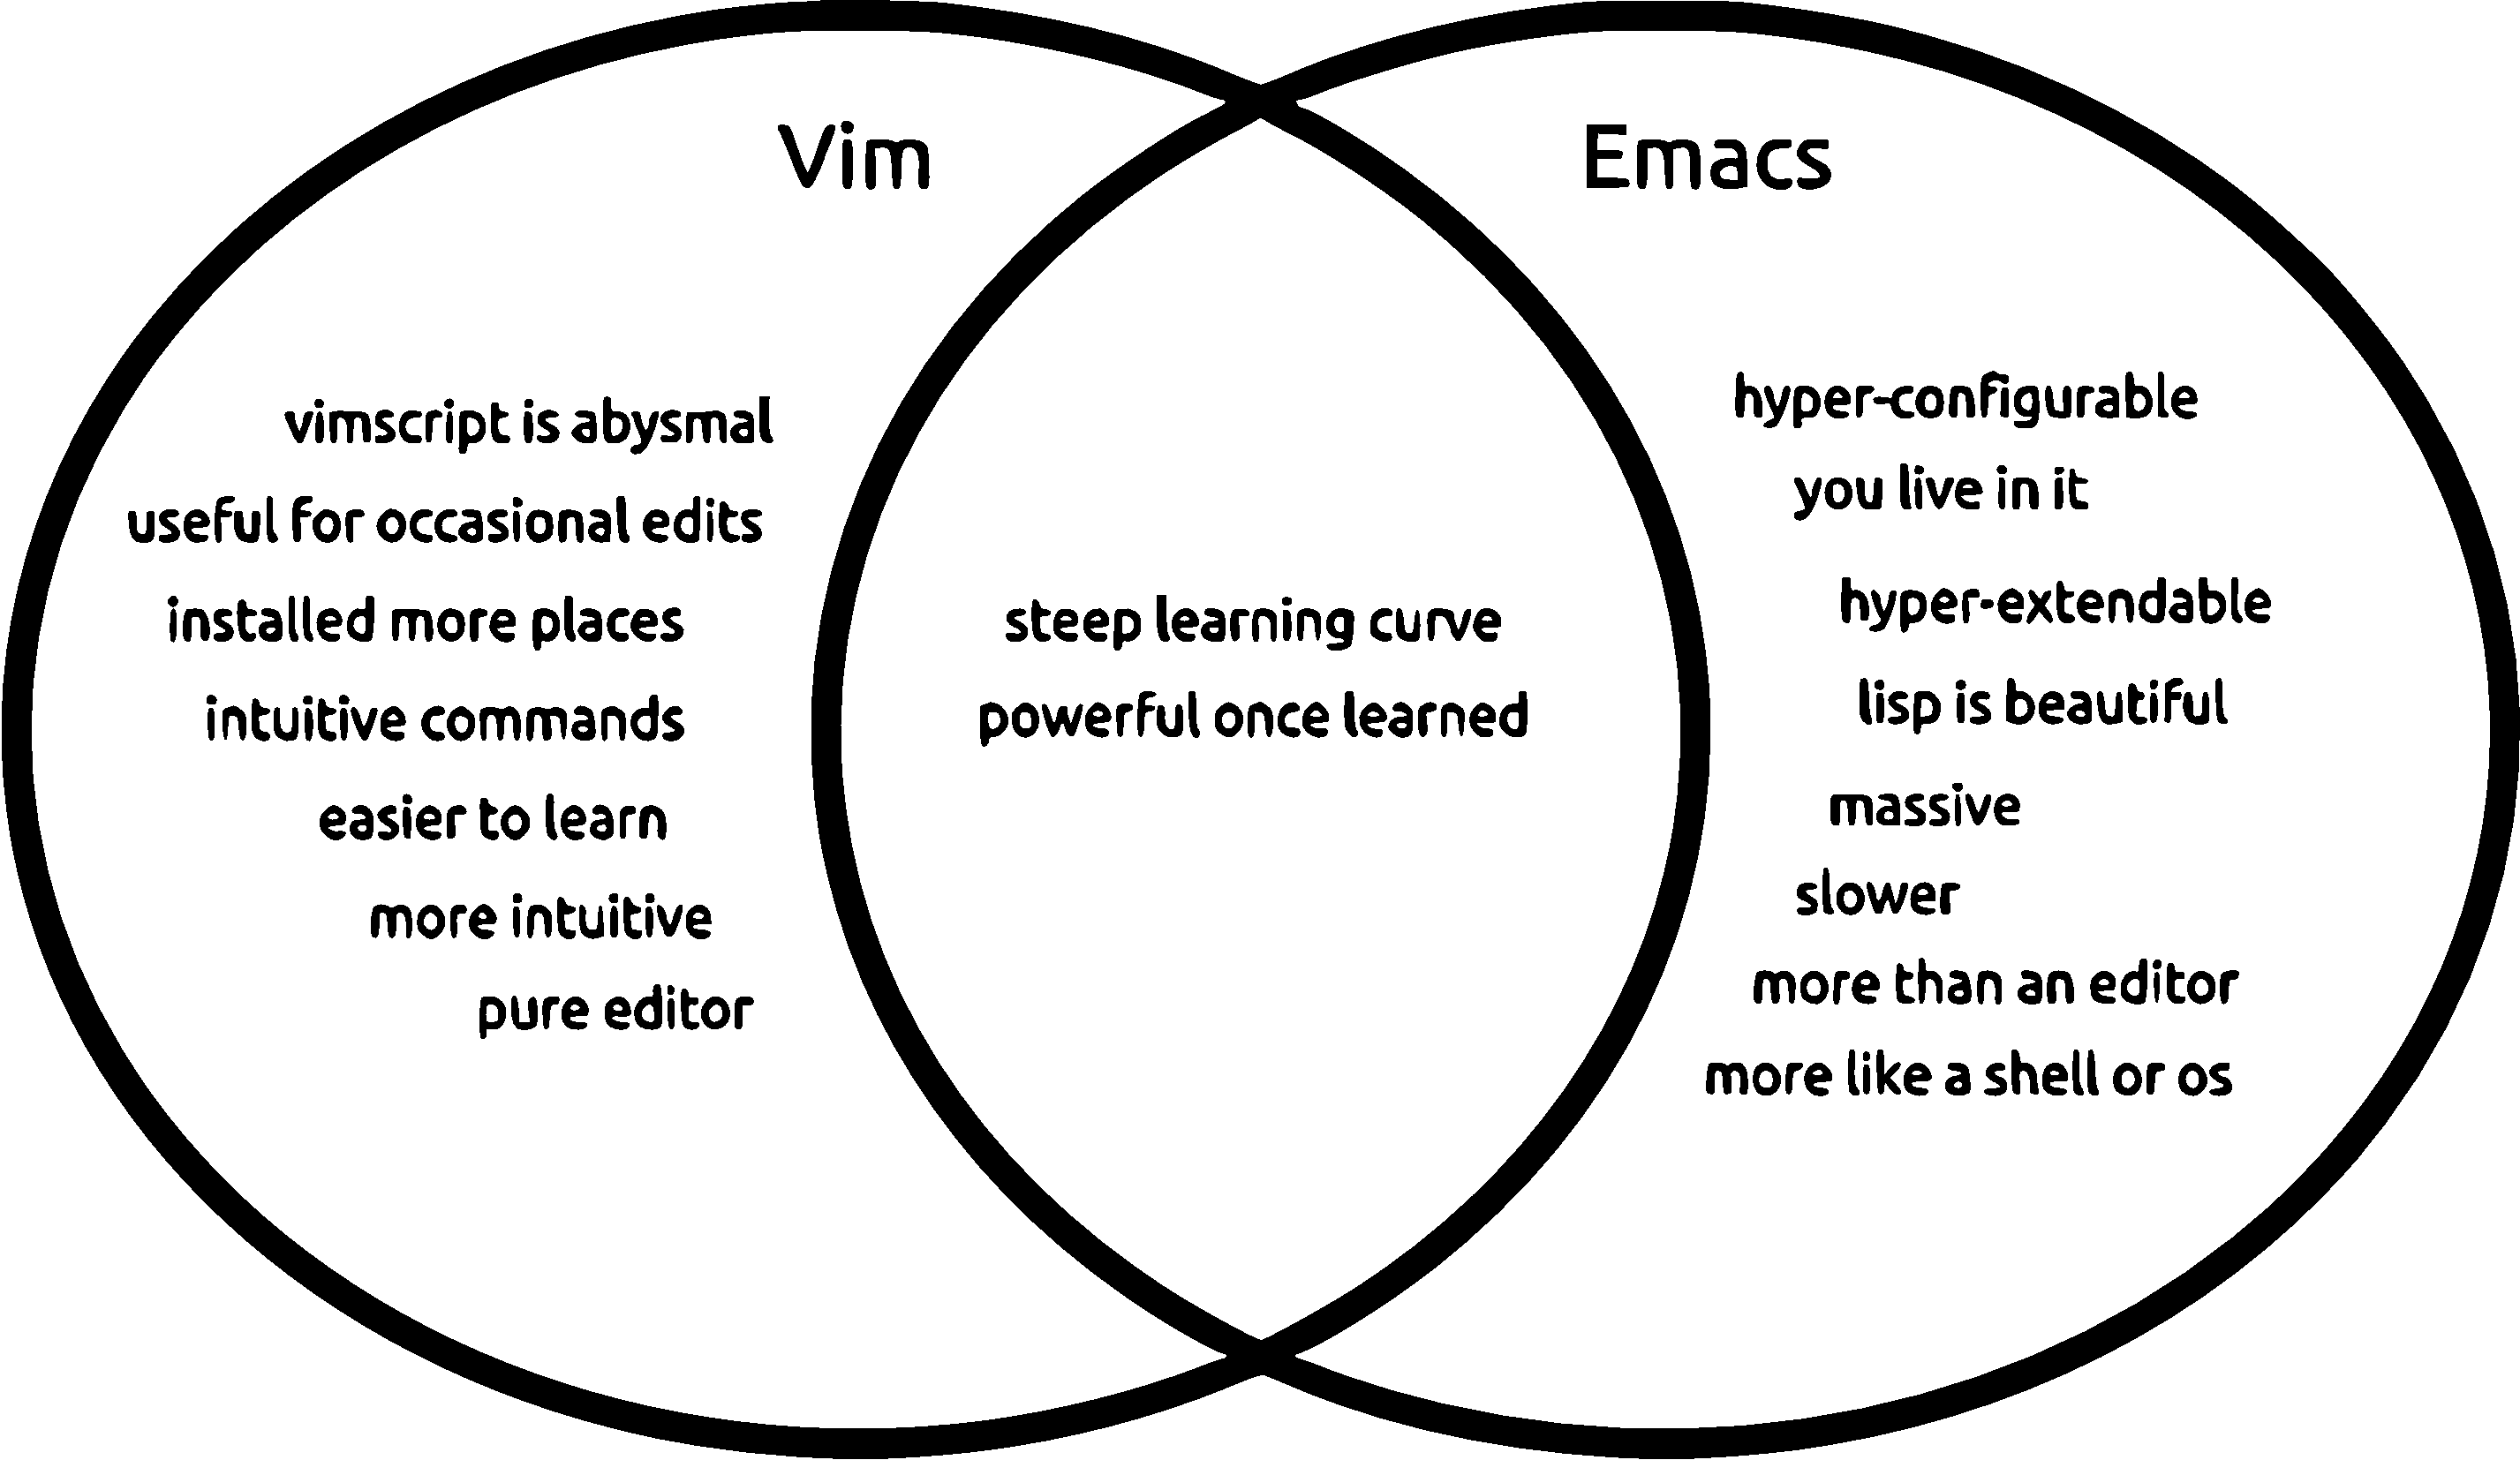
\includegraphics[width=\textwidth]{vivsemacs} }%
      \mode<article>{ 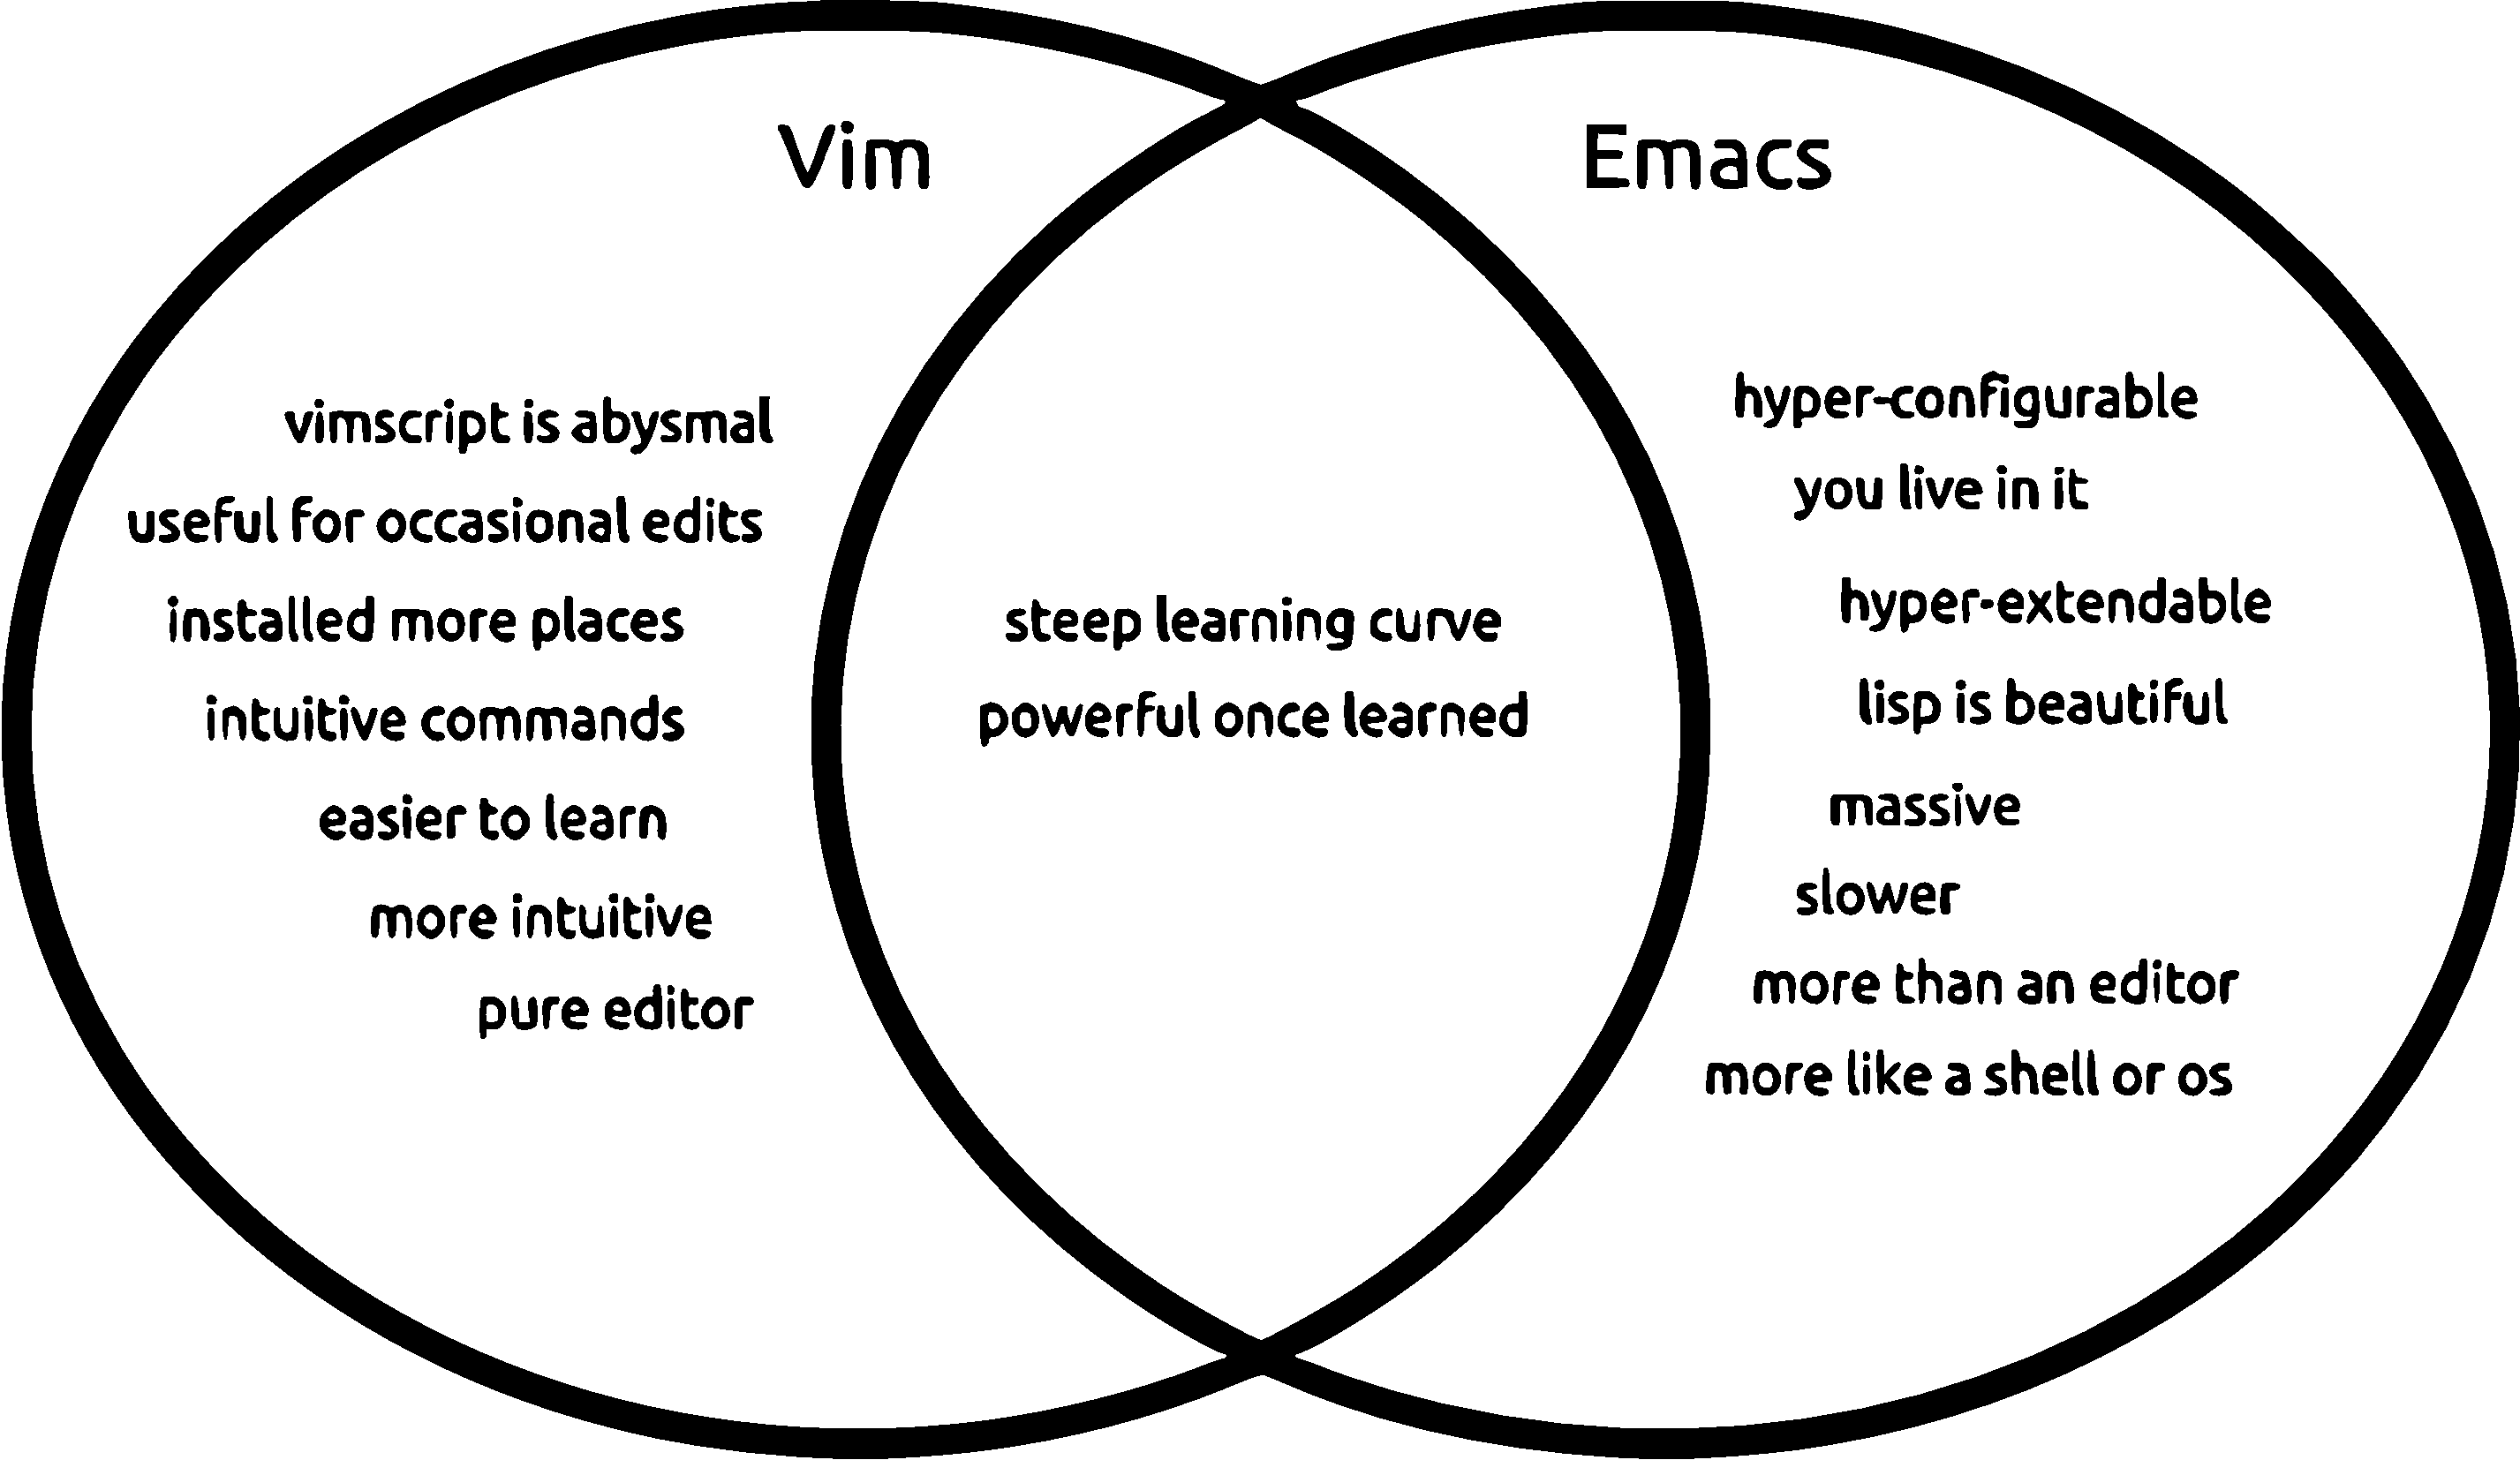
\includegraphics[width=.5\textwidth]{vivsemacs} }
    \end{center}
  \end{block}
\end{frame}

\begin{frame}{Help Your Editor}
  \begin{block}{Suffix matters}\ttfamily
    \begin{itemize}
    \item[\$] vim \wrong
    \item[\$] vim hello \wrong
    \item[\$] vim hello.c  \correct
    \item[\$] vim hello.py \correct
    \item[\$] emacs \wrong
    \item[\$] emacs hello \wrong
    \item[\$] emacsclient hello.c  \correct
    \item[\$] emacsclient hello.py \correct
    \end{itemize}
  \end{block}
\end{frame}

\begin{frame}{Keyboard}
  \begin{center}
    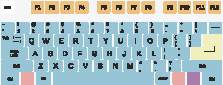
\includegraphics[width=.7\linewidth]{qwerty}
  \end{center}
  \begin{itemize}
  \item[\vim] vimtutor
  \item[\emacs] \Ch{} {\kbd t}
  \end{itemize}
\end{frame}

\section{Shell Basics}
\label{sec:basic-commands}

\begin{frame}{Shell}
  \begin{itemize}
  \item[\shell] A command line interpreter
  \item[\shell] A programming language
  \end{itemize}
  \begin{center}
    \mode<beamer>{ 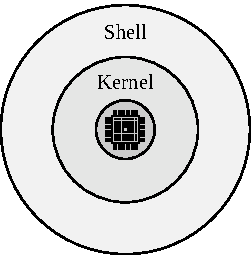
\includegraphics[width=.5\textwidth]{sys-arch} }%
    \mode<article>{ 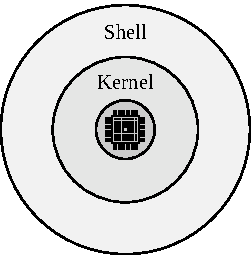
\includegraphics[width=.2\textwidth]{sys-arch} }
  \end{center}
\end{frame}

\begin{frame}{Directory Structure}
  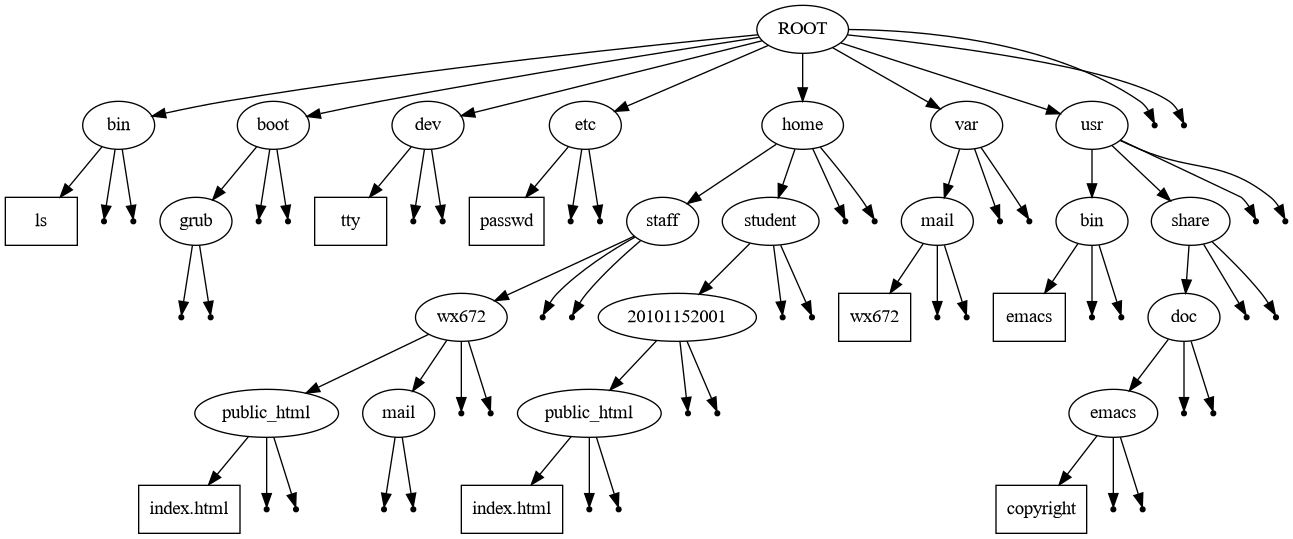
\includegraphics[width=\linewidth]{cs2}
  
  \begin{center}\small
    \begin{tabular}{r@{\qquad}>{\ttfamily}l}
      \hline
      \thead{Todo}  & \thead{How}  \\\hline
      Where am I?   & pwd          \\
      What's in it? & ls           \\
      Move around?  & cd           \\
      Disk usage?   & du, df       \\
      USB drive?    & lsblk, mount \\
      New folder?   & mkdir        \\
      \hline
    \end{tabular}
  \end{center}
\end{frame}

\begin{frame}{File Operations}
  \begin{block}{Ways to create a file}
    \begin{itemize}
    \item[\vim] Using an editor (vim, emacs, nano\ldots), or
    \item[\$] \cmd{cat > filename}
    \item[\$] \cmd{echo "hello, world" > filename}
    \item[\$] \cmd{touch filename}
    \end{itemize}
  \end{block}
  More file operations:
  \begin{center}\small
    \begin{tabular}{r@{\quad}>{\ttfamily}l|r@{\quad}>{\ttfamily}l}
      \hline
      \thead{Todo} & \thead{How} & \thead{Todo} & \thead{How}         \\\hline
      Copy?        & cp          & Move/Rename? & mv                  \\
      Delete?      & rm          & What's it?   & file                \\
      Link?        & ln          & Permission?  & chmod, chown        \\
      Count?       & wc          & Archive?   & tar, gzip, 7z, \ldots \\
      Sort?        & sort, uniq  & Search?      & find, grep          \\
      \hline
    \end{tabular}
  \end{center}
\end{frame}

\begin{frame}{Redirection}
  \begin{block}{Redirecting output}\ttfamily
    \begin{itemize}
    \item[\$] ls -l > output.txt
    \item[\$] ps aux >> output.txt
    \end{itemize}
  \end{block}
  \begin{block}{Redirecting input}\ttfamily
    \begin{itemize}
    \item[\$] more < output.txt
    \end{itemize}
  \end{block}
\end{frame}

\begin{frame}{Process Operations}
  \begin{center}\small
    \begin{tabular}{r@{\quad}>{\ttfamily}l|r@{\quad}>{\ttfamily}l}
      \hline
      \thead{Todo} & \thead{How} & \thead{Todo} & \thead{How}         \\\hline
      Kill?&kill, Ctrl-c&suspend?&Ctrl-z\\
      background?&bg, \& &forground?&fg, jobs\\
      status?&ps, top&&\\\hline
    \end{tabular}
  \end{center}
\end{frame}

\begin{frame}{System Info}
  \begin{center}\small
    \begin{tabular}{r@{\quad}>{\ttfamily}l|r@{\quad}>{\ttfamily}l}
      \hline
      \thead{Todo}   & \thead{How}         & \thead{Todo} & \thead{How}  \\\hline
      who?           & w, who, whoami      & how long?    & uptime       \\
      software?      & apt, aptitude, dpkg & kernel?      & uname, lsmod \\
      hardware?      & lspci, lsusb, lscpu & memory?      & free, lsmem  \\\hline
    \end{tabular}
  \end{center}
  \begin{block}{APT --- ~\debian~package management}
    \begin{center}\small
      \begin{tabular}{l>{\ttfamily}l}
        \hline
        \thead{Todo} & \thead{How}                                       \\\hline
        upgrading?   & apt update \&\& apt upgrade                       \\
        install?     & apt install xxx                                   \\
        remove?      & apt purge xxx                                     \\
        search?      & apt search xxx                                    \\
        details?     & apt show xxx                                      \\
        friendly UI? & aptitude                                          \\\hline
      \end{tabular}
    \end{center}
  \end{block}
\end{frame}

\begin{frame}{CLI Shortcuts}
  \begin{center}
    \begin{tabular}{>{\ttfamily}r@{\quad}l|>{\ttfamily}r@{\quad}l}
      \Ca: & beginning of line  & \Ce:  & end of line      \\
      \Cf: & forward            & \Cb:  & backward         \\
      \Cn: & next               & \Cp:  & previous         \\
      \Cr: & reverse search     & \Cu:  & cut to beginning \\
      \Ck: & kill (cut to end)  & \Cy:  & yank (paste)     \\
      \Cd: & delete a character & \Tab: & completion       \\
    \end{tabular}
  \end{center}
  \begin{block}{Tmux}
    \begin{center}
    \begin{tabular}{>{\ttfamily}r@{\quad}l|>{\ttfamily}r@{\quad}l}
      \Ca {\kbd c}:  & create window      & \Ca \Ca: & switch window    \\
      \Ca {\kbd n}:  & next window        & \Ca {\kbd p}:   & previous window  \\
      \Ca {\kbd -}:  & split window       & \Ca {\kbd |}:   & split widnow     \\
      \Ca {\kbd j}:  & go down            & \Ca {\kbd k}:   & go up            \\
      \Ca {\kbd l}:  & go right           & \Ca {\kbd h}:   & go left          \\
    \end{tabular}
    \end{center}
  \end{block}
\end{frame}

\begin{frame}{Understanding ``\texttt{ls -l}''}
  \begin{minipage}{.71\linewidth}
    \begin{center}
      \mode<beamer>{ 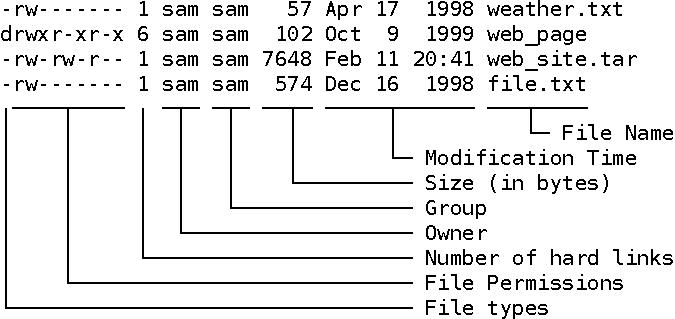
\includegraphics[width=\textwidth]{ls-l} }%
      \mode<article>{ 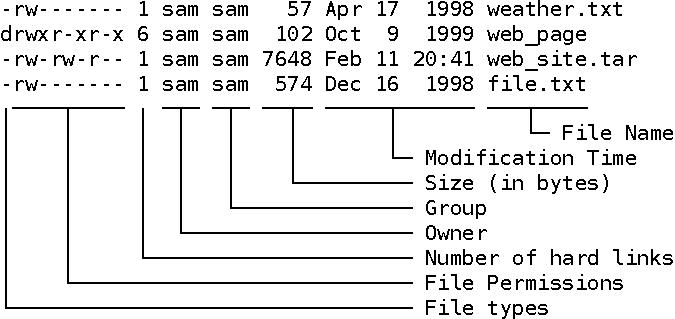
\includegraphics[width=.7\textwidth]{ls-l} }
    \end{center}
  \end{minipage}\quad
  \begin{minipage}{.25\linewidth}\scriptsize
    \begin{tabular}{c@{\;-\;}l}
      d& directory\\
      -& regular file\\
      l& soft link\\
      c& character device\\
      b& block device\\
      s& socket\\
      p& named pipe (FIFO)
      \end{tabular}
  \end{minipage}

  \begin{block}{9-bit permission}
    \begin{minipage}{.27\linewidth}
      \begin{center}
        \mode<beamer>{ 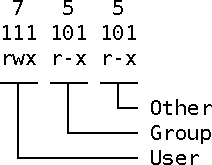
\includegraphics[width=\textwidth]{9bit} }%
        \mode<article>{ 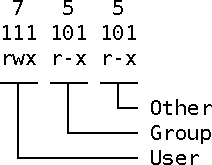
\includegraphics[width=.6\textwidth]{9bit} }
      \end{center}
    \end{minipage}\quad
    \begin{minipage}{.5\linewidth}\small
      \begin{tabular}{l@{\qquad}l}
        \CMD{chmod 755 foo}&\CMD{chmod 644 foo}\\
        \CMD{chmod 000 foo}&\CMD{chmod 777 foo}\\
        \CMD{chmod a-r foo}&\CMD{chmod u+x foo}\\
        \CMD{chmod g+w foo}&\CMD{chmod go=rx foo}
      \end{tabular}
    \end{minipage}
  \end{block}
\end{frame}

\begin{frame}{Wildcard Expansion}
  \begin{center}
    \begin{tabular}{>{\ttfamily}rl>{\ttfamily}l}
      \hline
      \thead{Character}&\thead{Meaning}&\thead{Example}\\\hline
      ?&any one&\CMD{ls ???.txt}\\
      *&zero or more&\CMD{ls *.c}\\
      {[]}&or&\CMD{ls *.[ch]}\\
      \{\}&and&\CMD{ls *.\{c,h,cpp\}}\\\hline    
    \end{tabular}
  \end{center}
  \begin{block}{Example}
    \CMD{touch \{2,3,4,234\}.\{jpg,png\} \&\& ls}\\[1ex]
    \begin{description}
    \item[output:]
      \begin{tabular}{*{4}{>{\ttfamily}r}}\hline
        2.jpg&234.jpg&3.jpg&4.jpg\\
        2.png&234.png&3.png&4.png\\\hline
      \end{tabular}
    \end{description}
    \vspace*{1ex}
    \begin{multicols}{2}
      \begin{itemize}
      \item[\$] \cmd{rm [234].jpg}
      \item[\$] \cmd{rm \{2,3,4,234\}.jpg}
      \item[\$] \cmd{rm 2*}
      \item[\$] \cmd{rm ?.jpg}
      \item[\$] \cmd{rm ?.*}
      \item[\$] \cmd{rm *}
      \end{itemize}
    \end{multicols}
  \end{block}
\end{frame}

\begin{frame}{Everything Is A File}
  \begin{itemize}
  \item[\$] \cmd{cat /dev/null > /var/log/messages \# empty a file}
    \begin{itemize}
    \item[\$] \cmd{: > /var/log/messages \# no new process}
    \end{itemize}
  \item[\$] \cmd{ls > /dev/null}
  \item[\$] \cmd{dd if=/dev/zero of=/tmp/clean bs=1k count=1k}
  \item[\$] \cmd{dd if=/dev/urandom of=/tmp/random bs=1k count=1k}
  \end{itemize}
\end{frame}

\begin{frame}{\texttt{/proc}}
  Allow higher-level access to driver and kernel information
  \ttfamily
  \begin{itemize}
  \item[\$] cat /proc/cpuinfo
  \item[\$] cat /proc/meminfo
  \item[\$] cat /proc/version
  \item[\$] cat /proc/1/status
  \item[\#] echo 100000 > /proc/sys/kernel/pid\_max
  \end{itemize}
\end{frame}

\begin{frame}{Pipe}{Chain processes together}
  \begin{itemize}
  \item[\$] \cmd{ls | wc -l}
  \end{itemize}
  \begin{center}
    \mode<beamer>{ 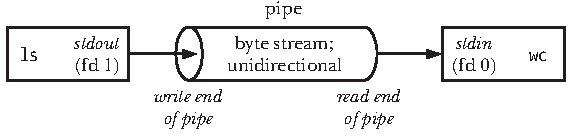
\includegraphics[width=.7\textwidth]{pipe-ls-wc} }%
    \mode<article>{ 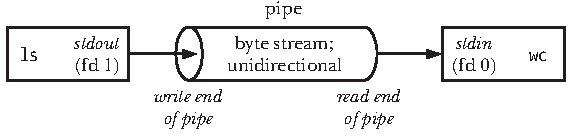
\includegraphics[width=.6\textwidth]{pipe-ls-wc} }
  \end{center}
  \begin{description}
  \item[Unnamed pipe] \,\\
    \CMD{unicode skull | head -1 | cut -f1 -d' ' | sm -}
  \item[Named pipe] \,\\
    \begin{enumerate}
    \item \CMD{mkfifo mypipe}
    \item \CMD{gzip -9 -c < mypipe > out.gz}
    \item \CMD{cat file > mypipe}
    \end{enumerate}
  \end{description}
\end{frame}

\begin{itemize}
\item \url{https://en.wikipedia.org/wiki/Named_pipe}
\end{itemize}

\section{Shell Programming}
\label{sec:shell-programming}

\begin{frame}{\$ --- Give Me The Value Of \ldots}
  \begin{description}
  \item[\texttt{\$var}] Give me the value of variable ``\texttt{var}''
  \item[\texttt{\$(echo hello)}] Give me the value (output) of command ``\cmd{echo hello}''
  \item[\texttt{\$((1+1))}] Give me the value (result) of ``1+1''
  \item[\texttt{\$\$}] Give me the value of special variable ``\texttt{\$}''
  \item[\texttt{\$?}] Give me the value of special variable ``\texttt{?}''
  \item[\texttt{\$0}] Give me the value of special variable ``\texttt{0}''
  \item[\texttt{\$@}] Give me the value of special variable ``\texttt{@}''
  \end{description}
\end{frame}

\begin{frame}{Variables}\ttfamily\small
  \begin{itemize}
  \item[\$] a=8; b=2
  \item[\$] a=a+5; a=\$a+5 \Bad
  \item[\$] let a=a+5; let a+=5 \Good
  \item[\$] let b=b+a; let b+=a \Good
  \item[\$] echo a; echo \$a
  \item[\$] (( a=5, b=6, a+=b )) \Good
  \item[\$] (( b=a<5?8:9 )) \Good
  \item[\$] r=\$(( RANDOM\%100 )) \Good
  \item[\$] echo "\$a" \# partial quoting
  \item[\$] echo '\$a' \# full quoting
  \item[\$] a=\$(ls -l); echo \$a; echo "\$a"
  \item[\$] a=hello; b=world; let a+=b \Bad
  \end{itemize}
\end{frame}

\begin{frame}{Positional Parameters}{\cmd{\$0, \$1, \$2, \ldots, \$@, \$\#}}
  \begin{minipage}{.44\linewidth}
    \begin{center}
      \mode<beamer>{ 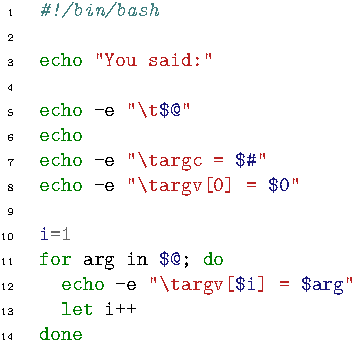
\includegraphics[width=\textwidth]{isay-sh} }%
      \mode<article>{\shellfile{../src/isay.sh}}
    \end{center}
  \end{minipage}\quad
  \begin{minipage}{.52\linewidth}
    \begin{center}
      \mode<beamer>{ 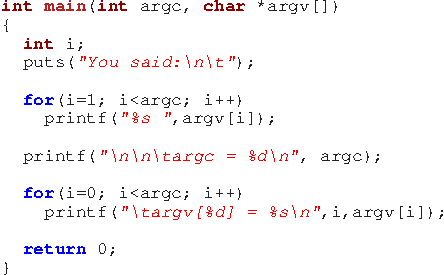
\includegraphics[width=\textwidth]{isay-c} }%
      \mode<article>{\cfile{../src/isay.c}}
    \end{center}
  \end{minipage}
\end{frame}

\begin{frame}{Parameter Substitution}
  \begin{block}{Default value}\ttfamily
    \begin{multicols}{2}
      \begin{itemize}
      \item[\$] echo \$\{s:=abc\}
      \item[\$] echo \$\{s:=xyz\}
      \item[\$] echo \$\{v:-8\}
      \item[\$] echo \$\{v:-10\}
      \end{itemize}
    \end{multicols}
  \end{block}
  \begin{block}{Example}
    \begin{center}
      \mode<beamer>{ 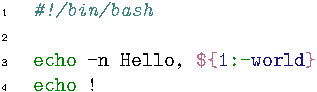
\includegraphics[width=.6\textwidth]{para-substitution-sh} }%
      \mode<article>{\shellfile{../src/para-substitution.sh}}
    \end{center}
  \end{block}
  \begin{itemize}
  \item[\hw] Re-write it in C
  \end{itemize}
\end{frame}
\begin{itemize}
\item[\$] \cmd{sudo apt install abs-guide}
\item \url{file:///usr/share/doc/abs-guide/html/parameter-substitution.html}
\end{itemize}

\begin{frame}{Parameter Substitution}
  \begin{block}{Substring removal}
    \CMD{for f in *.pbm; do ppm2tiff \$f \$\{f\%pbm\}tif; done}
  \end{block}
  \begin{block}{Substring replacement}
    \CMD{for f in *.jpg; do mv \$f \$\{f/jpg/JPG\}; done}
  \end{block}  
\end{frame}

\begin{frame}{Environmental Variables}\ttfamily
  \begin{block}{Each process has an environment}
    \begin{center}\small
      \begin{tabular}{lllll}
        \$PATH&\$PWD&\$HOME&\$UID&\$USER\\
        \$GROUPS&\$SHELL&\$TERM&\$DISPLAY&\$TEMP\\
        \$HOSTNAME&\$HOSTTYPE&\$IFS&\$EDITOR&\$BROWSER\\
        \$HISTSIZE&\$FUNCNAME&\$TMOUT&\ldots&\\
      \end{tabular}
    \end{center}
    \begin{itemize}
    \item[\$] export HISTSIZE=2000
    \item[\$] export BROWSER='/usr/bin/x-www-browser'
    \item[\$] export EDITOR='vim'
    \item[\$] export ALTERNATE\_EDITOR="vim"
    \item[\$] export PDFVIEWER='/usr/bin/zathura'
    \end{itemize}
  \end{block}
  \begin{itemize}
  \item[\$] env
  \item[\$] declare
  \end{itemize}
\end{frame}

\begin{frame}[allowframebreaks]{Tests}\small\ttfamily
  \begin{itemize}
  \item[\$] (( 5 < 6 )) \&\& echo should be
  \item[\$] [[ 1 < 2 ]] \&\& echo of course
  \item[\$] [[ \$a -lt \$b ]] \&\& echo yes || echo no
  \item[\$] if [[ \$a -lt \$b ]]; then echo yes; else echo no; fi
  \item[\$] if test \$a -lt \$b; then echo of course; fi
  \item[\$] if a = 5; then echo a=\$a; fi \# whitespace matters \wrong
  \item[\$] if a=5; then echo a=\$a; fi \Bad
  \item[\$] if test a=5; then echo a=\$a; fi \Bad
  \item[\$] if test a = 5; then echo a=\$a; fi \Bad
  \item[\$] if test \$a = 5; then echo a=\$a; fi \correct
  \item[\$] test \$a = 5 \&\& echo a=\$a \correct
  \item[\$] [[ \$a = 5 ]] \&\& echo a=\$a \correct
  \item[\$] [[ cmp a b ]] \&\& echo same file \wrong
  \item[\$] if test cmp a b; then echo same file; fi \wrong
  \item[\$] if cmp a b; then echo same file; fi \correct
  \item[\$] [[ -f \symbol{`~}/.bash\_aliases ]] \&\& . \symbol{`~}/.bash\_aliases
  \item[\$] [[ -x /usr/bin/xterm ]] \&\& /usr/bin/xterm -e tmux \&
  \item[\$] [[ "\$pass" != "\$MYPASS" ]] \&\& echo 'Wrong password!' \&\& exit 1
  \item[\$] help test
  \end{itemize}
  \begin{block}{}
    \begin{center}
      \mode<beamer>{ 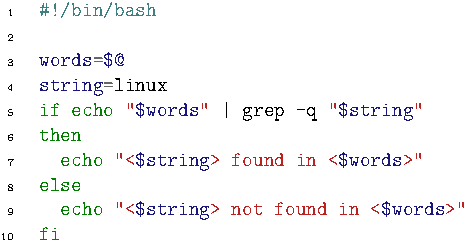
\includegraphics[width=.7\textwidth]{if-then-else-sh} }%
      \mode<article>{\shellfile{../src/if-then-else.sh}}
    \end{center}
  \end{block}
\end{frame}

\begin{frame}{Loops}{\ttfamily for ARG in LIST; do COMMAND(s); done}\small\ttfamily
\begin{itemize}
\item[\$] for i in 1 2 3; do echo -n i="\$i "; done
\item[\$] for i in \{1..10\}; do echo \$i; done
\item[\$] for i in \$(seq 10); do echo \$i; done
\item[\$] for ((i=1; i<=10; i++)); do echo \$i; done
\item[\$] for ((i=1, j=1; i<=10; i++, j++)); do\\
  \quad{}echo \$i-\$j \Bad\\
  \quad{}echo \$((\$i-\$j)) \Good\\
  done
\item[\$] for ((i=1; i<=10; i++)) \{ echo \$i; \} \# C style
\item[\$] for i in hello world; do echo -n "\$i "; done
\end{itemize}
\end{frame}

\begin{frame}{Loops}{\ttfamily while CONDITION; do COMMAND(s); done}\small\ttfamily
\begin{itemize}
\item[\$] a=0; while [[ a < 10 ]]; do echo \$a; ((a++)); done \Bad
\item[\$] while [[ \$a < 10 ]]; do echo \$a; ((a++)); done \Bad
\item[\$] while [[ \$a -lt 10 ]]; do echo \$a; ((a++)); done \correct
\item[\$] while [ \$a -lt 10 ]; do echo \$a; ((a++)); done \correct
\item[\$] while (( a < 10 )); do echo \$a; ((a++)); done \correct
\item[\$] until (( a = 10 )); do echo \$a; ((a++)); done \Bad
\item[\$] until (( a == 10 )); do echo \$a; ((a++)); done \correct
\item[\$] while read n; do n2 \$n; done
\item[\$] while read n; do n2 \$n; done < datafile
\item[\$] until (( n == 0 )); do read n; n2 \$n; done
\end{itemize}
\end{frame}

\begin{frame}{\texttt{case}}
  \begin{center}
    \mode<beamer>{ 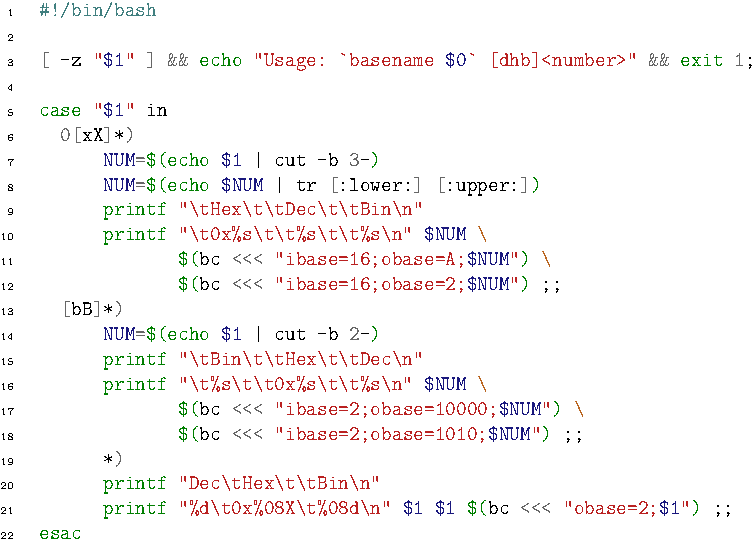
\includegraphics[width=.8\textwidth]{n2-sh} }%
    \mode<article>{\shellfile{../src/n2.sh}}
  \end{center}
\end{frame}

\begin{frame}{\texttt{select}}
  \begin{center}
    \mode<beamer>{ \includegraphics[width=\textwidth]{select-sh} }%
    \mode<article>{\shellfile{../src/select.sh}}
  \end{center}
\end{frame}

\begin{frame}{Functions}
  \mode<beamer>{ \includegraphics[width=\textwidth]{func-sh} }%
  \mode<article>{\shellfile{../src/func.sh}}
\end{frame}

\begin{frame}{Array}
  \begin{center}
    \mode<beamer>{ 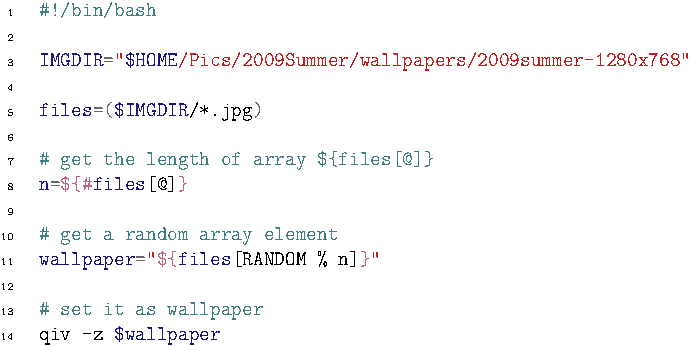
\includegraphics[width=\textwidth]{wallpaper-sh} }%
    \mode<article>{\shellfile{../src/wallpaper.sh}}
  \end{center}
  \begin{itemize}
  \item[\hw] Change wallpaper every 5 mins?
  \end{itemize}
\end{frame}

\begin{itemize}
\item \url{https://www.tutorialspoint.com/unix/unix-using-arrays.htm}
\end{itemize}

\lecture{C Programming Basics}{C basics}
\section{C Programming Basics}
\label{sec:c-programming-basics}

\subsection{Programming Environment}
\label{sec:progr-envir}

\begin{frame}{Program Languages}
  \begin{block}{Machine code}
    The \alert{binary numbers} that the CPUs can understand.
    \begin{center}{\ttfamily
      100111000011101111001111 ... and so on ...}
    \end{center}
    People don't think in numbers.
  \end{block}
  \begin{block}{Assembly language --- friendly to humans}
    \begin{center}
      \mode<beamer>{ \includegraphics[width=.4\textwidth]{asm-sample-asm} }%
      \mode<article>{ \includegraphics[width=.2\textwidth]{asm-sample-asm} }
    \end{center}
    \begin{description}
    \item[Assemblers] translate the ASM programs to machine code
    \end{description}
  \end{block}
\end{frame}

\begin{frame}
  \begin{block}{High level languages}
    Even easier to understand by humans. Examples:
    \begin{itemize}
    \item C\tikzmark{clang}
    \item FORTRAN\tikzmark{fortran}
    \item Java\tikzmark{java}
    \item C++\tikzmark{cpp}
    \item ...\tikzmark{more}
    \end{itemize}\pause
    \begin{description}
    \item[Compilers] do the translation work
    \end{description}
  \end{block}
  \begin{tikzpicture}[remember picture,overlay,
    every node/.style={ellipse,red,opacity=.4,draw},
    every to/.style={append after command={[->,black!30,thick]}}
    ]
    \node (asm) at ($(pic cs:java) + (3,.5ex)$) {Assembly};
    \node (bin) [right=of asm] {Binary};
    \draw ($(pic cs:clang)+(0,.5ex)$) to [bend left=20] (asm);
    \draw ($(pic cs:fortran)+(0,.5ex)$) to [bend left=15] (asm);
    \draw ($(pic cs:java)+(0,.5ex)$) to (asm);
    \draw ($(pic cs:cpp)+(0,.5ex)$) to [bend right=15] (asm);
    \draw ($(pic cs:more)+(0,.5ex)$) to [bend right=20] (asm);
    \draw (asm) to (bin);
    \end{tikzpicture}
\end{frame}

\subsubsection{The Tool Chain}
\label{sec:tool-chain}

\begin{frame}{Compilation}
  \begin{center}
    \mode<beamer>{ \includegraphics[width=\textwidth]{tool-chain} }%
    \mode<article>{ 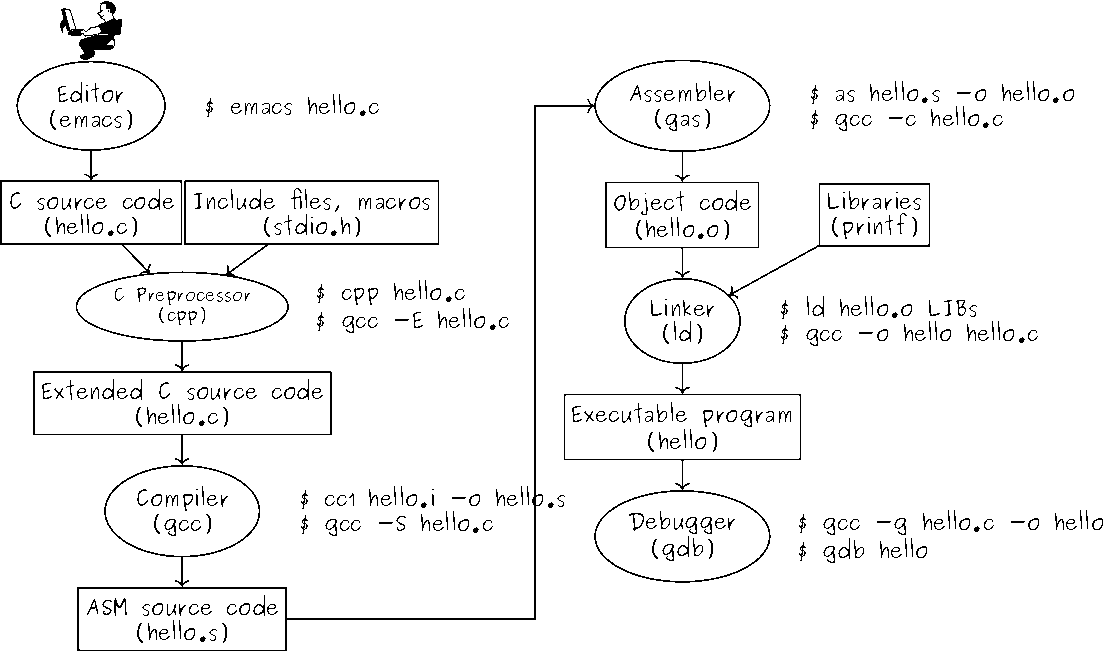
\includegraphics[width=.9\textwidth]{tool-chain-bw} }
  \end{center}
\end{frame}

\begin{description}
\item[Source code] written by programmer in high-level language, in our case in
  \texttt{C}. We write c source code with a \emph{text editor}, such as \texttt{emacs},
  \texttt{vim}, etc.
\item[Preprocessing] is the first pass of any C compilation. It processes
  \texttt{include-files}, \texttt{conditional compilation instructions} and
  \texttt{macros}.
  \begin{description}
  \item[cpp] The GNU C preprocessor
    \begin{itemize}
    \item[\$] \texttt{gcc -E hello.c}
    \end{itemize}
  \end{description}
\item[{Compilation}] is the second pass. It takes the output of the preprocessor, and the
  \texttt{source code}, and generates \texttt{assembly source code}.
  \begin{description}
  \item[gcc/g++] GNU C/C++ compiler
    \begin{itemize}
    \item[\$] \texttt{gcc -S hello.c}
    \end{itemize}
  \end{description}
\item[Assembly] is the third stage of compilation. It takes the assembly source code and
  produces an assembly listing with offsets. The assembler output is stored in an
  \texttt{object file}.
  \begin{description}
  \item[as] the portable GNU assembler
    \begin{itemize}
    \item[\$] \texttt{gcc -c hello.c}
    \end{itemize}
  \end{description}
\item[Linking] is the final stage of compilation. It combines object code with predefined
  routines from \texttt{libraries} and produces the \texttt{executable program}.
  \begin{description}
  \item[ld] The GNU linker
    \begin{itemize}
    \item[\$] \texttt{gcc hello.c -lm}
    \end{itemize}
  \end{description}
\item[{Wrapper}] The whole compilation process is usually not done `by hand', but using a
  \texttt{wrapper} program that combines the functions of preprocessor(cpp),
  compiler(gcc/g++), assembler(as) and linker(ld).
  \begin{itemize}
  \item[\$] \texttt{gcc -Wall hello.c -lm -o hello}
  \end{itemize}
\end{description}

\begin{frame}[fragile]{Compiler vs. Interpreter}
  \begin{block}{\texttt{hello.c}}
    \begin{minipage}{.5\linewidth}
\begin{ccode}
#include <stdio.h>
int main()
{
  printf("Hello, world!\n");
  return 0;
}
\end{ccode}
    \end{minipage}
    \begin{minipage}{.45\linewidth}
    \begin{itemize}
    \item[\$] \texttt{gcc -o hello hello.c}
    \item[\$] \texttt{./hello}
    \end{itemize}
    \end{minipage}
    %\textcolor{LightGray}{\rule{.3\textwidth}{1pt}}
  \end{block}
  \begin{block}{\texttt{hello.sh}}
    \begin{minipage}{.5\linewidth}
      \begin{shellcode}
        #!/bin/bash
        echo 'Hello, world!'
      \end{shellcode}
    \end{minipage}
    \begin{minipage}{.45\linewidth}
      \begin{enumerate}
      \item[\$] \texttt{chmod +x hello.sh}
      \item[\$] \texttt{./hello.sh}
      \end{enumerate}
    \end{minipage}
  \end{block}
  \begin{block}{\texttt{hello.py}}
    \begin{minipage}{.5\linewidth}
\begin{pythoncode}
#!/usr/bin/python
print "Hello, world!"
\end{pythoncode}      
    \end{minipage}
    \begin{minipage}{.45\linewidth}
      \begin{enumerate}
      \item[\$] \texttt{chmod +x hello.py}
      \item[\$] \texttt{./hello.py}
      \end{enumerate}
    \end{minipage}
  \end{block}
\end{frame}

\subsubsection{Header Files}
\label{sec:header-files}

\begin{frame}[fragile]{Header Files}
  \begin{minipage}{.45\linewidth}
    \begin{block}{Why?}
\begin{ccode}
#include "add.h"

int triple(int x)
{
  return add(x, add(x,x));
}
\end{ccode}
    \end{block}
  \end{minipage}\qquad
  \begin{minipage}{.45\linewidth}
    \begin{block}{Why not?}
\begin{ccode}
int add(int, int);

int triple(int x)
{
  return add(x, add(x, x));
}
\end{ccode}
    \end{block}
  \end{minipage}\\[1ex]
  \begin{itemize}
  \item Ensure everyone use the same code
  \item Easy to share, upgrade, reuse
  \end{itemize}
  \begin{block}{In the header files\ldots}
    \begin{multicols}{2}
      \begin{itemize}
      \item function declarations
      \item macro definitions
      \item contants
      \item system wide global variables
      \end{itemize}
    \end{multicols}
  \end{block}
  \begin{itemize}
  \item[\$] \texttt{ls /usr/include/}
  \end{itemize}
\end{frame}

\subsubsection{Library Files}
\label{sec:library-files}

\begin{frame}{Library Files}
  \begin{description}
  \item[Static libraries] \alert{\texttt{.a}} files. Very old ones, but still alive.
    \begin{itemize}
    \item[\$] \texttt{find /usr/lib -name "*.a"}
    \end{itemize}
  \item[Shared libraries] \alert{\texttt{.so}} files. The preferred ones.
    \begin{itemize}
    \item[\$] \texttt{find /usr/lib -name "*.so.*"}
    \end{itemize}
  \end{description}
  Examples:
  \begin{itemize}
  \item[\$] \texttt{gcc -o hello hello.c /usr/lib/libm.a}
  \item[\$] \texttt{gcc -o hello hello.c -lm}
  \end{itemize}
\end{frame}

\begin{frame}
  \begin{block}{Static Linking}
    \begin{itemize}
    \item The entire program and all data of a process must be in physical memory for the
      process to execute
    \item The size of a process is thus limited to the size of physical memory
    \end{itemize}
  \end{block}
    \begin{center}
    \mode<beamer>{ 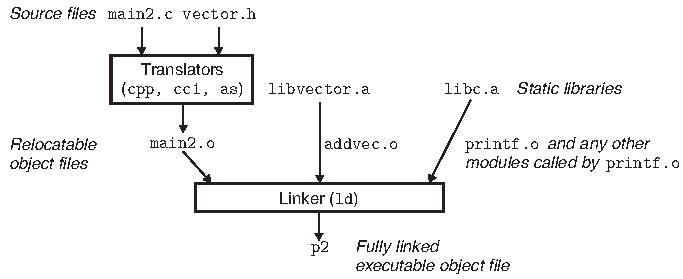
\includegraphics[width=\textwidth]{static-linking} }%
    \mode<article>{ 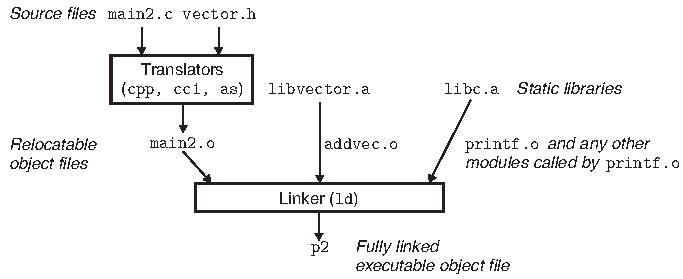
\includegraphics[width=.7\textwidth]{static-linking} }
  \end{center}
\end{frame}

\begin{frame}
  \begin{block}{Dynamic Linking}
    \begin{itemize}
    \item Only one copy in memory
    \item Don't have to re-link after a library update
    \end{itemize}
  \end{block}
  \begin{center}
    \mode<beamer>{ 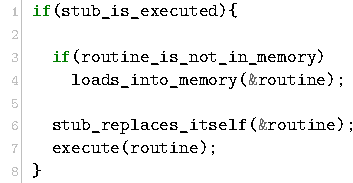
\includegraphics[width=.7\textwidth]{dynamic-linking} }%
    \mode<article>{ 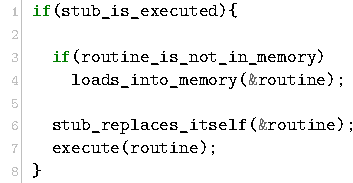
\includegraphics[width=.5\textwidth]{dynamic-linking} }
  \end{center}
\end{frame}

\begin{frame}{Build A Static Library}{Source codes}
  \begin{minipage}[t]{.47\linewidth}
    \begin{block}{\texttt{main.c}}
      \begin{center}
        \mode<beamer>{ \includegraphics[width=\textwidth]{main-c} }%
        \mode<article>{\cfile{../src/static/main.c}}
      \end{center}
    \end{block}
    \begin{block}{\texttt{lib.h}}
      \mode<beamer>{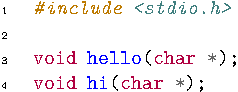
\includegraphics[width=.5\textwidth]{lib-h}}%
      \mode<article>{\cfile{../src/static/lib.h}}
    \end{block}
  \end{minipage}\qquad
  \begin{minipage}[t]{.43\linewidth}
    \begin{block}{\texttt{hello.c}}
      \begin{center}
        \mode<beamer>{ \includegraphics[width=\textwidth]{hello-c} }%
        \mode<article>{\cfile{../src/static/hello.c}}
      \end{center}
    \end{block}
    \begin{block}{\texttt{hi.c}}
      \begin{center}
        \mode<beamer>{ 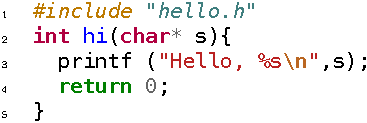
\includegraphics[width=\textwidth]{hi-c} }%
        \mode<article>{\cfile{../src/static/hi.c}}
      \end{center}
    \end{block}
  \end{minipage}
\end{frame}

\begin{frame}{Build A Static Library}{Step by step}
  \begin{enumerate}
  \item Get \alert{\texttt{hello.o}} and \alert{\texttt{hi.o}}
    \begin{itemize}
    \item[\$] \texttt{gcc -c hello.c hi.c}
    \end{itemize}
  \item Put \alert{\texttt{*.o}} into \alert{\texttt{libhi.a}}
    \begin{itemize}
    \item[\$] \texttt{ar crv libhi.a hello.o hi.o}
    \end{itemize}
  \item Use \alert{\texttt{libhi.a}}
    \begin{itemize}
    \item[\$] \texttt{gcc main.c libhi.a}
    \end{itemize}
  \end{enumerate}
\end{frame}

\begin{frame}{Build A Static Library}{Makefile}
  \begin{center}
    \mode<beamer>{ \includegraphics[width=.8\textwidth]{makefile-a} }%
    \mode<article>{\mkfile{../src/static/Makefile}}
  \end{center}
\end{frame}

\begin{frame}{Build A Shared Library}{Source codes}
  \begin{block}{\texttt{hello.c}}
    \begin{center}
      \mode<beamer>{ \includegraphics[width=.8\textwidth]{hello-c-so} }%
      \mode<article>{\cfile{../src/shared/hello.c}}
    \end{center}
  \end{block}
  \begin{minipage}{.35\linewidth}
    \begin{block}{\texttt{hello.h}}
      \mode<beamer>{ \includegraphics[width=\textwidth]{hello-h-so} }%
      \mode<article>{\cfile{../src/shared/hello.h}}
    \end{block}
  \end{minipage}\qquad
  \begin{minipage}{.36\linewidth}
    \begin{block}{\texttt{hi.c}}
      \mode<beamer>{ \includegraphics[width=\textwidth]{hi-c-so} }%
      \mode<article>{\cfile{../src/shared/hi.c}}
    \end{block}
  \end{minipage}
\end{frame}

\begin{frame}{Build A Shared Library}{Step by step}
  \begin{enumerate}
  \item Get \alert{\texttt{hi.o}}
    \begin{itemize}
    \item[\$] \texttt{gcc -fPIC -c hi.c}
    \end{itemize}
  \item Get \alert{\texttt{libhi.so}}
    \begin{itemize}
    \item[\$] \texttt{gcc -shared -o libhi.so hi.o}
    \end{itemize}
  \item Use \alert{\texttt{libhi.so}}
    \begin{itemize}
    \item[\$] \texttt{gcc -L. -Wl,-rpath=. hello.c -lhi}
    \end{itemize}
  \item Check it
    \begin{itemize}
    \item[\$] \texttt{ldd a.out}
    \end{itemize}
  \end{enumerate}
\end{frame}

\begin{frame}{Build A Shared Library}{Makefile}
  \begin{center}
    \mode<beamer>{ \includegraphics[width=\textwidth]{makefile-so} }%
    \mode<article>{\mkfile{../src/shared/Makefile}}
  \end{center}
\end{frame}

\begin{frame}{GNU C Library}
  \begin{minipage}{.55\linewidth}
    Linux API > POSIX API
    \ttfamily
    \begin{itemize}
    \item[\$] man 7 libc
    \item[\$] man 3 intro
    \item[\$] man gcc
    \item[\$] info gcc
    \item[\debian] sudo apt install gcc-doc
    \end{itemize}
  \end{minipage}
  \begin{minipage}{.4\linewidth}
    \begin{center}
      \mode<beamer>{ 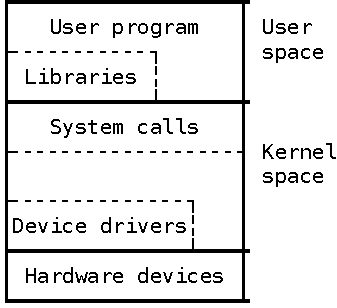
\includegraphics[width=\textwidth]{api} }%
      \mode<article>{ 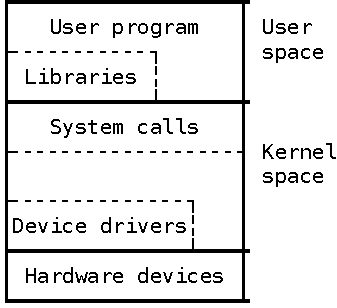
\includegraphics[width=.5\textwidth]{api} }
    \end{center}
  \end{minipage}
\end{frame}

\subsubsection{Error Handling}
\label{sec:error-handling}

\begin{frame}{\texttt{errno.h}}
  \begin{center}
    \mode<beamer>{ 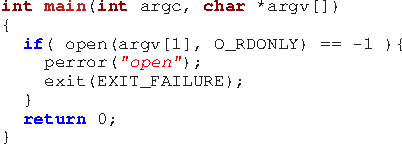
\includegraphics[width=.6\textwidth]{perror-c} }%
    \mode<article>{\cfile{../src/perror.c}}
  \end{center}\ttfamily
  \begin{itemize}
  \item[\$] man errno
  \item[\$] man errno.h
  \item[\$] man perror
  \end{itemize}
\end{frame}

\begin{itemize}
\item \citetitle[Sec.~1.7]{stevens2013advanced}
\item \url{https://stackoverflow.com/questions/30078281/raise-error-in-a-bash-script}
\end{itemize}

\subsubsection{The Make Utility}

\begin{frame}{The Make Utility}
  To compile a single C program:
  \begin{itemize}
  \item[\$] \cmd{gcc hello.c -o hello}\quad{\Huge \correct}\textsubscript{{\tiny OK. But\ldots}}
    % \tikz \node [opacity=.4,red,scale=3,inner
    % sep=0pt,label={[below=2.5ex,right]{\tiny OK. But...}}] {\Checked};
  \end{itemize}
  \begin{block}{What if you have a large project with 1000+ files?}
    \begin{center}
      \mode<beamer>{ 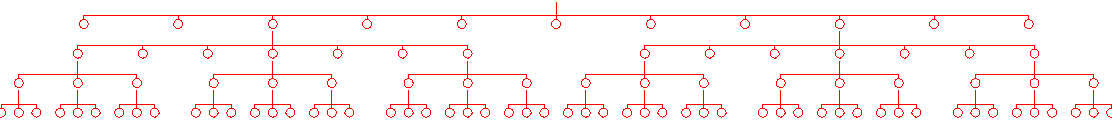
\includegraphics[width=\textwidth]{tree} }%
      \mode<article>{ 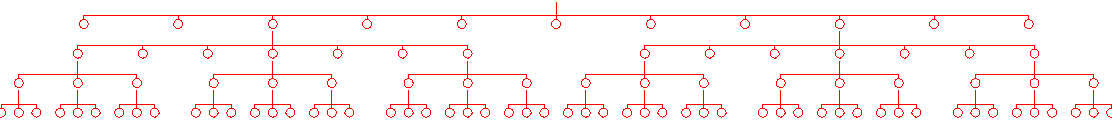
\includegraphics[width=.5\textwidth]{tree} }
    \end{center}
    \begin{description}
    \item[Linux 4.9 source tree:] 3799 directories, 55877 files
    \end{description}
  \end{block}
  \begin{description}
  \item[make:] help you maintain your programs.
  \end{description}
\end{frame}

\begin{frame}{Makefile}
  \begin{block}{}
      \mode<beamer>{ 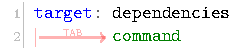
\includegraphics[width=.5\textwidth]{mktab1} }%
      \mode<article>{ 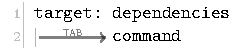
\includegraphics[width=.3\textwidth]{mktab1-bw} }
  \end{block}
  \begin{block}{Example}
      \mode<beamer>{ 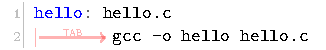
\includegraphics[width=.6\textwidth]{mktab2} }%
      \mode<article>{ 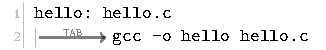
\includegraphics[width=.4\textwidth]{mktab2-bw} }
  \end{block}
  \begin{itemize}
  \item[\$] \cmd{info make makefiles}
  \end{itemize}
\end{frame}

\begin{frame}{Makefile}
  \begin{minipage}{.75\linewidth}
    \mode<beamer>{ 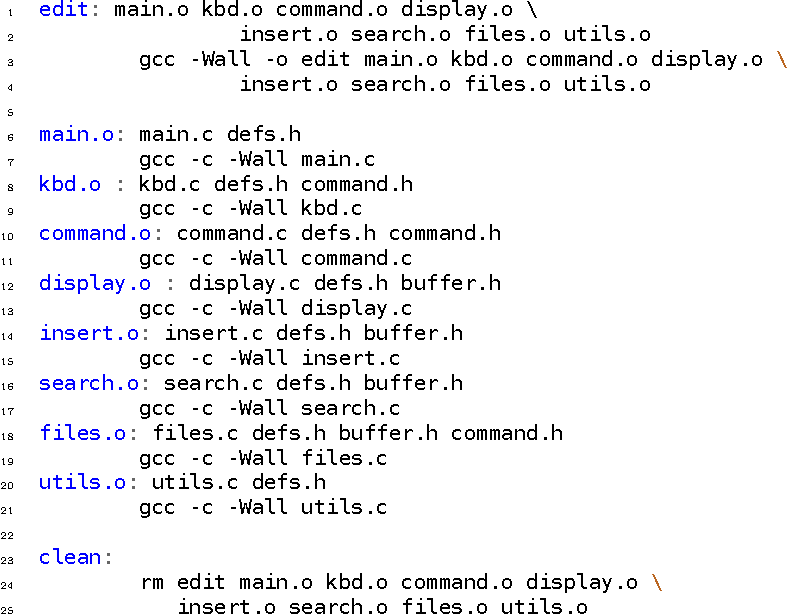
\includegraphics[width=1.1\textwidth]{Makefile2-mk} }%
    \mode<article>{\mkfile{figs/Makefile2}}
  \end{minipage}
  \begin{minipage}{.2\linewidth}
    \begin{center}
      \mode<beamer>{ \includegraphics[width=\textwidth]{make-dir-tree} }%
      \mode<article>{ \includegraphics[width=.7\textwidth]{make-dir-tree} }
    \end{center}
  \end{minipage}
\end{frame}

\subsubsection{Version Control}
\label{sec:version-control}

\begin{frame}{git}
  \begin{block}{To create a new local git repo}
    In your source code directory, do:\ttfamily
    \begin{itemize}
    \item[\$] git init
    \item[\$] git add .
    \item[\$] git commit -m "something to say\ldots"
    \end{itemize}
  \end{block}
  \begin{block}{To clone a remote repo}
    Example:\ttfamily
    \begin{itemize}
    \item[\$] git clone https://github.com/wx672/lecture-notes.git
    \item[\$] git clone https://github.com/wx672/dotfile.git
    \end{itemize}
  \end{block}
\end{frame}

\begin{frame}
  \begin{block}{Most commonly used git Commands}\ttfamily
    \begin{itemize}
    \item[\$] git add filename[s]
    \item[\$] git rm filename[s]
    \item[\$] git commit
    \item[\$] git status\qquad\CMD{git log}\qquad\CMD{git diff}
    \item[\$] git push\qquad\CMD{git pull}
    \item[\$] git help \{add,rm,commit,\ldots\}
    \end{itemize}
  \end{block}
  \begin{multicols}{2}
    \begin{itemize}
    \item[\$] man gittutorial
    \item[\$] man gittutorial-2
    \item[\debian] sudo apt install git
    \item[\github] \url{https://github.com}
    \end{itemize}
  \end{multicols}
\end{frame}

\subsubsection{Manual Pages}
\label{sec:manual-pages}

\begin{frame}{Man page}{Layout}
  \begin{center}
    \mode<beamer>{ \includegraphics[width=.8\textwidth]{manpage-txt} }%
    \mode<article>{ \includegraphics[width=.5\textwidth]{manpage-txt} }
  \end{center}
\end{frame}

\begin{frame}{Man Page}{Groff source code}
  \begin{minipage}[b]{.6\linewidth}
    \begin{center}
      \mode<beamer>{ \includegraphics[width=1.6\textwidth]{manpage-1} }%
      \mode<article>{ \includegraphics[width=1.2\textwidth]{manpage-1-bw} }
    \end{center}
  \end{minipage}
  \begin{minipage}[b]{.35\linewidth}\ttfamily
    \begin{itemize}
    \item[\$] man 7 groff
    \item[\$] man txt2man
    \item[\$] man a2x
    \item[\$] ls /usr/share/man
    \end{itemize}
  \end{minipage}
\end{frame}

\subsubsection{A Sample GNU Package}
\label{sec:sample-gnu-package}

\begin{frame}{How to ``Do one thing, and do it well''?}  
  \begin{itemize}
  \item[\$] \cmd{apt source hello}
  \end{itemize}
\end{frame}

\subsection{OS Basics}
\label{sec:os-basics}

\begin{frame}<beamer>{Operating System}
  \centering
  \includegraphics[height=.85\textheight]{kernel-block}
\end{frame}

\begin{frame}{Abstractions}{To hide the complexity of the actual implementations}
  \begin{center}
    \mode<beamer>{ \includegraphics[width=\textwidth]{abstraction} }%
    \mode<article>{ \includegraphics[width=.5\textwidth]{abstraction} }
  \end{center}
\end{frame}

See also: \citetitle[Sec.~1.9.2, \emph{The Importance of Abstractions in Computer
  Systems}]{Bryant2010computersystems}.

\begin{frame}{A Computer System}
  \begin{center}
    \mode<beamer>{ \includegraphics[width=\textwidth]{mos-figs-1-1} }%
    \mode<article>{ \includegraphics[width=.5\textwidth]{mos-figs-1-1} }
  \end{center}
\end{frame}

\subsubsection{Hardware}
\label{sec:cpu}

\begin{frame}{CPU Working Cycle}
  \begin{center}
    \mode<beamer>{ \includegraphics[width=.6\textwidth]{mos-figs-1-6} }%
    \mode<article>{ \includegraphics[width=.3\textwidth]{mos-figs-1-6} }
  \end{center}
  \begin{enumerate}
  \item Fetch the first instruction from memory
  \item Decode it to determine its type and operands
  \item execute it
  \end{enumerate}
  \begin{block}{Special CPU Registers}
    \begin{description}
    \item[Program counter (PC):] keeps the memory address of the next instruction to
      be fetched
    \item[Stack pointer (SP):] {\symbola ☛} the top of the current stack in memory
    \item[Program status (PS):] holds
      \begin{itemize}
      \item[-] condition code bits
      \item[-] processor state
      \end{itemize}
    \end{description}
  \end{block}
\end{frame}

\begin{frame}{System Bus}
  \begin{center}
    \mode<beamer>{ \includegraphics[width=\textwidth]{mos-figs-1-5} }%
    \mode<article>{ \includegraphics[width=.6\textwidth]{mos-figs-1-5} }
  \end{center}
  \begin{description}
  \item[Address Bus:] specifies the memory locations (addresses) for the
    data transfers
  \item[Data Bus:] holds the data transfered. Bidirectional
  \item[Control Bus:] contains various lines used to route timing and
    control signals throughout the system
  \end{description}
\end{frame}

\begin{frame}{Controllers and Peripherals}
  \begin{itemize}
  \item Peripherals are real devices controlled by controller chips
  \item Controllers are processors like the CPU itself, have control registers
  \item Device driver writes to the registers, thus control it
  \item Controllers are connected to the CPU and to each other by a variety of buses
  \end{itemize}
\end{frame}

\begin{frame}
  \begin{center}
    \mode<beamer>{ \includegraphics[width=\textwidth]{mos-figs-1-11} }%
    \mode<article>{ \includegraphics[width=.6\textwidth]{mos-figs-1-11} }
  \end{center}
\end{frame}

\begin{frame}{Motherboard Chipsets}
  \begin{center}
    \mode<beamer>{ \includegraphics[width=\textwidth]{chipsets} }
    \mode<article>{ \includegraphics[width=.5\textwidth]{chipsets-bw} }
  \end{center}
\end{frame}

See also:
\href{http://duartes.org/gustavo/blog/post/motherboard-chipsets-memory-map}{\emph{Motherboard
    Chipsets And The Memory Map}}
\footnote{\url{http://duartes.org/gustavo/blog/post/motherboard-chipsets-memory-map}}.

\begin{frame}
  \begin{itemize}
  \item The CPU doesn't know what it's connected to
    \begin{itemize}
    \item[-] CPU test bench?\quad{}network router?\quad{}toaster?\quad{}brain implant?
    \end{itemize}
  \item The CPU talks to the outside world through its pins
    \begin{itemize}
    \item[-] some pins to transmit the physical memory address
    \item[-] other pins to transmit the values
    \end{itemize}
  \item The CPU's gateway to the world is the \alert{front-side bus}
  \end{itemize}
  \begin{block}{Intel Core 2 QX6600}
    \begin{itemize}
    \item 33 pins to transmit the physical memory address
      \begin{itemize}
      \item[-] so there are $2^{33}$ choices of memory locations
      \end{itemize}
    \item 64 pins to send or receive data
      \begin{itemize}
      \item[-] so data path is 64-bit wide, or 8-byte chunks
      \end{itemize}
    \end{itemize}
    This allows the CPU to physically address 64GB of memory ($2^{33}\times{}8B$)    
  \end{block}
\end{frame}

See also:
\href{http://download.intel.com/design/processor/datashts/31559205.pdf}{\emph{Datasheet
    for Intel Core 2 Quad-Core Q6000 Sequence}}
\footnote{\url{http://download.intel.com/design/processor/datashts/31559205.pdf}}.

\begin{frame}[plain]
  \begin{minipage}{.65\linewidth}
    \begin{block}{Some physical memory addresses are mapped away!}
      \begin{itemize}
      \item only the addresses, not the spaces
      \item Memory holes
        \begin{itemize}
        \item[-] 640 KiB~\symbol{`~}~1 MiB
        \item[-] \texttt{/proc/iomem}
        \end{itemize}
      \end{itemize}
    \end{block}
    \begin{block}{Memory-mapped I/O}
      \begin{itemize}
      \item BIOS ROM
      \item video cards
      \item PCI cards
      \item \ldots
      \end{itemize}
      This is why 32-bit OSes have problems using 4 GiB of RAM.
    \end{block}
  \end{minipage}\quad
  \begin{minipage}{.3\linewidth}
    \tikz[baseline,overlay]{
      \node [xshift=1.4cm,yshift=-1cm] at (0,0) {
        \includegraphics[scale=0.6]{boot-mem}}}
  \end{minipage}
  % \begin{center}
  %   What if you don't have 4G RAM?
  % \end{center}
\end{frame}

\begin{frame}
  \begin{block}{the northbridge}
    \begin{enumerate}
    \item receives a physical memory request
    \item decides where to route it
      \begin{itemize}
      \item[-] to RAM? to video card? to \ldots{}?
      \item[-] decision made via the \alert{memory address map}
      \end{itemize}
    \end{enumerate}
  \end{block}
\end{frame}

\begin{itemize}
\item When is the memory address map built? \texttt{setup()}.
\end{itemize}

\subsubsection{Bootstrapping}
\label{sec:bootstrapping}

\begin{frame}{Bootstrapping}
  \begin{block}{Can you pull yourself up by your own bootstraps?}
    \begin{itemize}
    \item[] A computer cannot run without first loading software but must be running
      before any software can be loaded.
    \end{itemize}
  \end{block}
  \begin{center}
    \mode<beamer>{ \includegraphics[width=\textwidth]{boot}}%
    \mode<article>{ \includegraphics[width=.7\textwidth]{boot-bw}}
  \end{center}
\end{frame}

\begin{frame}{Intel x86 Bootstrapping}
  \begin{enumerate}
  \item BIOS (\texttt{0xfffffff0})\\
    \begin{small}
      {\Symbol{➠}} POST\quad
      {\Symbol{➠}} HW init\quad
      {\Symbol{➠}} Find a boot device (FD,CD,HD\ldots{})\quad
      {\Symbol{➠}} Copy \alert{sector zero (MBR)} to RAM (\texttt{0x00007c00})
    \end{small}
  \item MBR -- the first 512 bytes, contains
    \begin{itemize}
    \item Small code ($< 446\,B$), e.g. GRUB stage 1, for loading GRUB stage 2
    \item the primary partition table ($16\times{}4=64\,B$)
    \item its job is to load the second-stage boot loader.
    \end{itemize}
  \item GRUB stage 2 --- load the OS kernel into RAM
  \item {\linux} startup
  \item init --- the first user-space process
  \end{enumerate}
  \begin{center}
    \mode<beamer>{ \includegraphics[width=.8\textwidth]{mbr}}%
    \mode<article>{ \includegraphics[width=.5\textwidth]{mbr}}
  \end{center}
  \qquad\CMD{sudo hd -n512 /dev/sda}
\end{frame}

\begin{itemize}
\item \url{https://en.wikipedia.org/wiki/Unified_Extensible_Firmware_Interface}
\end{itemize}

\lecture{Interrupt}{int}
\subsubsection{Interrupt}
\label{sec:interrupt}

\begin{frame}{Why Interrupt?}
  \begin{block}{While a process is reading a disk file, can we do...}
    \begin{center}
      \mode<beamer>{ \includegraphics[width=.6\textwidth]{interrupt}}%
      \mode<article>{ \includegraphics[width=.3\textwidth]{interrupt-bw}}
    \end{center}
  \end{block}
\end{frame}

\begin{frame}{Modern OS are Interrupt Driven}
  \begin{description}
  \item[HW INT] by sending a signal to CPU
  \item[SW INT] by executing a \alert{system call}
  \item[Trap (exception)] is a software-generated INT coursed by an error or by a
    specific request from an user program
  \item[Interrupt vector] is an array of pointers {\pright} the memory addresses
    of \alert{interrupt handlers}. This array is indexed by a unique device number
    \begin{itemize}
    \item[\$] \cmd{less /proc/devices}
    \item[\$] \cmd{less /proc/interrupts}
    \end{itemize}
  \end{description}
\end{frame}

\begin{frame}{Programmable Interrupt Controllers}
  \begin{center}
    \mode<beamer>{ \includegraphics[width=\textwidth]{int-osdi-34}}%
    \mode<article>{ \includegraphics[width=.5\textwidth]{int-osdi-34}}
  \end{center}
\end{frame}

\begin{frame}{Interrupt Processing}
  \begin{center}
    \mode<beamer>{%
      \includegraphics[width=.4\textwidth]{mos-figs-1-10-1}\qquad%
      \includegraphics[width=.3\textwidth]{mos-figs-1-10-2}
    } \mode<article>{%
      \includegraphics[width=.3\textwidth]{mos-figs-1-10-1}\qquad%
      \includegraphics[width=.2\textwidth]{mos-figs-1-10-2}%
    }
  \end{center}
\end{frame}

\begin{itemize}
\item \citetitle[Sec.~1.3.5, \emph{I/O Devices}]{tanenbaum2015modern}
\end{itemize}

\begin{frame}{Interrupt Timeline}
  \begin{center}
    \mode<beamer>{ \includegraphics[width=\textwidth]{ir-timeline} }%
    \mode<article>{ \includegraphics[width=.5\textwidth]{ir-timeline} }
  \end{center}
\end{frame}

\lecture{System Calls}{syscall}
\subsubsection{System Calls}
\label{sec:system-calls}

\begin{frame}{System Calls}
  \begin{block}{A System Call}
    \begin{itemize}
    \item is how a program requests a service from an OS kernel
    \item provides the interface between a process and the OS
    \end{itemize}
  \end{block}
  \begin{itemize}
  \item[\$] \cmd{man 2 intro}
  \item[\$] \cmd{man 2 syscalls}
  \end{itemize}
\end{frame}

\begin{frame}
  \begin{center}
    \mode<beamer>{ \includegraphics[height=\textheight]{syscall} }%
    \mode<article>{ \includegraphics[width=.45\textwidth]{syscall} }
  \end{center}
\end{frame}

\begin{frame}{The 11 steps in making a system call}{\texttt{read(fd,buffer,nbytes)}}
  \begin{center}
    \mode<beamer>{ \includegraphics[width=.8\textwidth]{mos-figs-1-18} }%
    \mode<article>{ \includegraphics[width=.6\textwidth]{mos-figs-1-18} }
  \end{center}
\end{frame}

\begin{frame}{Example}{Linux \texttt{INT 80h}}
  \begin{description}
  \item[Interrupt Vector Table:] The very first 1KiB of x86 memory. 
    \begin{itemize} 
    \item 256 entries $\times$ 4B = 1KiB
    \item Each entry is a complete memory address (\texttt{segment:offset})
    \item It's populated by Linux and BIOS
    \item Slot \texttt{80h}: address of the kernel services dispatcher ({\pright} sys-call table)
    \end{itemize}
  \end{description}
\end{frame}

\begin{frame}{Example}
  \begin{center}
    \mode<beamer>{ \includegraphics[width=.8\textwidth]{h-asm} }%
    \mode<article>{ \includegraphics[width=.4\textwidth]{h-asm-bw} }
  \end{center}
  \begin{block}{}
    \ttfamily
    \begin{enumerate}
    \item[\$] nasm -f elf64 hello.asm -o hello.o
    \item[\$] ld hello.o -o hello
    \item[\$] ./hello
    \end{enumerate}
  \end{block}
\end{frame}

\begin{frame}%{System Calls}
  \begin{center}
    \mode<beamer>{ \includegraphics[width=.75\textwidth]{mos-figs-1-19} }
    \mode<article>{ \includegraphics[width=.7\textwidth]{mos-figs-1-19} }
  \end{center}
\end{frame}

\begin{frame}{System Call Examples}
  \begin{block}{\cmd{fork()}}
    \begin{center}
      \mode<beamer>{ \includegraphics[width=.8\textwidth]{fork} }%
      \mode<article>{ \includegraphics[width=.4\textwidth]{fork-bw} }
    \end{center}
  \end{block}
  \qquad\CMD{man 2 fork}
\end{frame}

\begin{frame}
  \begin{block}{\cmd{execve()}}
    \begin{center}
      \mode<beamer>{ \includegraphics[width=\textwidth]{fork-exec} }%
      \mode<article>{ \includegraphics[width=.7\textwidth]{fork-exec-bw} }
    \end{center}
  \end{block}\ttfamily
  \begin{itemize}
  \item[\$] man 2 execve
  \item[\$] man 3 exec
  \end{itemize}
\end{frame}

Quoted from
\href{https://stackoverflow.com/questions/20823371/what-is-the-difference-between-the-functions-of-the-exec-family-of-system-calls}{
  stackoverflow: What is the difference between the functions of the \emph{exec} family of system calls}:

\begin{quote}
  There is no \emph{exec} system call --- this is usually used to refer to all the
  \emph{execXX} calls as a group. They all do essentially the same thing: loading a new
  program into the current process, and provide it with arguments and environment
  variables. The differences are in how the program is found, how the arguments are
  specified, and where the environment comes from.

  \begin{itemize}
  \item The calls with \emph{v} in the name take an array parameter to specify the
    \texttt{argv[]} array (\emph{vector}) of the new program.
  \item The calls with \emph{l} in the name take the arguments of the new program as a
    variable-length argument \emph{list} to the function itself.
  \item The calls with \emph{e} in the name take an extra argument to provide the
    \emph{environment} of the new program; otherwise, the program inherits the current
    process's environment.
  \item The calls with \emph{p} in the name search the \emph{PATH} environment variable to
    find the program if it doesn't have a directory in it (i.e. it doesn't contain a /
    character). Otherwise, the program name is always treated as a path to the executable.
  \end{itemize}
\end{quote}

\section{The Linux Environment}
\label{sec:linux-environment}

\begin{frame}{Command Line Options}{\texttt{getopt.c}}
  \begin{center}
    \mode<beamer>{ \includegraphics[width=.7\textwidth]{getopt-c} }%
    \mode<article>{\cfile{../src/getopt.c}}
  \end{center}
  \qquad\qquad\CMD{man 3 getopt}
\end{frame}

\begin{frame}{Command Line Options}{\texttt{getopt.sh}}
  \begin{center}
    \mode<beamer>{ \includegraphics[width=.9\textwidth]{getopt-sh} }%
    \mode<article>{\shellfile{../src/getopt.sh}}
  \end{center}
  \ttfamily
  \begin{itemize}
  \item[\$] ./getopt.sh -h
  \item[\$] ./getopt.sh -lf filename
  \item[\$] ./getopt.sh -l -f filename
  \item[\$] ./getopt.sh -f filename -l
  \end{itemize}
\end{frame}

\begin{frame}{Environment Variable}
  \begin{minipage}{.5\linewidth}
    \begin{center}
      \mode<beamer>{ \includegraphics[width=\textwidth]{env-c} }%
      \mode<article>{ \cfile{../src/env.c} }
    \end{center}
  \end{minipage}\quad
  \begin{minipage}{.45\linewidth}
  \ttfamily
  \begin{itemize}
  \item[\$] env
  \item[\$] man 3 getenv
  \item[\$] man 3 putenv
  \end{itemize}  
  \end{minipage}
\end{frame}

\citetitle[p.147, Sec. The \texttt{environ} Variable]{matthew2008beginning}

\begin{frame}{Time and Date}
  \begin{center}
    \mode<beamer>{ \includegraphics[width=.7\textwidth]{time-c} }%
    \mode<article>{ \includegraphics[width=.5\textwidth]{time-c-bw} }
  \end{center}
  \begin{itemize}
  \item January 1 1970 --- start of the Unix epoch
  \item[\$] \cmd{man 3 time}
  \item[\$] \cmd{man 3 ctime}
  % \item[\$] \cmd{man 3 strftime} (\texttt{sprintf()} for time and date)
  \end{itemize}
\end{frame}

\begin{frame}{Temporary Files}
  \begin{minipage}[t]{.55\linewidth}
    \begin{block}{\texttt{mkstemp.c}}
      \mode<beamer>{ \includegraphics[width=\textwidth]{mkstemp-c} }%
      \mode<article>{\cfile{../src/mkstemp.c}}
    \end{block}
  \end{minipage}\qquad
  \begin{minipage}[t]{.35\linewidth}
    \begin{block}{\texttt{mktemp.sh}}
      \mode<beamer>{ \includegraphics[width=\textwidth]{mktemp-sh} }%
      \mode<article>{\shellfile{../src/mktemp.sh}}
    \end{block}
    \ttfamily
    \begin{itemize}
    \item[\$] man 3 mkstemp
    \item[\$] man 3 tmpfile
    \item[\$] man 3 asprintf
    \end{itemize}
  \end{minipage}
\end{frame}

\begin{frame}{Logging}
  \begin{block}{\ttfamily syslog.c}
    \begin{center}
      \mode<beamer>{ \includegraphics[width=.8\textwidth]{syslog-c} }%
      \mode<article>{\cfile{../src/syslog.c}}
    \end{center}
  \end{block}
  \begin{block}{\ttfamily logger.sh}
    \begin{center}
      \mode<beamer>{ \includegraphics[width=\textwidth]{logger-sh} }%
      \mode<article>{\shellfile{../src/logger.sh}}
    \end{center}
  \end{block}
  % \ttfamily
  % \begin{itemize}
  % \item[\$] man 3 syslog
  % \item[\$] man logger
  % \end{itemize}
\end{frame}

\section{Working With Files}
\label{sec:working-with-files}

\subsection{File}
\label{sec:file}

\begin{frame}{File}{A logical view of information storage}
  \begin{block}{User's view}
    A file is the smallest storage unit on disk.
    \begin{itemize}
    \item Data cannot be written to disk unless they are within a file
    \end{itemize}
  \end{block}
  \begin{block}{UNIX view}
    Each file is a sequence of 8-bit bytes
    \begin{itemize}
    \item It's up to the application program to interpret this byte stream.
    \end{itemize}
  \end{block}
\end{frame}

\begin{frame}{File}{What is stored in a file?}
  Source code, object files, executable files, shell scripts, PostScript...
  \begin{block}{Different type of files have different structure}
    \begin{itemize}
    \item UNIX looks at contents to determine type
      \begin{description}
      \item[Shell scripts] start with ``\texttt{\#!}''
      \item[PDF] start with ``\texttt{\%PDF...}''
      \item[Executables] start with \alert{magic number}
      \end{description}
    \item Windows uses file naming conventions
      \begin{description}
      \item[executables] end with ``\texttt{.exe}'' and ``\texttt{.com}''
      \item[MS-Word] end with ``\texttt{.doc}''
      \item[MS-Excel] end with ``\texttt{.xls}''
      \end{description}
    \end{itemize}
  \end{block}
\end{frame}

\begin{frame}{File Types}
  \begin{description}
  \item[Regular files:] ASCII, binary
  \item[Directories:] Maintaining the structure of the FS
  \end{description}
  \begin{block}{In UNIX, everything is a file}
    \begin{description}
    \item[Character special files:] I/O related, such as terminals, printers ...
    \item[Block special files:] Devices that can contain file systems, i.e. disks
      \begin{itemize}
      \item[Disks] --- logically, linear collections of blocks; disk driver translates
        them into physical block addresses
      \end{itemize}
    \end{description}
  \end{block}
\end{frame}

\begin{frame}{File Operations}{POSIX file system calls}%[squeeze]
  \begin{tabular}{>{\ttfamily}l|>{\ttfamily}l}
    creat(name, mode)&read(fd, buffer, byte\_count)\\
    open(name, flags)&write(fd, buffer, byte\_count)\\
    close(fd)&lseek(fd, offset, whence)\\
    link(oldname, newname)&chown(name, owner, group\\
    unlink(name)&fchown(fd, owner, group)\\        
    truncate(name, size)&chmod(name, mode\\
    ftruncate(fd, size)&fchmod(fd, mode)\\
    stat(name, buffer)&utimes(name, times)\\
    fstat(fd, buffer)&\\
  \end{tabular}
\end{frame}

\begin{frame}
  \begin{minipage}[t]{.53\linewidth}
    \begin{block}{\texttt{write()}}
      \begin{center}
        \mode<beamer>{ \includegraphics[width=\textwidth]{write-c} }%
        \mode<article>{\cfile{../src/write.c}}
      \end{center}
    \end{block}
    \ttfamily
    \begin{itemize}
    \item[\$] man 2 write
    \item[\$] man 3 write
    \end{itemize}
  \end{minipage}\qquad
  \begin{minipage}[t]{.37\linewidth}
    \begin{block}{\texttt{read()}}
      \begin{center}
        \mode<beamer>{ \includegraphics[width=\textwidth]{read-c} }%
        \mode<article>{\cfile{../src/read.c}}
      \end{center}
    \end{block}
    \ttfamily
    \begin{itemize}
    \item[\$] man 2 read
    \item[\$] man 3 read
    \end{itemize}
  \end{minipage}
  \vspace*{1em}
  \begin{itemize}
  \item No need to \texttt{open()} \texttt{STDIN}, \texttt{STDOUT}, and \texttt{STDERR}
  \end{itemize}
\end{frame}

\begin{frame}{\cmd{cp}}
  \begin{center}
    \begin{center}
      \mode<beamer>{ \includegraphics[width=.95\textwidth]{cp-syscall-c} }%
      \mode<article>{\cfile{../src/cp-syscall.c}}
    \end{center}
  \end{center}
\end{frame}

\begin{frame}{\texttt{stdio} --- The Standard I/O Library}
  \begin{description}
  \item[System calls:] \cmd{open(), read(), write(), close()}\ldots
  \item[Library functions:] \cmd{fopen(), fread(), fwrite, fclose()}\ldots
  \end{description}
  \begin{block}{Avoid calling syscalls directly as much as you can}
    \begin{minipage}{.4\linewidth}
      \begin{itemize}
      \item Portability
      \item Buffered I/O
      \end{itemize}
    \end{minipage}\qquad
    \begin{minipage}{.4\linewidth}
      \begin{center}
        \mode<beamer>{ \includegraphics[width=\textwidth]{api} }%
        \mode<article>{ \includegraphics[width=.5\textwidth]{api} }
      \end{center}
    \end{minipage}
  \end{block}  
\end{frame}

\begin{frame}{\texttt{open()} {\scriptsize vs.} \texttt{fopen()}}
  \begin{center}
    \begin{minipage}{.48\linewidth}
      \cmd{open()}\\[1ex]
      \mode<beamer>{\includegraphics[width=\linewidth]{open-c}\\[1ex]}%
      \mode<article>{\cfile{../src/open.c}}
      \CMD{strace -c ./open}
    \end{minipage}\quad
    \begin{minipage}{.48\linewidth}
      \cmd{fopen()} --- Buffered I/O\\[1ex]
      \mode<beamer>{\includegraphics[width=\linewidth]{fopen-c}\\[1ex]}%
      \mode<article>{\cfile{../src/fopen.c}}
      \CMD{strace -c ./fopen}
    \end{minipage}
  \end{center}{\footnotesize
  \begin{itemize}
  \item[\$] \cmd{dd if=/dev/zero of=/tmp/1m.test bs=1k count=1024}
  \end{itemize}}
\end{frame}

\begin{itemize}
\item \url{https://stackoverflow.com/questions/1658476/c-fopen-vs-open}
\end{itemize}

\begin{frame}{\texttt{cp} --- {\small With} \texttt{stdio}}
  \begin{center}
    \mode<beamer>{ \includegraphics[width=.6\textwidth]{cp-libc-c} }%
    \mode<article>{\cfile{../src/cp-libc.c}}
  \end{center}
  \begin{description}
  \item[\hw] Try \texttt{fread()/fwrite()} instead.
  \end{description}
\end{frame}

\begin{itemize}
\item \url{https://stackoverflow.com/questions/32742430/is-getc-a-macro-or-a-function}
\item \url{https://stackoverflow.com/questions/9104568/macro-vs-function-in-c}
\end{itemize}

\begin{frame}{File System Implementation}
  \begin{block}{A typical file system layout}
    \begin{center}
      \mode<beamer>{ \includegraphics[width=\textwidth]{fs-layout} }%
      \mode<article>{ \includegraphics[width=.5\textwidth]{fs-layout} }
    \end{center}
  \end{block}
  \begin{center}
    \mode<beamer>{ \includegraphics[width=.8\textwidth]{mbr} }%
    \mode<article>{ \includegraphics[width=.5\textwidth]{mbr} }
  \end{center}
\end{frame}

\begin{frame}{On-Disk Information Structure}
  \begin{description}
  \item[Boot block] a MBR copy
  \item[Superblock] Contains volume details
    \begin{center}
      \begin{tabular}{ll}
        number of blocks& size of blocks\\
        free-block count& free-block pointers\\
        free FCB count& free FCB pointers
      \end{tabular}
    \end{center}
  \item[I-node] Organizes the files \alert{FCB (File Control Block)},
    contains file details (metadata).
  \end{description}
\end{frame}

\begin{frame}
  \begin{block}{Superblock}
    Keeps information about the file system
    \begin{itemize}
    \item Type --- ext2, ext3, ext4...
    \item Size
    \item Status --- how it's mounted, free blocks, free inodes, ...
    \item Information about other metadata structures
    \end{itemize}
  \end{block}
  \begin{itemize}
  \item[\$] \cmd{sudo dumpe2fs /dev/sda1 | less}
  \end{itemize}
\end{frame}

\begin{frame}{Implementing Files}
  \begin{center}
    \mode<beamer>{ \includegraphics[width=.7\textwidth]{file-alloc-contiguous} }%
    \mode<article>{ \includegraphics[width=.5\textwidth]{file-alloc-contiguous} }
  \end{center}
  \begin{block}{Contiguous Allocation}
    \begin{multicols}{2}
      \begin{itemize}
      \item[\Good] simple
      \item[\Good] good for read only
      \item[\Bad] fragmentation
      \end{itemize}
    \end{multicols}
  \end{block}
\end{frame}

\begin{frame}
  \begin{center}
    \mode<beamer>{ \includegraphics[width=.7\textwidth]{file-alloc-chained} }%
    \mode<article>{ \includegraphics[width=.5\textwidth]{file-alloc-chained} }
  \end{center}
  \begin{block}{Linked List (Chained) Allocation}
    A pointer in each disk block
    \begin{multicols}{2}
      \begin{itemize}
      \item[\Good] no waste block
      \item[\Bad] slow random access
      \item[\Bad] not $2^n$
      \end{itemize}
    \end{multicols}
  \end{block}
\end{frame}

\begin{frame}
  \begin{description}
  \item[Linked List (Chained) Allocation] Though there is no external fragmentation,
    consolidation is still preferred.
  \end{description}
  \begin{center}
    \mode<beamer>{ \includegraphics[width=.8\textwidth]{file-alloc-chained2} }%
    \mode<article>{\label{fig:chained2} \includegraphics[width=.5\textwidth]{file-alloc-chained2} }
  \end{center}
\end{frame}

\begin{frame}
  \begin{itemize}
  \item[FAT:] Linked list allocation with a table in RAM
  \end{itemize}
  \begin{minipage}{.59\textwidth}
    \begin{block}{}
      \begin{itemize}
      \item Taking the pointer out of each disk block, and putting it into a table in
        memory
      \item fast random access (chain is in RAM)
      \item is $2^n$
      \item the entire table must be in RAM
        $$disk\nearrow{}\Rightarrow FAT\nearrow{}\Rightarrow RAM_{used}\nearrow$$
      \end{itemize}
    \end{block}
  \end{minipage}\quad
  \begin{minipage}{.35\textwidth}
      \mode<beamer>{ \includegraphics[width=\textwidth]{fat} }%
      \mode<article>{ \includegraphics[width=.8\textwidth]{fat} }
  \end{minipage}
\end{frame}

See also: \citetitle[\emph{Wikipedia:FAT}]{wiki:fat}.

\begin{frame}{Indexed Allocation}
  \begin{center}
    \mode<beamer>{ \includegraphics[width=.7\textwidth]{file-alloc-idx} }%
    \mode<article>{ \includegraphics[width=.4\textwidth]{file-alloc-idx} }
  \end{center}
  \begin{description}
  \item[I-node] A data structure for each file. An i-node is in memory \emph{only if} the
    file is open
    $$files_{opened}\nearrow{}\Rightarrow{}RAM_{used}\nearrow{}$$
  \end{description}
\end{frame}

See also: \citetitle[\emph{Wikipedia:inode}]{wiki:inode}.

\begin{frame}<beamer>{I-node}
  \begin{tikzpicture}[remember picture, overlay]
    \node [scale=.8,anchor=south west] at (current page.south west)
    {\includegraphics{osc-11-28}};
        
    \node [scale=.7,xshift=-5em,yshift=-5em,anchor=north east,align=left]
    at (current page.north east) {%
      \begin{tabular}{cl}\hline
        \thead{File type}&\thead{Description}\\\hline
        0&Unknown\\
        1&Regular file\\
        2&Directory\\
        3&Character device\\
        4&Block device\\
        5&Named pipe\\
        6&Socket\\
        7&Symbolic link\\\hline
      \end{tabular}\\[1ex]\textbf{Mode:} 9-bit pattern};
  \end{tikzpicture}
\end{frame}

\begin{frame}{UNIX Treats a Directory as a File}
  \mode<article>{\includegraphics[width=.7\textwidth]{inode-struct}}%
  \mode<beamer>{ \hspace{-2.5em}
    \begin{tikzpicture}[remember picture, overlay]
      \node [scale=.29,anchor=south west] at (current page.south west)
      {\includegraphics{inode-struct}};
        
      \node [scale=.7,xshift=-5em,yshift=-5em,anchor=north east] at (current page.north east) {
        \begin{tabular}{|l|l|}
          \hline
          .&2\\\hline
          ..&2\\\hline
          bin&11116545\\\hline
          boot&2\\\hline
          cdrom&12\\\hline
          dev&3\\\hline
          \vdots&\vdots
        \end{tabular}}; 
    \end{tikzpicture}}
\end{frame}

\begin{frame}{\texttt{open()}}
  \begin{description}
    \item[Why?] To avoid constant searching
    \begin{itemize}
    \item Without \texttt{open()}, every file operation involves searching the directory for
      the file.
    \end{itemize}
  \end{description}
  The steps in looking up \texttt{/usr/ast/mbox}
  \begin{center}\label{fig:dir-lookup}
    \mode<beamer>{ \includegraphics[width=.9\textwidth]{04-35} }%
    \mode<article>{ \includegraphics[width=.5\textwidth]{04-35} }
  \end{center}
\end{frame}

\begin{frame}
  \begin{block}{\texttt{fd open(pathname, flags)}}
    \begin{itemize}
    \item[] A per-process \alert{open-file table} is kept in the OS
      \begin{itemize}
      \item upon a successful \texttt{open()} syscall, a new entry is added into this table
      \item indexed by \alert{file descriptor (fd)}
      \item \texttt{close()} to remove an entry from the table
      \end{itemize}
    \item[] To see files opened by a process, e.g. \texttt{init}
      \begin{itemize}
      \item[\$] \cmd{lsof -p 1}
      \end{itemize}
    \end{itemize}
  \end{block}
    \qquad\CMD{man 2 open}
\end{frame}

\begin{frame}
  \begin{block}{A process executes the following code:}\ttfamily
    \begin{itemize}
    \item[] fd1 = open("/etc/passwd", O\_RDONLY);
    \item[] fd2 = open("local", O\_RDWR);
    \item[] fd3 = open("/etc/passwd", O\_WRONLY);
    \end{itemize}
  \end{block}
  \begin{center}
    \mode<beamer>{ \includegraphics[width=.6\textwidth]{file-tables2} }%
    \mode<article>{ \includegraphics[width=.4\textwidth]{file-tables2} }
  \end{center}
\end{frame}

\begin{frame}
  \begin{block}{One more process B:}\ttfamily
    \begin{itemize}
    \item[] fd1 = open("/etc/passwd", O\_RDONLY);
    \item[] fd2 = open("private", O\_RDONLY);
    \end{itemize}
  \end{block}
  \begin{center}
    \mode<beamer>{ \includegraphics[width=.7\textwidth]{file-tables3} }%
    \mode<article>{ \includegraphics[width=.5\textwidth]{file-tables3} }
  \end{center}
\end{frame}

\subsection{Directory}
\label{sec:directory}

\begin{frame}{Implementing Directories}
  \begin{center}
    \mode<beamer>{ \includegraphics[width=\textwidth]{mos-figs-6-16} }%
    \mode<article>{ \includegraphics[width=.5\textwidth]{mos-figs-6-16} }
  \end{center}
  \begin{itemize}
  \item[(a)] A simple directory (Windows)
    \begin{itemize}
    \item fixed size entries
    \item disk addresses and attributes in directory entry
    \end{itemize}
  \item[(b)] Directory in which each entry just refers to an i-node (UNIX)
  \end{itemize}
\end{frame}

\begin{frame}%{Directory}
  \begin{block}{Directory entry in \texttt{glibc}}
    \mode<beamer>{ \includegraphics[width=\textwidth]{dirent-c} }%
    \mode<article>{\cfile{../src/dirent.c}}
  \end{block}
  \begin{itemize}
  \item[\$] \cmd{man readdir}
  \item[\$] \cmd{view /usr/include/x86\_64-linux-gnu/bits/dirent.h}
  \end{itemize}
\end{frame}

\begin{frame}{Ext2 Directories}
  \begin{center}
    \mode<beamer>{ \includegraphics[width=\textwidth]{ext2dir2} }%
    \mode<article>{ \includegraphics[width=.6\textwidth]{ext2dir2} }
  \end{center}
  \begin{minipage}{.39\textwidth}
    \begin{center}
      \mode<beamer>{ \includegraphics[width=\textwidth]{ext2dir} }%
      \mode<article>{ \includegraphics[width=.7\textwidth]{ext2dir} }
    \end{center}
  \end{minipage}\quad
  \begin{minipage}{.55\textwidth}
    \begin{itemize}
    \item Directories are special files
    \item ``\texttt{.}'' and ``\texttt{..}'' first
    \item Padding to $4\times{}$
    \item inode number is 0 --- deleted file
    \end{itemize}
  \end{minipage}
\end{frame}

\begin{frame}{\ttfamily ls}
  \mode<beamer>{%
    \begin{tikzpicture}[remember picture, overlay]%
      \node [scale=.27,opacity=.5,anchor=east] at (current page.east)%
      {\includegraphics{ls-real}};
    \end{tikzpicture}}
  
  \begin{minipage}{.6\linewidth}
    \mode<beamer>{ \includegraphics[width=\textwidth]{ls-c} }%
    \mode<article>{\cfile{../src/ls.c}}
  \end{minipage}\quad
  \begin{minipage}{.35\linewidth}
    \begin{description}
    \item[The real \texttt{ls.c}?] 
    \end{description}
    \mode<beamer>{
    \begin{flushright}
      \begin{large}
        116 A4 pages\\
        5308 lines\\[1em]
        Do one thing, and do it really well.\\[2em]
      \end{large}
    \end{flushright}
    {\small \CMD{apt source coreutils}}}
  \mode<article>{
    \begin{itemize}
    \item 116 A4 pages
    \item 5308 lines
    \end{itemize}
    Do one thing, and do it really well.
    \begin{itemize}
    \item[\$] \cmd{apt source coreutils}
    \end{itemize}}
  \end{minipage}  
\end{frame}

\begin{frame}{\ttfamily mkdir(), chdir(), rmdir(), getcwd()}
  \begin{center}
    \mode<beamer>{ \includegraphics[width=.9\textwidth]{mkdir-c} }%
    \mode<article>{\cfile{../src/mkdir.c}}
  \end{center}
\end{frame}

\begin{frame}{Hard Links}
  \begin{block}{Hard links {\pright} the same inode}
    \begin{center}
      \mode<beamer>{ \includegraphics[width=\textwidth]{hard-link} }%
      \mode<article>{ \includegraphics[width=.5\textwidth]{hard-link} }
    \end{center}
  \end{block}
\end{frame}

\begin{frame}
  \begin{block}{Drawback}
    \begin{center}
      \mode<beamer>{ \includegraphics[width=\textwidth]{hardlink-drawback} }%
      \mode<article>{ \includegraphics[width=.4\textwidth]{hardlink-drawback} }
    \end{center}
  \end{block}
\end{frame}

\begin{frame}{Symbolic Links}
  \begin{block}{A symbolic link has its own inode {\pright} a directory entry}
    \begin{center}
      \mode<beamer>{ \includegraphics[width=.9\textwidth]{soft-link} }%
      \mode<article>{ \includegraphics[width=.5\textwidth]{soft-link} }
    \end{center}
  \end{block}
  \begin{description}
  \item[Fast symbolic link:] Short path name ($< 60\,chars$) needs no data block. Can be
    stored in the 15 pointer fields
  \end{description}
\end{frame}

\begin{frame}{\ttfamily link(), unlink(), symlink()}
  \begin{center}
    \mode<beamer>{ \includegraphics[width=.7\textwidth]{link-c} }%
    \mode<article>{\cfile{../src/link.c}}
  \end{center}
\end{frame}

\lecture{Process}{proc}
\section{Processes and Threads}
\label{sec:processes-threads}

\subsection{Virtual Memory}
\label{sec:virtual-memory}

\begin{frame}{Programs}
A program is a file sitting in your hard disk. Two forms:
\begin{itemize}
\item Source code, e.g. \texttt{hello.c}, human readable
\item Executable code, e.g. \texttt{a.out}, machine readable
  \begin{description}
  \item[Binary format identification] Usually ELF
  \item[Machine-language instructions] Program algorithm
  \item[Entry-point address] Where to find \texttt{main()}?
  \item[Data] Initialized variables
  \item[Symbol and relocation tables] Address of variables, functions...
  \item[Shared-library] Where to find \texttt{printf()}?
  \item[More] ...
  \end{description}
\end{itemize}
\end{frame}

\begin{frame}{Process}
  \begin{description}
  \item[A process] is an instance of a program in execution
  \end{description}
  \begin{minipage}{.65\linewidth}
    \begin{block}{\mbox{Processes are like human beings:}}
        \begin{itemize}
        \item[\Symbol{➠}] they are generated
        \item[\Symbol{➠}] they have a life
        \item[\Symbol{➠}] they optionally generate one or more child processes, and
        \item[\Symbol{➠}] eventually they die
        \end{itemize}
        A small difference:
        \begin{itemize}
        \item sex is not really common among processes
        \item each process has just one parent
        \end{itemize}
      \end{block}
  \end{minipage}\quad
  \begin{minipage}{.3\linewidth}
    \begin{center}
      \mode<beamer>{ \includegraphics[width=\textwidth]{mos-figs-1-20} }%
      \mode<article>{ \includegraphics[width=.5\textwidth]{mos-figs-1-20} }
    \end{center}
  \end{minipage}
\end{frame}

\begin{frame}{Problem With Real Mode}
  \begin{center}
    \mode<beamer>{ \includegraphics[width=.7\textwidth]{mm-relocation} }%
    \mode<article>{ \includegraphics[width=.5\textwidth]{mm-relocation} }
  \end{center}
\end{frame}

\begin{frame}{Protected mode}
  We need
  \begin{itemize}
  \item Protect the OS from access by user programs
  \item Protect user programs from one another
  \end{itemize}
  \begin{description}
  \item[Protected mode] is an operational mode of x86-compatible CPU.
    \begin{itemize}
    \item The purpose is to protect everyone else (including the OS) from your program.
    \end{itemize}
  \end{description}
\end{frame}

\begin{frame}{Memory Protection}{Logical Address Space}
  \begin{description}
  \item[Base register] holds the smallest legal physical memory address
  \item[Limit register] contains the size of the range
  \end{description}
  \begin{varwidth}{.48\textwidth}
    \begin{center}
      \mode<beamer>{ \includegraphics[width=\textwidth]{osc-8-5} }%
      \mode<article>{ \includegraphics[width=.7\textwidth]{osc-8-5} }
    \end{center}
  \end{varwidth}\hfill
  \begin{varwidth}{.45\textwidth}
    A pair of \texttt{base} and \texttt{limit} registers define the logical address space
    \begin{center}
      \cfbox{violet}{\texttt{JMP 28}}
    \end{center}
    \begin{center}
      {\rotatebox{270}{\huge \Symbol{➠}}}
    \end{center}
    \begin{center}
      \cfbox{violet}{\texttt{JMP 300068}}
    \end{center}
  \end{varwidth}
\end{frame}

\begin{frame}{Memory Protection}{Base and limit registers}
  \begin{center}
    \mode<beamer>{ \includegraphics[width=\textwidth]{mm-protection} }%
    \mode<article>{ \includegraphics[width=.7\textwidth]{mm-protection} }
  \end{center}
\end{frame}

\begin{frame}{UNIX View of a Process' Memory}
  \begin{varwidth}{.48\textwidth}
    \begin{center}
      \mode<beamer>{ \includegraphics[width=\textwidth]{mm-process} }%
      \mode<article>{ \includegraphics[width=.7\textwidth]{mm-process} }
    \end{center}
  \end{varwidth}\hfill
  \begin{varwidth}{.48\textwidth}
    \begin{itemize}
    \item[text:] program code
    \item[data:] initialized global and static data
    \item[bss:] uninitialized global and static data
    \item[heap:] dynamically allocated with \texttt{malloc, new}
    \item[stack:] local variables
    \end{itemize}
  \end{varwidth}
\end{frame}

\begin{frame}{Stack vs. Heap}
  \begin{center}
    \begin{tabular}{ll}\toprule
      \textbf{Stack}           &\textbf{Heap}\\\midrule
      compile-time allocation &run-time allocation\\
      auto clean-up           &you clean-up\\
      inflexible              &flexible\\
      smaller                 &bigger\\
      quicker                 &slower\\\bottomrule
    \end{tabular}
  \end{center}
  \begin{block}{How large is the ...}
    \begin{description}
    \item[stack:] \texttt{ulimit -s}
    \item[heap:] could be as large as your virtual memory
    \item[text|data|bss:] \texttt{size a.out}
    \end{description}
  \end{block}
\end{frame}

\begin{frame}{Multi-step Processing of a User Program}{When is space
    allocated?}
  \begin{minipage}{.4\textwidth}
    \begin{center}
      \mode<beamer>{ \includegraphics[width=\textwidth]{tool-chain-mm} }%osc-8-7
      \mode<article>{ \includegraphics[width=.9\textwidth]{tool-chain-mm} }
    \end{center}
    \label{reg}
  \end{minipage}
  \begin{minipage}{.55\textwidth}
    \begin{small}
      \begin{description}
      \item[Static:] before program start running
        \begin{itemize}
        \item Compile time
        \item Load time
        \end{itemize}
      \item[Dynamic:] as program runs
        \begin{itemize}
        \item Execution time
        \end{itemize}
      \end{description}
    \end{small}
  \end{minipage}
\end{frame}

\begin{description}
\item[Compiler] The name "compiler" is primarily used for programs that translate source
  code from a high-level programming language to a lower level language (e.g., assembly
  language or machine code)\citetitle{wiki:compiler}.
\item[Assembler] An assembler creates object code by translating assembly instruction
  mnemonics into opcodes, and by resolving symbolic names for memory locations and other
  entities\citetitle{wiki:assembler}.
\item[Linker] Computer programs typically comprise several parts or modules; all these
  parts/modules need not be contained within a single object file, and in such case refer
  to each other by means of symbols\citetitle{wiki:linker}.

  When a program comprises multiple object files, the linker combines these files into a
  unified executable program, resolving the symbols as it goes along.

  Linkers can take objects from a collection called a library. Some linkers do not include
  the whole library in the output; they only include its symbols that are referenced from
  other object files or libraries. Libraries exist for diverse purposes, and one or more
  system libraries are usually linked in by default.

  The linker also takes care of arranging the objects in a program's address space. This
  may involve relocating code that assumes a specific base address to another base. Since
  a compiler seldom knows where an object will reside, it often assumes a fixed base
  location (for example,zero).
\item[Loader] An assembler creates object code by translating assembly instruction
  mnemonics into opcodes, and by resolving symbolic names for memory locations and other
  entities. ... Loading a program involves reading the contents of executable file, the
  file containing the program text, into memory, and then carrying out other required
  preparatory tasks to prepare the executable for running. Once loading is complete, the
  operating system starts the program by passing control to the loaded program
  code\citetitle{wiki:loader}
\item[Dynamic linker] A dynamic linker is the part of an operating system (OS) that loads
  (copies from persistent storage to RAM) and links (fills jump tables and relocates
  pointers) the shared libraries needed by an executable at run time, that is, when it is
  executed. The specific operating system and executable format determine how the dynamic
  linker functions and how it is implemented. Linking is often referred to as a process
  that is performed at compile time of the executable while a dynamic linker is in
  actuality a special loader that loads external shared libraries into a running process
  and then binds those shared libraries dynamically to the running process. The specifics
  of how a dynamic linker functions is operating-system
  dependent\citetitle{wiki:dynamic-linker}
\end{description}

Linkers and Loaders allow programs to be built from modules rather than as one big
monolith.

See also:
\begin{itemize}
\item \citetitle[Chap.~7, \emph{Linking}]{Bryant2010computersystems}.
\item COMPILER, ASSEMBLER, LINKER AND LOADER: A BRIEF
  STORY\footnote{\url{http://www.tenouk.com/ModuleW.html}}.
\item Linkers and Loaders\footnote{\url{http://www.iecc.com/linker/}}.
\item \citetitle[\emph{Links and loaders}]{levine2000linkers}.
\item Linux Journal: Linkers and
  Loaders\footnote{\url{http://www.linuxjournal.com/article/6463}}. Discussing how
  compilers, links and loaders work and the benefits of shared libraries.
\end{itemize}

\begin{frame}{Address Binding}{Who assigns memory to segments?}
  \begin{block}{Static-binding: before a program starts running}
    \begin{description}
    \item[Compile time:] \alert{Compiler} and \alert{assembler} generate an object file for
      each source file
    \item[Load time:] \hfill
      \begin{itemize}
      \item \alert{Linker} combines all the object files into a single executable object
        file
      \item \alert{Loader} (part of OS) loads an executable object file into
        memory at location(s) determined by the OS
        \begin{itemize}
        \item[-] invoked via the \texttt{execve} system call
        \end{itemize}
      \end{itemize}
    \end{description}
  \end{block}
  \begin{block}{Dynamic-binding: as program runs}
    \begin{itemize}
    \item Execution time:
      \begin{itemize}
      \item uses \texttt{new} and \texttt{malloc} to dynamically allocate memory
      \item gets space on stack during function calls
      \end{itemize}
    \end{itemize}
  \end{block}
\end{frame}

\begin{itemize}
\item Address binding has nothing to do with physical memory (RAM). It determines the
  addresses of objects in the address space (virtual memory) of a process.
\end{itemize}

\begin{frame}{Virtual Memory}{Logical memory can be much larger than physical memory}
  \begin{varwidth}{.48\textwidth}
    \begin{center}
      \mode<beamer>{ \includegraphics[width=\textwidth]{mos-figs-4-10} }%
      \mode<article>{ \includegraphics[width=.8\textwidth]{mos-figs-4-10} }
    \end{center}
  \end{varwidth}\hfill
  \begin{varwidth}{.48\textwidth}
    \begin{block}{Address translation}
      $$\genfrac{}{}{0pt}{}{virtual}{address}
      \xrightarrow{\alert{page\,table}}
      \genfrac{}{}{0pt}{}{physical}{address}$$
      
      $$Page\ 0\xrightarrow{map\,to}Frame\ 2$$
      
      $$0_{virtual}\xrightarrow{map\,to}8192_{physical}$$
      
      $$\genfrac{}{}{0pt}{}{20500_{vir}}{(20k+20)_{vir}}
      \xrightarrow{map\,to} \genfrac{}{}{0pt}{}{12308_{phy}}{(12k+20)_{phy}}$$
    \end{block}
  \end{varwidth}
\end{frame}

\begin{frame}{Paging}{Address Translation Scheme}
  \begin{block}{Address generated by CPU is divided into:}
    \begin{description}
    \item[Page number(p):] an index into a page table
    \item[Page offset(d):] to be copied into memory
    \end{description}
  \end{block}
  Given \alert{logical address space} ($2^m$) and \alert{page size} ($2^n$),
  \begin{small}
    $$\text{number of pages}=\frac{2^m}{2^n}=2^{m-n}$$
  \end{small}
  \begin{block}{Example: addressing to $0010000000000100$}
    $$\underbrace{\overbrace{0\,0\,1\,0}^{m-n=4}\,\overbrace{0\,0\,0\,0\,0\,0\,0\,0\,0\,1\,0\,0}^{n=12}}_{m=16}$$
    \begin{small}
      $$\text{page number}=0010=2, \quad \text{page offset}=000000000100$$
    \end{small}
  \end{block}
\end{frame}

\begin{frame}
  \begin{varwidth}{.65\textwidth}
    \begin{center}
      \mode<beamer>{ \includegraphics[width=\textwidth]{mos-figs-4-11} }%
      \mode<article>{ \includegraphics[width=.8\textwidth]{mos-figs-4-11} }
    \end{center}
    \label{fig:paging}
  \end{varwidth}\hfill
  \begin{varwidth}{.35\textwidth}
    \begin{small}
      \begin{tabular}{rl}
        Virtual pages:  &16\\
        Page size:      &4k\\
        Virtual memory: & 64K\\
        Physical frames:&8\\
        Physical memory:&32K
      \end{tabular}
    \end{small}
  \end{varwidth}
\end{frame}

\begin{frame}[fragile]{Page Fault}
  \begin{varwidth}{.48\textwidth}
    \begin{center}
      \mode<beamer>{ \includegraphics[width=\textwidth]{mos-figs-4-10} }%
      \mode<article>{ \includegraphics[width=.8\textwidth]{mos-figs-4-10} }
    \end{center}
  \end{varwidth}\hfill
  \begin{varwidth}{.48\textwidth}
    \mintinline{nasm}|MOV REG, 32780|?
    \begin{itemize}
    \item[\Symbol{➠}] Page fault \& swapping
    \end{itemize}
  \end{varwidth}
\end{frame}

\begin{frame}{Page Fault Handling}
  \begin{center}
    \mode<beamer>{ \includegraphics[width=.8\textwidth]{osc-9-14} }%
    \mode<article>{ \includegraphics[width=.4\textwidth]{osc-9-14} }
  \end{center}
\end{frame}

\begin{frame}{Shared Pages}
  \begin{center}
    \mode<beamer>{ \includegraphics[width=.7\textwidth]{osc-8-33} }%
    \mode<article>{ \includegraphics[width=.4\textwidth]{osc-8-33} }
  \end{center}
\end{frame}

\begin{frame}{Page Table Entry}{Intel i386 Page Table Entry}
  \begin{itemize}
  \item Commonly 4 bytes (32 bits) long
  \item Page size is usually 4k ($2^{12}$ bytes). OS dependent
    \begin{itemize}
    \item[\$] \texttt{getconf PAGESIZE}
    \end{itemize}
  \item Could have $2^{32-12}=2^{20}=1M$ pages
    \begin{itemize}
    \item[] Could address $1M\times{}4KB=4GB$ memory
    \end{itemize}
  \end{itemize}
  \begin{center}
    \mode<beamer>{ \includegraphics[width=.9\textwidth]{i386pte} }%
    \mode<article>{ \includegraphics[width=.5\textwidth]{i386pte} }
  \end{center}
\end{frame}

\begin{frame}{Page Table}
  \begin{itemize}
  \item Page table is kept in main memory
  \item Usually one page table for each process
  \item \alert{Page-table base register (PTBR):} A pointer to the page table is stored in
    PCB
  \item \alert{Page-table length register (PRLR):} indicates size of the page table
  \item Slow
    \begin{itemize}
    \item Requires two memory accesses. One for the page table and one for the
      data/instruction.
    \end{itemize}
  \item TLB
  \end{itemize}
\end{frame}

\begin{frame}{Translation Lookaside Buffer (TLB)}
  \begin{description}
  \item[80-20 rule] Only a small fraction of the PTEs are heavily read; the rest are
    barely used at all
  \end{description}
  \begin{center}
    \mode<beamer>{ \includegraphics[width=.7\textwidth]{osc-8-28} }%
    \mode<article>{ \includegraphics[width=.5\textwidth]{osc-8-28} }
  \end{center}
\end{frame}

\begin{frame}{Multilevel Page Tables}
  \begin{itemize}
  \item a $1M$-entry page table eats $4M$ memory
  \item while 100 processes running, $400M$ memory is gone for page tables
  \item avoid keeping all the page tables in memory all the time
  \end{itemize}
  \begin{block}{A two-level scheme}
    \begin{center}
      \mode<beamer>{ \includegraphics[width=.6\textwidth]{2-level-paging} }%
      \mode<article>{ \includegraphics[width=.3\textwidth]{2-level-paging} }
    \end{center}
  \end{block}
\end{frame}

\begin{description}
\item[p1:] is an index into the outer page table
\item[p2:] is the displacement within the page of the outer page table
\end{description}

\begin{itemize}
\item Split one huge page table into 1k small page tables
  \begin{itemize}
  \item i.e. the huge page table has 1k entries.
  \item Each entry keeps a page frame number of a small page table.
  \end{itemize}
\item Each small page table has 1k entries
  \begin{itemize}
  \item Each entry keeps a page frame number of a physical frame.
  \end{itemize}
\end{itemize}

\begin{frame}{Two-Level Page Tables}{Example}
  \begin{center}
    \mode<beamer>{ \includegraphics[width=.8\textwidth]{2-level-paging-2} }%
    \mode<article>{ \includegraphics[width=.6\textwidth]{2-level-paging-2} }
  \end{center}
\end{frame}

\begin{frame}{Pentium Paging}{Linear Address $\Rightarrow$ Physical Address}
  \begin{minipage}{.4\textwidth}
    \mbox{Two page size in Pentium:}
    \begin{small}
      \begin{itemize}
      \item[4K:] \mbox{2-level paging}% (Fig.~\ref{fig:2levelpaging})}
      \item[4M:] \mbox{1-level paging}% (Fig.~\ref{fig:paging})}
      \end{itemize}
    \end{small}
    \begin{center}
      \includegraphics[width=1.15\textwidth]{2-level-paging}
    \end{center}
  \end{minipage}\quad
  \begin{minipage}{.5\textwidth}
    \begin{center}
      \mode<beamer>{ \includegraphics[width=1.1\textwidth]{osc-8-54} }%
      \mode<article>{ \includegraphics[width=.8\textwidth]{osc-8-54} }
    \end{center}
  \end{minipage}
\end{frame}

\begin{frame}{Problem With 64-bit Systems}
  \begin{description}
  \item[Given:]\hfill\\[-2ex]
    \begin{itemize}
    \item $\text{virtual address space} = 64\,bits$
    \item $\text{page size}=4\,KB=2^{12}\,B$
    \end{itemize}
  \item[?] How much space would a simple single-level page table take?
    \begin{itemize}
    \item[if] Each page table entry takes $4\,Bytes$
    \item[then] The whole page table ($2^{64-12}$ entries) will take
      \[2^{64-12}\times{}4\,B=2^{54}\,B=16\,PB \quad {\scriptstyle(peta \Rightarrow tera \Rightarrow giga)!}\]
    \end{itemize}
    And this is for ONE process!
  \item[Multi-level?]\hfill
    \begin{itemize}
    \item[if] $10\,bits$ for each level
    \item[then] $\frac{64-12}{10}=5$ levels are required
    \end{itemize}
    5 memory accress for each address translation!
  \end{description}
\end{frame}

\begin{itemize}
\item The CR3 register {\pright} the top level page table for the current process.
\end{itemize}

\begin{frame}{Paging In Linux}{4-level paging for both 32-bit and 64-bit}
  \begin{center}
    \mode<beamer>{ \includegraphics[width=\textwidth]{4-level-paging} }%
    \mode<article>{ \includegraphics[width=.5\textwidth]{4-level-paging} }
  \end{center}
\end{frame}

\begin{frame}%{Paging In Linux}
  \begin{block}{4-level paging for both 32-bit and 64-bit}
    \begin{itemize}
    \item \alert{64-bit: four-level paging}
      \begin{enumerate}
      \item Page Global Directory
      \item Page Upper Directory
      \item Page Middle Directory
      \item Page Table
      \end{enumerate}
    \item \alert{32-bit: two-level paging}
      \begin{enumerate}
      \item Page Global Directory
      \item Page Upper Directory --- 0 bits; 1 entry
      \item Page Middle Directory --- 0 bits; 1 entry
      \item Page Table
      \end{enumerate}
    \end{itemize}
    \alert{The same code can work on 32-bit and 64-bit architectures}
  \end{block}
    \begin{center}
    \begin{scriptsize}
      \begin{tabular}{llm{3em}m{3em}r}
        \hline
        Arch&Page size&Address bits&Paging levels&Address splitting\\\hline
        x86 &4KB(12bits) &32 &2 &$10+0+0+10+12$\\
        x86-PAE&4KB(12bits)&32&3&$2+0+9+\hspace{.6em}9+12$\\
        x86-64&4KB(12bits)&48&4&$9+9+9+\hspace{.6em}9+12$\\\hline
      \end{tabular}
    \end{scriptsize}
  \end{center}
\end{frame}


\subsection{Process}
\label{sec:process}

\begin{frame}
  \begin{block}{From kernel's point of view}
    A process consists of
    \begin{description}
    \item[User-space memory] program code, variable...
    \item[Kernel data structures] keep the state of the process
    \end{description}
  \end{block}
\end{frame}

\begin{frame}{Process Control Block (PCB)}
  \begin{varwidth}{.7\textwidth}
    \begin{block}{Implementation}
        A process is \alert{the collection of data structures} that fully describes how far
        the execution of the program has progressed.
        \begin{itemize}
        \item Each process is represented by a \alert{PCB}
        \item \texttt{task\_struct} in \linux{}
        \end{itemize}
      \end{block}
    \end{varwidth}\quad
    \begin{varwidth}{.2\textwidth}
      \begin{center}
        \mode<beamer>{ \includegraphics[width=1.5\textwidth]{pcb} }%
        \mode<article>{ \includegraphics[width=\textwidth]{pcb} }
      \end{center}      
    \end{varwidth}
\end{frame}

\begin{frame}{Process Creation}
  \begin{center}
    \mode<beamer>{ \includegraphics[width=\textwidth]{process-creation} }%
    \mode<article>{ \includegraphics[width=.4\textwidth]{process-creation} }
  \end{center}
  \begin{itemize}
  \item When a process is created, it is almost identical to its parent
    \begin{itemize}
    \item It receives a (logical) copy of the parent's address space, and
    \item executes the same code as the parent
    \end{itemize}
  \item The parent and child have separate copies of the data (stack and heap)
  \end{itemize}
\end{frame}

\begin{frame}{Process State Transition}
  \begin{center}
    \mode<beamer>{ \includegraphics[width=\textwidth]{mos-figs-2-2} }%
    \mode<article>{ \includegraphics[width=.7\textwidth]{mos-figs-2-2} }
  \end{center}
\end{frame}

\begin{frame}{CPU Switch From Process To Process}
  \begin{center}
    \mode<beamer>{ \includegraphics[width=\textwidth]{cpu-switch} }%
    \mode<article>{ \includegraphics[width=.7\textwidth]{cpu-switch} }
  \end{center}
\end{frame}

\begin{frame}{Forking in C}
  \begin{center}
    \mode<beamer>{ \includegraphics[width=.7\textwidth]{fork} }%
    \mode<article>{ \includegraphics[width=.4\textwidth]{fork-bw} }
  \end{center}
\end{frame}

\begin{frame}{\texttt{exec()}}
  \begin{center}
    \mode<beamer>{ \includegraphics[width=.7\textwidth]{fork-exec-osc} }%
    \mode<article>{ \includegraphics[width=.4\textwidth]{fork-exec-osc-bw} }
  \end{center}
\end{frame}

\paragraph{More about \texttt{argv[0]}}

\texttt{int execve(const char *pathname, char *const argv[], char *const envp[]);}
\begin{itemize}
\item \texttt{pathname} should be the binary image of a program. Or it can be a script
  (\cmd{man 2 execve});
\item \texttt{argv[0]} is the new process name, usually the same as the basename of
  \texttt{pathname}, though it can be any other string. It can even be NULL (see
  Figure~\ref{fig:argv0} for example).

  The fact that \texttt{argv[0]} contains the name used to invoke the program can be
  employed to perform a useful trick. We can create multiple links to (i.e., names for)
  the same program, and then have the program look at \texttt{argv[0]} and take different
  actions depending on the name used to invoke it. An example of this technique is
  provided by the \emph{gzip(1)}, \emph{gunzip(1)}, and \emph{zcat(1)} commands, all of
  which are links to the same executable
  file. \citetitle[Sec.~6.6]{Kerrisk:2010:LPI:1869911}
\item \url{https://stackoverflow.com/questions/2794150/when-can-argv0-have-null}
\item \url{https://stackoverflow.com/questions/36673765/why-can-the-execve-system-call-run-bin-sh-without-any-argv-arguments-but-not}
\end{itemize}

\begin{figure}
  \centering
  \begin{minipage}{.4\linewidth}
    \begin{center}
      \includegraphics[width=\textwidth]{caller-c-bw}
      \caption{\texttt{caller.c}}
    \end{center}
  \end{minipage}\qquad
  \begin{minipage}{.4\linewidth}
    \begin{center}
      \includegraphics[width=\textwidth]{callee-c-bw}
      \caption{\texttt{callee.c}}
    \end{center}
  \end{minipage}\\[1em]
  \ttfamily
  \begin{itemize}
  \item[\$] gcc -Wall caller.c -o caller.out
  \item[\$] gcc -Wall callee.c -o callee.out
  \item[\$] ./caller.out ./callee.out
  \end{itemize}
  \caption{\texttt{argv[0]} can be NULL}
  \label{fig:argv0}
\end{figure}

\subsection{Thread}
\label{sec:thread}

\begin{frame}{Process vs. Thread}
    \begin{tabular}{r@{\quad{}=\quad}l}
      a single-threaded process&resource + execution\\
      a  multi-threaded process&resource + executions\\
    \end{tabular}
    \begin{center}
      \mode<beamer>{ \includegraphics[width=.7\textwidth]{mos-figs-2-6} }%
      \mode<article>{ \includegraphics[width=.6\textwidth]{mos-figs-2-6} }
    \end{center}
  \begin{description}
  \item[A process] = a unit of resource ownership, used to group resources together;
  \item[A thread] = a unit of scheduling, scheduled for execution on the CPU.
  \end{description}  
\end{frame}

\begin{frame}{Threads}
  \begin{center}
    \mode<beamer>{ \includegraphics[width=.8\textwidth]{thread-components} }%
    \mode<article>{ \includegraphics[width=.4\textwidth]{thread-components} }
  \end{center}
\end{frame}

\begin{frame}{POSIX Threads}
  \begin{description}
  \item[IEEE 1003.1c] The standard for writing portable threaded programs. The threads package it
    defines is called \alert{Pthreads}, including over 60 function calls, supported by most UNIX
    systems.
  \end{description}
  \begin{block}{Some of the Pthreads function calls}
    \begin{center}
      \begin{small}
        \begin{tabular}{>{\ttfamily}ll}
          \hline
          \thead{Thread call}&\thead{Description}\\\hline
          pthread\_create&Create a new thread\\
          pthread\_exit&Terminate the calling thread\\
          pthread\_join&Wait for a specific thread to exit\\
          pthread\_yield&Release the CPU to let another thread run\\
          pthread\_attr\_init&Create and initialize a thread's attribute structure\\
          pthread\_attr\_destroy&Remove a thread's attribute structure\\\hline
        \end{tabular}
      \end{small}
    \end{center}
  \end{block}
\end{frame}

\begin{frame}{Pthreads}{Example 1}
  \begin{center}
    \mode<beamer>{ \includegraphics[width=.7\textwidth]{thread1} }%
    \mode<article>{\cfile{../src/thread1.c}}
  \end{center}
\end{frame}

\begin{frame}{Pthreads}
  \begin{description}
  \item[\texttt{pthread\_t}] defined in \texttt{pthread.h}, is often called a "thread id"
    (\texttt{tid});
  \item[\texttt{pthread\_create()}] returns zero on success and a non-zero value on failure;
  \item[\texttt{pthread\_join()}] returns zero on success and a non-zero value on failure;
  \end{description}
  \begin{block}{How to use pthread?}
    \begin{itemize}
    \item \texttt{\#include<pthread.h>}
    \item[\$] \texttt{gcc thread1.c -o thread1 -pthread}
    \item[\$] \texttt{./thread1}
    \end{itemize}
  \end{block}
\end{frame}

\begin{frame}{Pthreads}{Example 2}
  \begin{center}
    \mode<beamer>{ \includegraphics[width=.9\textwidth]{thread2} }%
    \mode<article>{\cfile{../src/thread2.c}}
  \end{center}
\end{frame}

\begin{frame}{Linux Threads}
  \begin{block}{To the Linux kernel, there is no concept of a thread}
    \begin{itemize}
    \item Linux implements all threads as standard processes
    \item To Linux, a thread is merely a process that shares certain resources with other
      processes
    \item Some OS (MS Windows, Sun Solaris) have cheap threads and expensive processes.
    \item Linux processes are already quite lightweight
      \begin{itemize}
      \item[] On a 75MHz Pentium
        \begin{tabular}{r}
          thread: $1.7\mu{}s$\\
          fork: $1.8\mu{}s$
        \end{tabular}
      \end{itemize}
    \end{itemize}
  \end{block}
\end{frame}

\begin{frame}{Linux Threads}
  \begin{description}
  \item[\texttt{clone()}] creates a separate process that shares the address space of the
    calling process. The cloned task behaves \emph{much like} a separate thread.
  \end{description}
  \begin{center}
    \mode<beamer>{ \includegraphics[width=.55\textwidth]{syscall} }%
    \mode<article>{ \includegraphics[width=.4\textwidth]{syscall} }
  \end{center}
\end{frame}

\begin{frame}{\texttt{clone()}}
  \begin{center}
    \mode<beamer>{ \includegraphics[width=\textwidth]{clone-prototype} }%
    \mode<article>{ \includegraphics[width=.6\textwidth]{clone-prototype-bw} }
  \end{center}
  \begin{small}
    \begin{description}
    \item[arg 1] the function to be executed, i.e. \texttt{fn(arg)}, which returns an \texttt{int};
    \item[arg 2] a pointer {\pright} a (usually malloced) memory space to be used as
      the stack for the new thread;
    \item[arg 3] a set of flags used to indicate how much the calling process is to be
      shared. In fact,
      \begin{itemize}
      \item[]  \texttt{clone(0) == fork()}
      \end{itemize}
    \item[arg 4] the arguments passed to the function.
    \end{description}
    It returns the PID of the child process or -1 on failure.
  \end{small}
  \begin{itemize}
    \item[\$] \texttt{man clone}
  \end{itemize}
\end{frame}

\begin{frame}{The \texttt{clone()} System Call}
  \begin{block}{Some flags:}
    \begin{center}
      \begin{tabular}{>{\ttfamily}ll}
        \hline
        \thead{flag}&\thead{Shared}\\\hline
        CLONE\_FS&File-system info\\
        CLONE\_VM&Same memory space\\
        CLONE\_SIGHAND&Signal handlers\\
        CLONE\_FILES&The set of open files\\\hline
      \end{tabular}
    \end{center}
  \end{block}
  \begin{block}{In practice, one should try to avoid calling \texttt{clone()} directly}
    \begin{itemize}
    \item[] Instead, use a threading library (such as pthreads) which use \texttt{clone()}
      when starting a thread (such as during a call to \texttt{pthread\_create()})
    \end{itemize}
  \end{block}
\end{frame}

\begin{frame}{\texttt{clone()} Example}
  \begin{center}
    \mode<beamer>{
      \includegraphics[width=\textwidth]{clone2}
      \pause
      \begin{tikzpicture}[remember picture, overlay]
        \node [yshift=-7em,xshift=5em,rotate=-20,scale=6,text opacity=0.7,color=red] at
        (current page.center) {\Symbol{✘}};
      \end{tikzpicture}
    } \mode<article>{ \includegraphics[width=.45\textwidth]{clone2-bw-crop} }
  \end{center}
\end{frame}

\begin{frame}[fragile]{Stack Grows Downwards}
\begin{ccode}
child_stack = (void**)malloc(8192) + 8192/sizeof(*child_stack);
\end{ccode}
  \mode<beamer>{
    \begin{tikzpicture}[remember picture, overlay]
      \node [yshift=-0.1em,xshift=9em,rotate=0,scale=12,text opacity=0.7,color=red] at
      (current page.center) {\Symbol{✔}};
    \end{tikzpicture}}
\end{frame}

\subsection{Signals}
\label{sec:signals}

\begin{itemize}
\item Singals are software interrupts. Every signal has a name (SIGXXXX). Signals are
  classic examples of asynchronous events. They occur at what appear to be random times to
  the process. The process can't simply test a variable (such as \texttt{errno}) to see
  whether a signal has occurred; instead, the process has to tell the kernel ``if and when
  this signal occurs, do the following.'' \citetitle[chap. 10]{stevens2013advanced}
\item Signals are software interrupts sent to a program to indicate that an important
  event has occurred. The events can vary from user requests to illegal memory access
  errors. Some signals, such as the interrupt signal, indicate that a user has asked the
  program to do something that is not in the usual flow of
  control. (\url{https://www.tutorialspoint.com/unix/unix-signals-traps})
\item Signals are similar to interrupts, the difference being that interrupts are mediated
  by the processor and handled by the kernel while signals are mediated by the kernel
  (possibly via system calls) and handled by processes. The kernel may pass an interrupt
  as a signal to the process that caused it (typical examples are SIGSEGV, SIGBUS, SIGILL
  and SIGFPE). (\url{https://en.wikipedia.org/wiki/Signal_(IPC)})
\item signal(7)
\item[\$] \cmd{trap -l}
\end{itemize}

\begin{frame}{Signals}
  \begin{itemize}
  \item Singals are software interrupts
  \item Every signal has a name (SIGXXXX)
  \item One process can send a signal to another process
  \end{itemize}
  \begin{block}{Sending signals}
    \begin{itemize}
    \item[\$] \Cc, \Cz, \ldots
    \item[\$] \cmd{kill -signal <pid>}
    \end{itemize}
  \end{block}
  \begin{block}{Trapping signals}
    \begin{itemize}
    \item[\#!] \cmd{trap <command> <signals>}
    \end{itemize}
  \end{block}
\end{frame}

\begin{frame}{Trap}
  \begin{center}
    \mode<beamer>{ \includegraphics[width=.45\textwidth]{trap1-sh} }%
    \mode<article>{\shellfile{../src/trap1.sh}}
  \end{center}\ttfamily
  \begin{itemize}
  \item[\#!] trap "rm -rf \$tmpfiles" EXIT
  \end{itemize}
\end{frame}

\begin{frame}{Example}{SIGINT}
\begin{center}
  \mode<beamer>{ \includegraphics[width=.85\textwidth]{shell2-c} }%
  \mode<article>{\cfile{../src/shell2.c}}
\end{center}
\end{frame}

\begin{itemize}
\item \url{https://stackoverflow.com/questions/840501/how-do-function-pointers-in-c-work}
\end{itemize}

\begin{frame}{Example}{SIGUSR1}
  \begin{center}
  \mode<beamer>{ \includegraphics[width=.7\textwidth]{sigusr-c} }%
  \mode<article>{\cfile{../src/sigusr.c}} 
  \end{center}
  \ttfamily
  \begin{itemize}
  \item[\$] kill -USR1 <PID>
  \end{itemize}
\end{frame}

\begin{frame}{Example}{SIGALRM}
  \begin{minipage}{.45\linewidth}
    \mode<beamer>{ \includegraphics[clip,trim={0 13em 0 0},width=\textwidth]{alarm-c} }%
  \end{minipage}\quad
  \begin{minipage}{.45\linewidth}
    \mode<beamer>{ \includegraphics[clip,trim={0 0 0 17.5em},width=\textwidth]{alarm-c} }%
  \end{minipage}
  \mode<article>{\cfile{../src/alarm.c}}
\end{frame}

\lecture{IPC}{ipc}
\section{IPC}
\label{sec:ipc}

\begin{itemize}
\item \url{https://stackoverflow.com/questions/2281204/which-linux-ipc-technique-to-use}
\item \url{https://stackoverflow.com/questions/404604/comparing-unix-linux-ipc}
\item \url{https://www.thegeekstuff.com/2010/08/ipcs-command-examples/}
\end{itemize}

\begin{frame}{Interprocess Communication}
  \begin{block}{Example:}
    \begin{itemize}
    \item[\$] \cmd{unicode skull | head -1 | cut -f1 -d' ' | sm -}
    \end{itemize}
  \end{block}
  \begin{block}{IPC issues:}
    \begin{enumerate}
    \item How one process can pass information to another
    \item Be sure processes do not get into each other's way
      \begin{itemize}
      \item[e.g.] in an airline reservation system, two processes compete for the last
        seat
      \end{itemize}
    \item Proper sequencing when dependencies are present
      \begin{itemize}
      \item[e.g.] if A produces data and B prints them, B has to wait until A has produced
        some data
      \end{itemize}
    \end{enumerate}
  \end{block}
  \begin{block}{Two models of IPC:}
    \begin{itemize}
    \item Shared memory
    \item Message passing (e.g. sockets)
    \end{itemize}
  \end{block}
\end{frame}

\begin{frame}{Producer-Consumer Problem}
\begin{center}
  \mode<beamer>{ \includegraphics[width=.9\textwidth]{ipc} }%
  \mode<article>{ \includegraphics[width=.4\textwidth]{ipc-bw} }
\end{center}
\end{frame}

\begin{frame}{Producer-Consumer Problem}
  \begin{itemize}
  \item Consumers don't try to remove objects from Buffer when it is empty.
  \item Producers don't try to add objects to the Buffer when it is full.
  \end{itemize}
  \begin{center}
    \mode<beamer>{ \includegraphics[width=\textwidth]{producer-consumer} }%
    \mode<article>{ \includegraphics[width=.5\textwidth]{producer-consumer-bw} }
  \end{center}
  \begin{center}
    How to define \alert{full/empty}?
  \end{center}
\end{frame}

\begin{frame}{Bounded-Buffer Problem (Circular Array)}
  \begin{minipage}{.65\linewidth}
  \begin{description}
  \item[Front(out):] the first full position
  \item[Rear(in):] the next free position
  \end{description}
  \end{minipage}\quad
  \begin{minipage}{.3\linewidth}
    \mode<beamer>{ \includegraphics[width=\textwidth]{circular} }%
    \mode<article>{ \includegraphics[width=.7\textwidth]{circular-bw} }
  \end{minipage}
  Full or empty when ``$front == rear$''?
\end{frame}

\begin{frame}
  \begin{block}{Common solution:}
    \begin{description}
    \item[Full:] when ``$\mathtt{(in+1)\%BUFFER\_SIZE == out}$''
      \begin{itemize}
      \item[] Actually, this is ``$\mathtt{full - 1}$''
      \end{itemize}
    \item[Empty:] when ``$\mathtt{in == out}$''
    \end{description}
    Can only use ``$\mathtt{BUFFER\_SIZE-1}$'' elements
  \end{block}  
  \begin{block}{Shared data:}
    \begin{center}
      \mode<beamer>{ \includegraphics[width=.8\textwidth]{shared-data} }%
      \mode<article>{ \includegraphics[width=.4\textwidth]{shared-data-bw} }
    \end{center}
  \end{block}
\end{frame}

\begin{frame}{Bounded-Buffer Problem}
  \begin{minipage}{.6\linewidth}
    \begin{block}{Producer:}
      \begin{center}
        \mode<beamer>{ \includegraphics[width=\textwidth]{bounded-buffer-1} }%
        \mode<article>{ \includegraphics[width=.8\textwidth]{bounded-buffer-1-bw} }
      \end{center}
    \end{block}
    \begin{block}{Consumer:}
      \begin{center}
        \mode<beamer>{ \includegraphics[width=\textwidth]{bounded-buffer-2} }%
        \mode<article>{ \includegraphics[width=.8\textwidth]{bounded-buffer-2-bw} }
      \end{center}
    \end{block}
  \end{minipage}\hfill
  \begin{minipage}{.28\linewidth}
    \begin{center}
      \mode<beamer>{ \includegraphics[width=\textwidth]{circular} }%
      \mode<article>{ \includegraphics[width=\textwidth]{circular-bw} }
    \end{center}
  \end{minipage}
\end{frame}

\subsection{Pipes and FIFOs}
\label{sec:pipes-fifos}

\begin{itemize}
\item \citetitle[chap.~44]{Kerrisk:2010:LPI:1869911}
\end{itemize}

\begin{frame}{Pipe}
  \begin{itemize}
  \item[\$] \cmd{ls | wc -l}
  \end{itemize}
  \begin{center}
    \mode<beamer>{ \includegraphics[width=.8\textwidth]{pipe-ls-wc} }%
    \mode<article>{ \includegraphics[width=.6\textwidth]{pipe-ls-wc} }
  \end{center}
  \begin{itemize}
  \item A pipe is a byte stream
  \item Unidirectional
  \item \texttt{read()} would be blocked if nothing written at the other end
  \end{itemize}
  \ttfamily
  \begin{block}{tee}
    \begin{center}
      \begin{minipage}{.35\linewidth}
        \begin{itemize}
        \item[\$] ls | tee ls.out
        \end{itemize}
      \end{minipage}\quad
      \begin{minipage}{.55\linewidth}
        \mode<beamer>{ \includegraphics[width=\textwidth]{tee} }%
        \mode<article>{ \includegraphics[width=.6\textwidth]{tee} }
      \end{minipage}
    \end{center}
  \end{block}
\end{frame}

\begin{itemize}
\item When we say that a pipe is a byte stream, we mean that there is no concept of
  messages or message boundaries when using a pipe. The process reading from a pipe can
  read blocks of data of any size, regardless of the size of blocks written by the writing
  process. Furthermore, the data passes through the pipe sequentially --- bytes are read from
  a pipe in exactly the order they were written. It is not possible to randomly access the
  data in a pipe using \texttt{lseek()}. \citetitle[chap.~44]{Kerrisk:2010:LPI:1869911}
\end{itemize}


\begin{frame}
\begin{center}
  \mode<beamer>{ \includegraphics[width=.6\textwidth]{pipe} }%
  \mode<article>{ \includegraphics[width=.4\textwidth]{pipe} }
\end{center}
\begin{itemize}
\item No direct link between A and B (need system calls)
\item A pipe is simply a buffer maintained in kernel memory
  \begin{itemize}
  \item[\$] \cmd{cat /proc/sys/fs/pipe-max-size}
  \end{itemize}
\end{itemize}
\end{frame}

\begin{frame}{\texttt{pipe()}}
  \begin{center}
    \begin{minipage}{.35\linewidth}
      \mode<beamer>{ \includegraphics[width=\textwidth]{pipe-prototype-c} }%
      \mode<article>{\cfile{../src/pipe-prototype.c}}
    \end{minipage}\quad
    \begin{minipage}{.35\linewidth}
      \mode<beamer>{ \includegraphics[width=\textwidth]{pipe1} }%
      \mode<article>{ \includegraphics[width=.8\textwidth]{pipe1} }
    \end{minipage}
  \end{center}
  \begin{description}
  \item[\texttt{pipe()} + \texttt{fork()}]
  \end{description}
  \begin{center}
    \mode<beamer>{ \includegraphics[width=.7\textwidth]{pipe2} }%
    \mode<article>{ \includegraphics[width=.5\textwidth]{pipe2} }
  \end{center}
\end{frame}

\begin{itemize}
\item Pipes must have a reader and a writer. If a process tries to write to a pipe that
  has no reader, it will be sent the SIGPIPE signal from the kernel. This is imperative
  when more than two processes are involved in a
  pipeline. (\url{http://www.tldp.org/LDP/lpg/node20.html})
\item While it is possible for the parent and child to both read from and write to the
  pipe, this is not usual. Therefore, immediately after the \texttt{fork()}, one process
  closes its descriptor for the write end of the pipe, and the other closes its descriptor
  for the read end. For example, if the parent is to send data to the child, then it would
  close its read descriptor for the pipe, \texttt{filedes[0]}, while the child would close
  its write descriptor for the pipe, \texttt{filedes[1]}.
  
  One reason that it is not usual to have both the parent and child reading from a single
  pipe is that if two processes try to simultaneously read from a pipe, we can't be sure
  which process will be the first to succeed—the two processes race for data.  Preventing
  such races would require the use of some synchronization mechanism.  However, if we
  require bidirectional communication, there is a simpler way: just create two pipes, one
  for sending data in each direction between the two processes.  (If employing this
  technique, then we need to be wary of deadlocks that may occur if both processes block
  while trying to read from empty pipes or while trying to write to pipes that are already
  full.) \citetitle[chap.~44, p.~893]{Kerrisk:2010:LPI:1869911}
\item Pipes can be used for communication between any two (or more) related processes, as
  long as the pipe was created by a common ancestor before the series of \texttt{fork()}
  calls that led to the existence of the processes. For example, a pipe could be used for
  communication between a process and its grandchild. The first process creates the pipe,
  and then forks a child that in turn forks to yield the grandchild. A common scenario is
  that a pipe is used for communication between two siblings --- their parent creates the
  pipe, and then creates the two children. This is what the shell does when building a
  pipeline.
\item \textbf{Closing unused pipe file descriptors}. The process reading from the pipe
  closes its write descriptor for the pipe, so that, when the other process completes its
  output and closes its write descriptor, the reader sees end-of-file (once it has read
  any outstanding data in the pipe).  If the reading process doesn't close the write end
  of the pipe, then, after the other process closes its write descriptor, the reader won't
  see end-of-file, even after it has read all data from the pipe. Instead, a
  \texttt{read()} would block waiting for data, because the kernel knows that there is
  still at least one write descriptor open for the pipe. That this descriptor is held open
  by the reading process itself is irrelevant; in theory, that process could still write
  to the pipe, even if it is blocked trying to read.  For example, the \texttt{read()}
  might be interrupted by a signal handler that writes data to the pipe.

  The writing process closes its read descriptor for the pipe for a different reason.
  When a process tries to write to a pipe for which no process has an open read
  descriptor, the kernel sends the SIGPIPE signal to the writing process. By default, this
  signal kills a process. A process can instead arrange to catch or ignore this signal, in
  which case the \texttt{write()} on the pipe fails with the error EPIPE (broken
  pipe). Receiving the SIGPIPE signal or getting the EPIPE error is a useful indication
  about the status of the pipe, and this is why unused read descriptors for the pipe
  should be closed.

  If the writing process doesn't close the read end of the pipe, then, even after the
  other process closes the read end of the pipe, the writing process will still be able to
  write to the pipe. Eventually, the writing process will fill the pipe, and a further
  attempt to write will block indefinitely.

  One final reason for closing unused file descriptors is that it is only after all file
  descriptors in all processes that refer to a pipe are closed that the pipe is destroyed
  and its resources released for reuse by other processes. At this point, any unread data
  in the pipe is lost.
\end{itemize}

\begin{frame}
  \mode<beamer>{ \includegraphics[width=\textwidth]{simple_pipe-c} }%
  \mode<article>{\cfile{../src/simple_pipe.c}}
\end{frame}

\begin{itemize}
\item
  \url{https://stackoverflow.com/questions/5422831/what-is-the-difference-between-using-exit-exit-in-a-conventional-linux-fo}
\item \texttt{\_exit(2)}
\end{itemize}

\begin{frame}{\texttt{popen()}}
\begin{center}
  \mode<beamer>{ \includegraphics[width=.8\textwidth]{popen} }%
  \mode<article>{ \includegraphics[width=.6\textwidth]{popen} }
\end{center}
\begin{description}
\item[\texttt{popen()}] does a \texttt{fork()} and \texttt{exec()} to execute the
  \texttt{cmd} and returns STD I/O file pointer.
  \begin{itemize}
  \item[r] \texttt{fp} is readable (stdout)
  \item[w] \texttt{fp} is writable (stdin)
  \end{itemize}
\end{description}
\end{frame}

\begin{itemize}
\item \citetitle[Sec.~15.3]{stevens2013advanced}
\item \citetitle[Sec.~13.2]{matthew2008beginning}
\end{itemize}

\begin{frame}{Example}
\begin{center}
  \mode<beamer>{ \includegraphics[width=.8\textwidth]{popen3} }%
  \mode<article>{\cfile{../src/popen3.c}}
\end{center}
\begin{itemize}
\item[\$] \cmd{ps ax | cat}
\end{itemize}
\end{frame}

\begin{frame}{Example}
\begin{center}
  \mode<beamer>{ \includegraphics[width=.9\textwidth]{popen2} }%
  \mode<article>{\cfile{../src/popen2.c}}
\end{center}
\begin{itemize}
\item[\$] \cmd{echo -n hello | od -c}
\end{itemize}
\end{frame}


\begin{frame}{Named Pipe (FIFO)}
  \begin{description}
  \item[PIPEs] pass data between related processes.
  \item[FIFOs] pass data between any processes.
  \end{description}
  \begin{block}{\CMD{mkfifo myfifo}}
    \begin{center}
      \begin{minipage}{.45\linewidth}\ttfamily
        \begin{itemize}
        \item[\$] echo hello > myfifo
        \item[\$] cat myfifo
        \end{itemize}
      \end{minipage}\quad
      \begin{minipage}{.5\linewidth}
        \mode<beamer>{ \includegraphics[width=\textwidth]{fifo} }%
        \mode<article>{ \includegraphics[width=.6\textwidth]{fifo} }
      \end{minipage}
    \end{center}
  \end{block}
  \ttfamily
  \begin{block}{tee}
    \begin{minipage}{.5\linewidth}
      \begin{itemize}
      \item[\$] echo hello | tee myfifo
      \item[\$] wc myfifo
      \end{itemize}
    \end{minipage}\quad
    \begin{minipage}{.45\linewidth}
      \mode<beamer>{ \includegraphics[width=\textwidth]{fifo-tee} }%
      \mode<article>{ \includegraphics[width=.6\textwidth]{fifo-tee} }
    \end{minipage}
  \end{block}
\end{frame}

\begin{itemize}
\item \url{https://en.wikipedia.org/wiki/Named_pipe}
\end{itemize}

\begin{frame}{IPC With FIFO}
  \mode<beamer>{ \includegraphics[width=.9\textwidth]{fifo2-ipc} }%
  \mode<article>{\cfile{../src/fifo2.c}}
\end{frame}

\begin{frame}{}{}
  {\ttfamily
    \begin{itemize}
    \item[\$] watch 'lsof -n.1 /tmp/myfifo'
    \item[\$] ./a.out O\_RDONLY
    \item[\$] ./a.out O\_WRONLY
    \item[\$] ./a.out O\_RDONLY O\_NONBLOCK
    \item[\$] ./a.out O\_WRONLY O\_NONBLOCK
    \end{itemize}}
  \begin{block}{\texttt{O\_NONBLOCK}}
    \begin{itemize}
    \item A \texttt{read()/write()} will wait on an empty blocking FIFO
    \item A \texttt{read()} on an empty nonblocking FIFO will return 0 bytes
    \item \cmd{open(const char *path, O\_WRONLY | O\_NONBLOCK);}
      \begin{itemize}
      \item Returns an error (-1) if FIFO not open
      \item Okay if someone's reading the FIFO
      \end{itemize}
    \item If opened with \texttt{O\_RDWR}, the result is undefined
    \end{itemize}
  \end{block}
\end{frame}

\begin{itemize}
\item If opened with \texttt{O\_RDWR}, the result is undefined. If you do want to pass
  data in both directions, it's much better to use a pair of FIFOs or pipes, one for each
  direction.
\item There are four legal combinations of \texttt{O\_RDONLY}, \texttt{O\_WRONLY}, and the
  \texttt{O\_NONBLOCK} flag. 
\end{itemize}
\begin{longlisting}
  \cfile{../src/o_nonblock.c}
\end{longlisting}

\subsection{Message Queues}
\label{sec:message-queues}

\begin{frame}{Message Queues}
  \begin{center}
    \begin{minipage}{.3\linewidth}
      \begin{center}
        \mode<beamer>{ \includegraphics[width=\textwidth]{mq} }%
        \mode<article>{ \includegraphics[width=.6\textwidth]{mq} }
      \end{center}
    \end{minipage}\qquad
    \begin{minipage}{.3\linewidth}
      \mode<beamer>{ \includegraphics[width=\textwidth]{circular} }%
      \mode<article>{ \includegraphics[width=.6\textwidth]{circular-bw} }
    \end{minipage}
  \end{center}
\end{frame}

\begin{itemize}
\item \citetitle[Sec.~52.3]{Kerrisk:2010:LPI:1869911}
\item \texttt{mq\_overview(7)}
\item \texttt{sem\_overview(7)}
\item \texttt{shm\_overview(7)}
\item \url{https://www.uninformativ.de/blog/postings/2016-05-16/0/POSTING-en.html}
\end{itemize}

\begin{frame}{Message Queues}{Send}
\begin{center}
  \mode<beamer>{ \includegraphics[width=\textwidth]{mq-send} }%
  \mode<article>{\cfile{../src/mq-send.c}}
\end{center}
\end{frame}

\begin{frame}{Message Queues}{Receive}
\begin{center}
  \mode<beamer>{ \includegraphics[width=\textwidth]{mq-recv} }%
  \mode<article>{\cfile{../src/mq-recv.c}}
\end{center}
\end{frame}

\begin{frame}{Relationship Between Kernel Data Structures}
\begin{center}
  \mode<beamer>{ \includegraphics[width=.8\textwidth]{msgq} }%
  \mode<article>{ \includegraphics[width=.6\textwidth]{msgq} }
\end{center}
\end{frame}



\subsection{Semaphores}
\label{sec:semaphores}

\begin{frame}{Race Conditions}
  \begin{center}
    \mode<beamer>{ \includegraphics[width=.8\textwidth]{mos-figs-2-18} }%
    \mode<article>{ \includegraphics[width=.45\textwidth]{mos-figs-2-18} }
  \end{center}
\end{frame}

\begin{frame}{Mutual Exclusion}
  \begin{description}
  \item[Critical Region] is a piece of code accessing a common resource.
  \end{description}
  \begin{center}
    \mode<beamer>{ \includegraphics[width=\textwidth]{mos-figs-2-19} }%
    \mode<article>{ \includegraphics[width=.7\textwidth]{mos-figs-2-19} }
  \end{center}
\end{frame}

\begin{frame}
  \begin{block}{A solution to the critical region problem must satisfy three conditions}
    \begin{description}
    \item[Mutual Exclusion:] No two processes may be simultaneously inside their critical
      regions.
    \item[Progress:] No process running outside its critical region may block other
      processes.
    \item[Bounded Waiting:] No process should have to wait forever to enter its critical
      region.
    \end{description}
  \end{block}
\end{frame}

\begin{frame}{Mutual Exclusion With Busy Waiting}{Strict Alternation}
  \begin{center}
    \mode<beamer>{ \includegraphics[width=\textwidth]{strict-alternation} }%
    \mode<article>{ \includegraphics[width=.5\textwidth]{strict-alternation-bw} }
  \end{center}
  \begin{itemize}
  \item[\Bad] One process can be blocked by another not in its critical region
  \end{itemize}
\end{frame}

\begin{frame}{Mutual Exclusion With Busy Waiting}{Peterson's Solution}
  \begin{center}
    \mode<beamer>{ \includegraphics[width=\textwidth]{peterson} }%
    \mode<article>{ \includegraphics[width=.6\textwidth]{peterson-bw} }
  \end{center}
  \begin{refsection}
    \nocite{wiki:peterson}
    \printbibliography[heading=none]
  \end{refsection}
\end{frame}

\begin{frame}{Mutual Exclusion With Busy Waiting}{Lock file}
  \mode<beamer>{ \includegraphics[width=\textwidth]{lock2-c} }%
  \mode<article>{\cfile{../src/lock2.c}}
  \begin{itemize}
  \item[\Bad] Lock file could be left in system after \Cc
  \end{itemize}
\end{frame}

\begin{frame}{\wrong}
  \mode<beamer>{ \includegraphics[width=\textwidth]{lock2-sigint-c} }%
  \mode<article>{\cfile{../src/lock2-sigint.c}}
\end{frame}

\begin{itemize}
\item The \texttt{sigint()} function is too crude to be reliable. Need a more sophisticated design.
\end{itemize}

\begin{frame}{What is a Semaphore?\,\includegraphics[width=1em]{semaphore-papa}}
  \begin{center}
    \begin{minipage}{.4\linewidth}
      \begin{itemize}
      \item A locking mechanism
      \item An integer or ADT
      \end{itemize}
    \end{minipage}\quad
    \begin{minipage}{.45\linewidth}
      \mode<beamer>{ \includegraphics[width=\textwidth]{down-up} }%
      \mode<article>{ \includegraphics[width=\textwidth]{down-up-bw} }
    \end{minipage}
  \end{center}
  \begin{center}\ttfamily\small
    \begin{tabular}{ll}\hline
      \multicolumn2{c}{\emph{Atomic} Operations}\\\hline
      P()         &V()\\
      Wait()      &Signal()\\
      Down()      &Up()\\
      Decrement() &Increment()\\
      ...         &...\\\hline
    \end{tabular}
  \end{center}
  More meaningful names:
  \begin{itemize}
  \item \texttt{increment\_and\_wake\_a\_waiting\_process\_if\_any()}
  \item \texttt{decrement\_and\_block\_if\_the\_result\_is\_negative()}
  \end{itemize}
\end{frame}

\begin{frame}{Using Semaphore For Signaling}
  \begin{itemize}
  \item One thread sends a signal to another to indicate that something has
    happened
  \item It solves the serialization problem
    \begin{itemize}
    \item[] Signaling makes it possible to guarantee that a section of code in one thread
      will run before that in another
    \end{itemize}
  \end{itemize}
  \begin{center}
    \mode<beamer>{ \includegraphics[width=.7\textwidth]{sem-signaling} }%
    \mode<article>{ \includegraphics[width=.4\textwidth]{sem-signaling} }
  \end{center}
  \begin{center}
    What's the initial value of \texttt{sem}?
  \end{center}
\end{frame}

\begin{frame}{Example}% Signaling with semaphore
  \begin{center}
    \mode<beamer>{ \includegraphics[width=.63\textwidth]{thread3} }%
    \mode<article>{\cfile{../src/thread3.c}}
  \end{center}
\end{frame}

\begin{itemize}
\item \citetitle[Sec.~12.5]{matthew2008beginning}
\item \url{https://stackoverflow.com/questions/368322/differences-between-system-v-and-posix-semaphores}
\end{itemize}

\begin{frame}{\texttt{i++} {\small can go wrong!}}
\begin{center}
  \mode<beamer>{ \includegraphics[width=.9\textwidth]{atomic-non} }%
  \mode<article>{\cfile{../src/atomic-non.c}}
\end{center}
\end{frame}

\begin{frame}{Atomic}
  \begin{block}{\texttt{i++} is not atomic in assembly language}
    \begin{center}
      \mode<beamer>{ \includegraphics[width=.8\textwidth]{ipp} }%
      \mode<article>{ \includegraphics[width=.5\textwidth]{ipp-bw} }
    \end{center}
  \end{block}
  Interrupts might occur in between. So, \texttt{i++} needs to be protected with a \texttt{mutex}.
\end{frame}

\begin{frame}
  \begin{description}
  \item[Mutex] A semaphore that is initialized to 1. In case of:
    \begin{itemize}
    \item[1:] A thread may proceed and access the shared variable
    \item[0:] It has to wait for another thread to release the mutex
    \end{itemize}
  \end{description}
  \begin{center}
    \mode<beamer>{ \includegraphics[width=.8\textwidth]{mutex-ipp} }%
    \mode<article>{ \includegraphics[width=.5\textwidth]{mutex-ipp} }
  \end{center}
\end{frame}

\begin{frame}
\begin{center}
  \mode<beamer>{ \includegraphics[width=.75\textwidth]{atomic-mutex} }%
  \mode<article>{\cfile{../src/atomic-mutex.c}}
\end{center}
\end{frame}

\begin{frame}
\begin{center}
  \mode<beamer>{ \includegraphics[width=.7\textwidth]{mutex} }%
  \mode<article>{\cfile{../src/mutex.c}}
\end{center}
\end{frame}

\begin{frame}{Barrier}
  % the little book of semaphores
  \begin{center}
    \mode<beamer>{ \includegraphics[width=.7\textwidth]{barrier} }%
    \mode<article>{ \includegraphics[width=.6\textwidth]{barrier} }
  \end{center}
  \begin{enumerate}
  \item Processes approaching a barrier
  \item All processes but one blocked at the barrier
  \item When the last process arrives at the barrier, all of them are let through
  \end{enumerate}
  \begin{block}{Synchronization requirement:}
    \begin{center}\ttfamily
      \begin{tabular}{l}
        specific\_task()\\
        critical\_point()
      \end{tabular}
    \end{center}
    No thread executes \texttt{critical\_point()} until after all threads have executed
    \texttt{specific\_task()}.
  \end{block}
\end{frame}

\begin{frame}{Barrier Solution}
  \begin{center}
    \mode<beamer>{ \includegraphics[width=.4\textwidth]{barrier-1} }%
    \mode<article>{ \includegraphics[width=.4\textwidth]{barrier-1} }
  \end{center}
  \begin{small}
    \begin{description}
    \item[count:] keeps track of how many threads have arrived
    \item[mutex:] provides exclusive access to \texttt{count}
    \item[barrier:] is locked ($\le 0$) until all threads arrive
    \end{description}
    When \texttt{barrier.value < 0},
    \begin{center}
      \texttt{barrier.value == Number of queueing processes}
    \end{center}
  \end{small}
  \begin{center}
    \mode<beamer>{ \includegraphics[width=.7\textwidth]{barrier-2} }%
    \mode<article>{ \includegraphics[width=.5\textwidth]{barrier-2-bw} }
  \end{center}
  \pause
  \begin{center}
    \alert{Only one thread can pass the barrier!}
  \end{center}
  \mode<beamer>{
    \begin{tikzpicture}[remember picture, overlay]
      \node [scale=10,text opacity=0.3,color=red,yshift=-.8em,xshift=-.4em] at (current
      page.center) {\Symbol{✔}};

      \node [scale=2.2,text opacity=0.3,color=red,yshift=-3em,xshift=3em,rotate=20] at
      (current page.center) {Deadlock!};
    \end{tikzpicture}}
\end{frame}

\begin{frame}{Barrier Solution}
  \begin{center}
    \mode<beamer>{ \includegraphics[width=\textwidth]{barrier-3} }%
    \mode<article>{ \includegraphics[width=.5\textwidth]{barrier-3-bw} }
  \end{center}
  \mode<beamer>{ \pause
    \begin{center}
      {\danger} \alert{Blocking on a semaphore while holding a
        mutex!} {\danger} 
    \end{center}
    \begin{tikzpicture}[remember picture, overlay]
      \node [rotate=40,scale=3.5,text opacity=0.3,color=red,xshift=2.2em,yshift=-1em] at
      (current page.center) {Deadlock!};
    \end{tikzpicture}}%
  \mode<article>{
    \begin{center}
      \danger{} Blocking on a semaphore while holding a mutex!\danger{}
    \end{center}}
\end{frame}

\begin{frame}%{Barrier Solution}
  \begin{center}\ttfamily
    \begin{tabular}{l}
      barrier.wait();\\
      barrier.signal();
    \end{tabular}
  \end{center}
  \begin{block}{Turnstile}
    This pattern, a \texttt{wait} and a \texttt{signal} in rapid succession, occurs often
    enough that it has a name called a \emph{turnstile}, because
    \begin{itemize}
    \item it allows one thread to pass at a time, and
    \item it can be locked to bar all threads
    \end{itemize}
  \end{block}
\end{frame}

\subsection{Classical IPC Problems}
\label{sec:class-ipc-probl}

\subsubsection{The Dining Philosophers Problem}
\label{sec:dining-phil-probl}

\begin{frame}{The Dining Philosophers Problem}
  \begin{center}
    \begin{minipage}{.4\linewidth}
      \mode<beamer>{ \includegraphics[width=\textwidth]{dining} }%
      \mode<article>{ \includegraphics[width=.5\textwidth]{dining-bw} }
    \end{minipage} \qquad
    \begin{minipage}{.5\linewidth}
      \mode<beamer>{ \includegraphics[width=.7\textwidth]{dphil-0} }%
      \mode<article>{ \includegraphics[width=.4\textwidth]{dphil-0} }
    \end{minipage}
  \end{center}
  How to implement \texttt{get\_forks()} and \texttt{put\_forks()} to ensure
  \begin{enumerate}
  \item No deadlock
  \item No starvation
  \item Allow more than one philosopher to eat at the same time
  \end{enumerate}
\end{frame}

\begin{frame}{The Dining Philosophers Problem}{Deadlock}
  \begin{center}
    \mode<beamer>{ \includegraphics[width=\textwidth]{mos-figs-2-32} }%
    \mode<article>{ \includegraphics[width=.7\textwidth]{mos-figs-2-32} }
  \end{center}
  \begin{itemize}
  \item Put down the left fork and wait for a while if the right one is not available?
    Similar to CSMA/CD --- Starvation
  \end{itemize}
\end{frame}

\begin{frame}{The Dining Philosophers Problem}{With One Mutex}
  \begin{minipage}{.49\linewidth}
    \begin{center}
      \mode<beamer>{ \includegraphics[width=\textwidth]{dining-mutex} }%
      \mode<article>{ \includegraphics[width=.7\textwidth]{dining-mutex-bw} }
    \end{center}
  \end{minipage} \hfill
  \begin{minipage}{.49\linewidth}
    \begin{center}
      \mode<beamer>{ \includegraphics[width=.7\textwidth]{dphil-0} }%
      \mode<article>{ \includegraphics[width=.5\textwidth]{dphil-0} }
    \end{center}
  \end{minipage}
  \pause
  \begin{itemize}
  \item Only one philosopher can eat at a time.
  \item How about 2 mutexes? 5 mutexes?
  \end{itemize}
\end{frame}

\begin{frame}{The Dining Philosophers Problem}{AST Solution (Part 1)}
\begin{block}{A philosopher may only move into eating state if neither neighbor is
    eating}
  \begin{center}
    \mode<beamer>{ \includegraphics[width=.85\textwidth]{dphil-1} }%
    \mode<article>{ \includegraphics[width=.8\textwidth]{dphil-1-bw} }
  \end{center}
\end{block}
\end{frame}

\begin{frame}{The Dining Philosophers Problem}{AST Solution (Part 2)}
  \begin{center}
    \mode<beamer>{ \includegraphics[width=\textwidth]{dphil-2} }%
    \mode<article>{ \includegraphics[width=.9\textwidth]{dphil-2-bw} }
  \end{center}\pause
  \mode<beamer>{
    \begin{tikzpicture}[remember picture, overlay]
      \node [rotate=15,scale=5,text opacity=0.4,color=red,xshift=-.4]
      at (current page.center) {Starvation!};
    \end{tikzpicture}}
\end{frame}

\begin{itemize}
\item[\danger{}] Starvation can happen!
\end{itemize}

\paragraph{Step by step}

\begin{enumerate}
\item If 5 philosophers \texttt{take\_forks(i)} at the same time, only one can get \texttt{mutex}.
\item The one who gets \texttt{mutex} sets his \texttt{state} to \texttt{HUNGRY}. And then,
\item \cfbox{violet}{\texttt{test(i);}} try to get 2 forks.
  \begin{enumerate}
  \item[If] his \texttt{LEFT} and \texttt{RIGHT} are not \texttt{EATING}, success to get 2 forks.
    \begin{enumerate}
    \item sets his \texttt{state} to \texttt{EATING}
    \item \cfbox{violet}{\texttt{up(\&s[i]);}} The initial value of \texttt{s(i)} is 0.
    \end{enumerate}
    Now, his \texttt{LEFT} and \texttt{RIGHT} will fail to get 2 forks, even if
    they could grab \texttt{mutex}.
  \item [If] either \texttt{LEFT} or \texttt{RIGHT} are \texttt{EATING}, fail to get 2 forks.
  \end{enumerate}
\item release \texttt{mutex}
\item \cfbox{violet}{\texttt{down(\&s[i]);}}
  \begin{enumerate}
  \item block if forks are not acquired
  \item \texttt{eat()} if 2 forks are acquired
  \end{enumerate}
\item After \texttt{eat()}ing, the philosopher doing \texttt{put\_forks(i)} has to get
  \texttt{mutex} first.
  \begin{itemize}
  \item because \texttt{state[i]} can be changed by more than one philosopher.
  \end{itemize}
\item After getting \texttt{mutex}, set his \texttt{state} to \texttt{THINKING}
\item \cfbox{violet}{\texttt{test(LEFT);}} see if \texttt{LEFT} can now eat?
  \begin{enumerate}
  \item [If] \texttt{LEFT} is \texttt{HUNGRY}, and \texttt{LEFT}'s \texttt{LEFT} is not
    \texttt{EATING}, and \texttt{LEFT}'s \texttt{RIGHT} (me) is not
    \texttt{EATING}
    \begin{enumerate}
    \item set \texttt{LEFT}'s \texttt{state} to \texttt{EATING}
    \item \cfbox{violet}{\texttt{up(\&s[LEFT]);}} 
    \end{enumerate}
  \item [If] \texttt{LEFT} is not \texttt{HUNGRY}, or \texttt{LEFT}'s \texttt{LEFT} is
    \texttt{EATING}, or \texttt{LEFT}'s \texttt{RIGHT} (me) is \texttt{EATING}, \texttt{LEFT} fails
    to get 2 forks.
  \end{enumerate}
\item \cfbox{violet}{\texttt{test(RIGHT);}} see if \texttt{RIGHT} can now eat?
\item release \texttt{mutex}
\end{enumerate}

\begin{frame}{The Dining Philosophers Problem}{More Solutions}
  \begin{itemize}
  \item If there is at least one leftie and at least one rightie, then
      deadlock is not possible
  \item \href{http://en.wikipedia.org/wiki/Dining_philosophers_problem}{Wikipedia: Dining
      philosophers problem}
  \end{itemize}
\end{frame}

\subsubsection{The Readers-Writers Problem}

\begin{frame}{The Readers-Writers Problem}
  \begin{description}
  \item[Constraint:] no process may access the shared data for reading or writing while
    another process is writing to it.
  \end{description}
  \begin{center}
    \mode<beamer>{ \includegraphics[width=.85\textwidth]{reader-writer-1} }%
    \mode<article>{ \includegraphics[width=.7\textwidth]{reader-writer-1-bw} }
  \end{center}
  \pause
  \begin{description}
  \item[Starvation] The writer could be blocked forever if there are always someone
    reading.
  \end{description}
  \mode<beamer>{
    \begin{tikzpicture}[remember picture, overlay]
      \node [rotate=15,scale=5,text opacity=0.4,color=red,xshift=-.3em,yshift=-.1em] at
      (current page.center) {Starvation!};
    \end{tikzpicture}}
\end{frame}

\begin{frame}{The Readers-Writers Problem}{No starvation}
  \begin{center}
    \mode<beamer>{ \includegraphics[width=.8\textwidth]{reader-writer-2} }%
    \mode<article>{ \includegraphics[width=.6\textwidth]{reader-writer-2-bw} }
  \end{center}
\end{frame}

\subsubsection{The Sleeping Barber Problem}
\label{sec:sleep-barb-probl}

\begin{frame}{The Sleeping Barber Problem}
  \begin{minipage}[m]{.35\linewidth}
    \mode<beamer>{ \includegraphics[width=\textwidth]{mos-slides-2-44} }%
    \mode<article>{ \includegraphics[width=.7\textwidth]{mos-slides-2-44} }
  \end{minipage}\quad
  \begin{minipage}[m]{.6\linewidth}
    \begin{block}{Where's the problem?}
      \begin{itemize}
      \item the barber saw an empty room right before a customer arrives the waiting room;
      \item Several customer could race for a single chair;
      \end{itemize}
    \end{block}
  \end{minipage}
\end{frame}

\begin{frame}{Solution}
  \begin{center}
    \mode<beamer>{ \includegraphics[width=.9\textwidth]{barber-1} }%
    \mode<article>{ \includegraphics[width=.6\textwidth]{barber-1-bw} }
  \end{center}
\end{frame}

\begin{frame}{Solution2}
  \begin{center}
    \mode<beamer>{ \includegraphics[width=\textwidth]{barber-2} }%
    \mode<article>{ \includegraphics[width=.6\textwidth]{barber-2-bw} }
  \end{center}
\end{frame}

% \begin{frame}\mode<beamer>{\frametitle{References}}
%   \begin{refsection}
%     \nocite{wiki:ipc, wiki:semaphore}
%     \printbibliography[heading=subbibliography,title={References}]
%   \end{refsection}
% \end{frame}

\subsection{Shared Memory}
\label{sec:shared-memory}

\begin{frame}{Write}
\begin{center}
  \mode<beamer>{ \includegraphics[width=\textwidth]{pshm-wt} }%
  \mode<article>{ \includegraphics[width=.7\textwidth]{pshm-wt-bw} }
\end{center}
\end{frame}

\begin{frame}{Read}
\begin{center}
  \mode<beamer>{ \includegraphics[width=\textwidth]{pshm-rd} }%
  \mode<article>{ \includegraphics[width=.7\textwidth]{pshm-rd-bw} }
\end{center}
\end{frame}

\subsection{Sockets}
\label{sec:sockets}

\begin{frame}{Message Passing}
  \begin{block}{Problem with semaphores}
    \begin{itemize}
    \item Too low level
    \item Not suitable for distributed systems
    \end{itemize}
  \end{block}
  \begin{block}{Message passing}
    \begin{itemize}
    \item No conflicts, easier to implement
    \item Uses two primitives, \texttt{send()} and \texttt{receive()} system calls:
      \begin{itemize}
      \item[-] \texttt{send(destination,\ \&message);}
      \item[-] \texttt{receive(source, \ \&message);}
      \end{itemize}
    \end{itemize}
  \end{block}
\end{frame}

\begin{frame}{Message Passing}
  \begin{block}{Design issues}
    \begin{itemize}
    \item Message can be lost by network; --- \texttt{ACK}
    \item What if the ACK is lost? --- \texttt{SEQ}
    \item What if two processes have the same name? --- \texttt{socket}
    \item Am I talking with the right guy? Or maybe a MIM? --- \texttt{authentication}
    \item What if the sender and the receiver on the same machine? --- Copying messages is
      always slower than doing a semaphore operation.
    \end{itemize}
  \end{block}
\end{frame}

\begin{frame}{Message Passing}{TCP Header Format}
  \begin{center}
    \mode<beamer>{ \includegraphics[width=\textwidth]{tcp} }%
    \mode<article>{ \includegraphics[width=.7\textwidth]{tcp} }
  \end{center}
\end{frame}

\begin{frame}{Message Passing}{The producer-consumer problem}
  \begin{center}
    \mode<beamer>{ \includegraphics[width=.9\textwidth]{msg-passing} }%
    \mode<article>{ \includegraphics[width=.7\textwidth]{msg-passing-bw} }
  \end{center}
\end{frame}

\begin{frame}{A TCP Connection}
  \begin{center}
    \mode<beamer>{ \includegraphics[width=\textwidth]{tcp-socket} }%
    \mode<article>{ \includegraphics[width=.7\textwidth]{tcp-socket} }
  \end{center}
  \begin{block}{Port numbers}
    \begin{description}
    \item[Port range:] 0 \char`~{} 65535
    \item[Well-known ports:] 0 \char`~{} 1023
    \end{description}
    \begin{center}
      \begin{tabular}{rl|rl|rl}
        FTP &20/21&SSH&22&Telnet&23\\
        SMTP&25 &DNS&53&DHCP &67/68\\
        HTTP&80 &POP3&110&HTTPS&443\\
        IMAP4&143&&&&
      \end{tabular}
    \end{center}
  \end{block}
\end{frame}

\begin{frame}{Sockets}
  To create a socket:
  \begin{center}
    \texttt{fd = socket(domain, type, protocol)}
  \end{center}
  \begin{description}
  \item[Domain] Determines address format and the range of
    communication (local or remote). The most commonly used domains are:
    \begin{center}\ttfamily
      \begin{tabular}{lll}
        \hline
        \thead{Domain}&\thead{Addr structure}&\thead{Addr format}\\\hline
        AF\_UNIX &sockaddr\_un & /path/name\\
        AF\_INET &sockaddr\_in & ip:port\\
        AF\_INET6&sockaddr\_in6& ip6:port\\\hline
      \end{tabular}
    \end{center}
  \item[Type] \texttt{SOCK\_STREAM} (\phone), \texttt{SOCK\_DGRAM} (\mail)
  \item[Protocol] always 0
  \end{description}
\end{frame}

\begin{frame}{Address Structure}
  \begin{itemize}
  \item Different socket domain, different address format, different structure type
  \item One set of socket syscalls supports all socket domains
  \end{itemize}
  \begin{center}
    \mode<beamer>{ \includegraphics[width=\textwidth]{sockaddr} }%
    \mode<article>{ \includegraphics[width=.7\textwidth]{sockaddr-bw} }
  \end{center}
  \begin{block}{Example}
    \begin{itemize}
    \item[] \cmd{struct sockaddr\_un addr;}
    \item[\correct] \cmd{bind(sfd, (struct sockaddr *)\&addr, sizeof(struct sockaddr\_un));}
    \item[\wrong] \cmd{bind(sfd, \&addr, sizeof(struct sockaddr\_un));}
    \end{itemize}
  \end{block}
\end{frame}

\begin{itemize}
\item Why does a cast from \texttt{sockaddr\_in} to \texttt{sockaddr} work?
  \texttt{sockaddr} is defined the way it is to maintain size-compatibility with
  \texttt{sockaddr\_in}, which is 16 bytes, and is what \texttt{sockaddr} used to be in
  the days when \texttt{AF\_INET} was the only address family. But newer families are NOT
  limited to 14 bytes of data. For instance, \texttt{sockaddr\_in6} has 26 bytes (the
  \texttt{sin6\_addr} field alone is 16 bytes). The ONLY requirement is ALL
  \texttt{sockaddr\_*} types MUST start with a 2-byte family member, whose value dictates
  the size of the remaining data.

  Presumably, the bind function knows what kind of socket descriptor it has as the address
  family is part of the socket's internal info. \texttt{bind()} (and \texttt{connect()})
  validates the passed in \texttt{sockaddr} matches the socket's address family, and
  converts the \texttt{struct sockaddr *} back to a \texttt{struct sockaddr\_in *}. (For
  \texttt{AF\_INET}) after checking that the passed \texttt{sockaddr} is the correct
  family \texttt{AND} byte size (which is why \texttt{bind()}, \texttt{connect()}, and
  \texttt{accept()} have a parameter to receive the size of the \texttt{sockaddr}). If a
  mismatch occurs, \texttt{bind()} (and \texttt{connect()} and \texttt{accept()}) fails.
  \url{https://stackoverflow.com/questions/51287930/why-does-a-cast-from-sockaddr-in-to-sockaddr-work}
\item Why do we cast \texttt{sockaddr\_in} to \texttt{sockaddr} when calling \texttt{bind()}?  \url{https://stackoverflow.com/questions/21099041/why-do-we-cast-sockaddr-in-to-sockaddr-when-calling-bind}
\item \texttt{sa\_data} is an array of 14 bytes that contains the transport address
  data. The \texttt{SOCKADDR} structure is large enough to contain a transport address for
  most address families. A WSK application typically does not access the \texttt{sa\_data}
  member directly. Instead, a pointer to a \texttt{SOCKADDR} structure is normally cast to
  a pointer to the specific \texttt{SOCKADDR} structure type that corresponds to a
  particular address family.
  (\url{https://docs.microsoft.com/en-us/windows/win32/api/ws2def/ns-ws2def-sockaddr})
\end{itemize}

\subsubsection{Stream Sockets}
\label{sec:stream-sockets}

\begin{frame}{Stream Sockets}
\begin{center}
  \mode<beamer>{ \includegraphics[width=.6\textwidth]{socket-stream} }%
  \mode<article>{ \includegraphics[width=.6\textwidth]{socket-stream} }
\end{center}
\end{frame}

\begin{frame}{Two Sockets at the Server}
  \begin{center}
    \mode<beamer>{ \includegraphics[width=.7\textwidth]{tcpsocket} }%
    \mode<article>{ \includegraphics[width=.3\textwidth]{tcpsocket} }
  \end{center}
\end{frame}

\begin{frame}{Socket System Calls}
  \begin{description}
  \item[\texttt{socket()}] creates a new socket
  \item[\texttt{bind()}] binds a socket to an address (usually a well-known address on
    server side)
  \item[\texttt{listen()}] waits for incoming connection requests
  \item[\texttt{connect()}] sends a connection request to peer
  \item[\texttt{accept()}] accepts a connection request
  \item[\texttt{send()}/\texttt{recv()}] data transfer
  \end{description}
\end{frame}

\citetitle[Sec.~56.5]{Kerrisk:2010:LPI:1869911}
\begin{description}
\item[\texttt{int listen(int sockfd, int backlog);}] To understand the purpose of the
  \texttt{backlog} argument, we first observe that the client may call \texttt{connect()}
  before the server calls \texttt{accept()}. This could happen, for example, because the
  server is busy handling some other client(s). This results in a pending connection. The
  kernel must record some information about each pending connection request so that a
  subsequent \texttt{accept()} can be processed. The \texttt{backlog} argument allows us
  to limit the number of such pending connections. Connection requests up to this limit
  succeed immediately. Further connection requests block until a pending connection is
  accepted (via \texttt{accept()}), and thus removed from the queue of pending
  connections.
\item[\texttt{int accept(int sockfd, struct sockaddr *addr, socklen\_t *addrlen);}] If
  there are no pending connections when \texttt{accept()} is called, the call blocks until
  a connection request arrives. The key point to understand about \texttt{accept()} is
  that it creates a new socket, and it is this new socket that is connected to the peer
  socket that performed the \texttt{connect()}. A file descriptor for the connected socket
  is returned as the function result of the \texttt{accept()} call. The listening socket
  (\texttt{sockfd}) remains open, and can be used to accept further connections. A typical
  server application creates one listening socket, binds it to a well-known address, and
  then handles all client requests by accepting connections via that socket.

  The remaining arguments to \texttt{accept()} return the address of the peer socket. The
  \texttt{addr} argument points to a structure that is used to return the socket
  address. The type of this argument depends on the socket domain (as for
  \texttt{bind()}).

  The \texttt{addrlen} argument is a value-result argument. It points to an integer that,
  prior to the call, must be initialized to the size of the buffer pointed to by
  \texttt{addr}, so that the kernel knows how much space is available to return the socket
  address. Upon return from \texttt{accept()}, this integer is set to indicate the number
  of bytes of data actually copied into the buffer.

  If we are not interested in the address of the peer socket, then addr and addrlen
  should be specified as \texttt{NULL} and 0, respectively.
\end{description}

\subsubsection{Datagram Sockets}
\label{sec:datagram-sockets}

\begin{frame}{Datagram Sockets}
\begin{center}
  \mode<beamer>{ \includegraphics[width=.8\textwidth]{socket-datagram} }%
  \mode<article>{ \includegraphics[width=.6\textwidth]{socket-datagram} }
\end{center}
\end{frame}

\subsubsection{Unix Domain Sockets}
\label{sec:unix-domain-sockets}

\begin{frame}{Unix Domain Sockets}
\begin{center}
  \mode<beamer>{ \includegraphics[width=\textwidth]{sockaddr_un} }%
  \mode<article>{ \includegraphics[width=.7\textwidth]{sockaddr_un-bw} }
\end{center}
\end{frame}

\begin{frame}
  \begin{description}
  \item[Stream server] 
  \end{description}
  \mode<beamer>{ \includegraphics[width=\textwidth]{us-xfr-sv} }%
  \mode<article>{\cfile{../src/us_xfr_sv.c}}
\end{frame}

\begin{frame}
  \begin{description}
  \item[Stream client] 
  \end{description}
  \mode<beamer>{ \includegraphics[width=\textwidth]{us-xfr-cl} }%
  \mode<article>{\cfile{../src/us_xfr_cl.c}}
\end{frame}

\begin{frame}
  \begin{description}
  \item[Datagram server] 
  \end{description}

\end{frame}

\begin{frame}
  \begin{description}
  \item[Datagram client] 
  \end{description}

\end{frame}

\subsubsection{Internet Sockets}
\label{sec:internet-sockets}

\begin{frame}{Network Byte Order}
  \begin{description}
  \item[Big endian] The most significant byte comes first
  \item[Little endian] The least significant byte comes first
  \end{description}
  \begin{center}
    \mode<beamer>{ \includegraphics[width=.6\textwidth]{endianess} }%
    \mode<article>{ \includegraphics[width=.5\textwidth]{endianess} }
  \end{center}
  \begin{description}
  \item[Network byte order] is big endian
  \item[Host byte order] Most architectures are big endian. \texttt{x86} is an exception.
  \end{description}
\end{frame}

\begin{frame}
  \begin{block}{Convert \texttt{int} between host and network byte order}
    \ttfamily
    \begin{itemize}
      \item[] \#include <arpa/inet.h>
      \item[] uint32\_t htonl(uint32\_t hostlong);
      \item[] uint16\_t htons(uint16\_t hostshort);
      \item[] uint32\_t ntohl(uint32\_t netlong);
      \item[] uint16\_t ntohs(uint16\_t netshort);
    \end{itemize}
  \end{block}
\end{frame}

Strictly speaking, the use of these four functions is necessary only on systems where the
host byte order differs from network byte order. However, these functions should always
be used, so that programs are portable to different hardware architectures. On systems
where the host byte order is the same as network byte order, these functions simply return
their arguments unchanged. \citetitle[Sec.~59.2]{Kerrisk:2010:LPI:1869911}

\begin{frame}{Socket Addresses}
  \begin{block}{IPv4}
    \begin{center}
      \mode<beamer>{\includegraphics[width=.8\textwidth]{sockaddr_in-c}}%
      \mode<article>{\cfile{../src/sockaddr_in.c}}
    \end{center}
  \end{block}
  \begin{block}{IPv6}
    \begin{center}
      \mode<beamer>{\includegraphics[width=.75\textwidth]{sockaddr_in6-c}}%
      \mode<article>{\cfile{../src/sockaddr_in6.c}}
    \end{center}
  \end{block}
\end{frame}

\section{User Interface}
\label{sec:ui}

\subsection{Dialog, Zenity}
\label{sec:dialog}

\subsection{Ncurses}
\label{sec:curses}

\subsection{GTK+}
\label{sec:gtk+}

\subsection{Qt}
\label{sec:qt}

\section{Terminal}
\label{sec:terminal}

\begin{itemize}
\item chap 62 of \citetitle{Kerrisk:2010:LPI:1869911}
\item \url{http://tldp.org/HOWTO/Text-Terminal-HOWTO-16.html}
\item \url{http://pubs.opengroup.org/onlinepubs/9699919799/}
\item[\$] \cmd{man infocmp}
\end{itemize}


\lecture{IDE}{ide}
\section{IDE}
\label{sec:ide}
Makefile, git

\end{document}
%%% Local Variables:
%%% reftex-default-bibliography: "ref.bib"
%%% mode: latex
%%% TeX-master: "lap-b"
%%% End:
